%============================================================================
% Bid Recommendation System — Technical Report
% Company: Global Stat Solutions
%============================================================================
\documentclass[12pt,a4paper]{article}

% ---- Packages ----
\usepackage[utf8]{inputenc}
\usepackage[T1]{fontenc}
\usepackage{lmodern}
\usepackage[margin=1in]{geometry}
\usepackage{graphicx}
\graphicspath{{figures/}}
\usepackage{booktabs}
\usepackage{longtable}
\usepackage{array}
\usepackage{amsmath,amssymb}
\usepackage{hyperref}
\usepackage{xcolor}
\usepackage{float}
\usepackage{caption}
\usepackage{subcaption}
\usepackage{enumitem}
\usepackage{fancyhdr}
\usepackage{titlesec}
\usepackage{multirow}
\usepackage{tabularx}
\usepackage{parskip}
\usepackage{tikz}
\usetikzlibrary{shapes.geometric, arrows.meta, positioning, fit, calc}

% ---- Hyperref setup ----
\hypersetup{
    colorlinks=true,
    linkcolor=blue!70!black,
    citecolor=blue!70!black,
    urlcolor=blue!70!black,
}

% ---- Header/Footer ----
\pagestyle{fancy}
\fancyhf{}
\fancyhead[L]{\small Global Stat Solutions}
\fancyhead[R]{\small Bid Recommendation System}
\fancyfoot[C]{\thepage}
\renewcommand{\headrulewidth}{0.4pt}

% ---- Custom colors ----
\definecolor{gssblue}{RGB}{30,90,160}
\definecolor{gssgreen}{RGB}{40,140,70}
\definecolor{gssgray}{RGB}{100,100,100}

% ---- Title formatting ----
\titleformat{\section}{\Large\bfseries\color{gssblue}}{\thesection}{1em}{}
\titleformat{\subsection}{\large\bfseries\color{gssblue!80!black}}{\thesubsection}{1em}{}
\titleformat{\subsubsection}{\normalsize\bfseries\color{gssblue!60!black}}{\thesubsubsection}{1em}{}

%============================================================================
\begin{document}

% ---- Title Page ----
\begin{titlepage}
\centering
\vspace*{2cm}

{\Huge\bfseries\color{gssblue} Global Stat Solutions}\\[0.5cm]
\rule{\textwidth}{1.5pt}\\[1.5cm]

{\LARGE\bfseries Bid Recommendation System}\\[0.4cm]
{\Large\color{gssgray} Expected Value Optimization for Commercial Real Estate Appraisal Bid Pricing}\\[2.5cm]

{\large\bfseries Technical Report}\\[1.5cm]

\begin{tabular}{rl}
\textbf{Authors:} & Global Stat Solutions \\[0.5cm]
\textbf{Version:}  & 2.0 \\[0.5cm]
\textbf{Date:}     & February 2026 \\
\end{tabular}

\vfill

\rule{\textwidth}{1.5pt}\\[0.3cm]
{\small\color{gssgray} Confidential --- For Internal Use Only}
\end{titlepage}

% ---- Table of Contents ----
\tableofcontents
\newpage

%============================================================================
\section{Executive Summary}
%============================================================================

Commercial real estate appraisal firms face a fundamental pricing dilemma on every engagement: bid too high and lose the job; bid too low and win but leave revenue on the table. The \textbf{Bid Recommendation System} solves this with a dual-model machine learning approach that jointly optimizes bid pricing and win probability through \textbf{Expected Value (EV) maximization}.

The system comprises two independent LightGBM models operating in tandem:
\begin{itemize}[nosep]
    \item \textbf{Phase 1A (Regression):} Predicts the optimal bid fee given market context --- ``What should we charge?''
    \item \textbf{Phase 1B (Classification):} Predicts the probability of winning at that fee --- ``Will we win at this price?''
\end{itemize}

The combined metric $\text{EV} = P(\text{Win}) \times \text{BidFee}$ drives recommendations. For example, a \$5,200 bid with 25\% win probability ($\text{EV} = \$1{,}300$) is objectively worse than a \$3,500 bid with 65\% win probability ($\text{EV} = \$2{,}275$). The system recommends the latter.

\textbf{Key results:}
\begin{itemize}[nosep]
    \item Bid Fee model: $R^2 = 0.972$, RMSE = \$354, Median AE = \$35
    \item Win Probability model: AUC-ROC = 0.870, Accuracy = 79.0\%, Overfitting ratio = 1.09$\times$
    \item Win probability model trained \emph{with} BidFee as a feature --- learns fee-sensitivity directly from data
    \item Data integrity: removed leaky job-derived features (JobCount, IECount, etc.) that inflated prior metrics
    \item LightGBM outperforms XGBoost by 12.8\% (bid fee) and econometric panel models by $>$85\% on RMSE
    \item 68 carefully engineered features for bid fee, 72 for win probability, reduced from 84 via SHAP-based selection
\end{itemize}

The system is deployed as a full-stack web application: a React frontend on Vercel, a Flask API on Render, with LightGBM models in portable text format.

%============================================================================
\section{Problem Statement and Business Context}
%============================================================================

\subsection{The Bid Pricing Challenge}

In commercial real estate appraisal, firms submit competitive bids to win engagement contracts. Each bid represents a one-shot pricing decision with asymmetric consequences:

\begin{itemize}[nosep]
    \item \textbf{Overbidding:} Lose the engagement entirely --- zero revenue.
    \item \textbf{Underbidding:} Win the engagement but at a suboptimal margin --- reduced profitability.
    \item \textbf{Optimal bidding:} Maximize \emph{expected} revenue across the portfolio.
\end{itemize}

Historically, bid pricing relied on appraiser judgment, historical norms, and ad hoc spreadsheet lookups. This approach suffers from:
\begin{enumerate}[nosep]
    \item \textbf{Inconsistency:} Different offices and appraisers price similar engagements differently.
    \item \textbf{No win probability estimation:} Firms had no systematic way to estimate the likelihood of winning at a given price.
    \item \textbf{No portfolio optimization:} Individual bids were priced in isolation, not in the context of expected revenue across all active bids.
\end{enumerate}

\subsection{Expected Value Framework}

The system reframes bid pricing as an optimization problem:

\begin{equation}
    \text{EV}(\text{fee}) = P(\text{Win} \mid \text{fee}, \text{context}) \times \text{fee}
\end{equation}

This formulation captures the fundamental trade-off: higher fees increase per-deal revenue but decrease win probability. The optimal bid maximizes expected revenue. By combining predictions from both models, the system provides a principled recommendation that balances competitiveness with profitability.

%============================================================================
\section{Data Overview}
%============================================================================

\subsection{Dataset Description}

The dataset comprises bid records from a national commercial real estate appraisal firm spanning January 2018 through December 2025. After preprocessing, the system uses data from \textbf{January 2023 onward} (52,308 records) based on empirical evidence that a market regime shift makes older data counterproductive for generalization (see Section~\ref{sec:data-filtering}).

\begin{table}[H]
\centering
\caption{Dataset Summary Statistics}
\label{tab:data-summary}
\begin{tabular}{lr}
\toprule
\textbf{Attribute} & \textbf{Value} \\
\midrule
Total records (raw) & 165,898 \\
Records after preprocessing & 114,287 \\
Records used for training (2023+) & 52,308 \\
Training set (60\%) & 31,384 \\
Validation set (20\%) & 10,462 \\
Test set (20\%) & 10,462 \\
Overall win rate & 48.7\% \\
Mean BidFee (2023+) & \$3,363 \\
Median BidFee (2023+) & \$3,000 \\
Standard deviation of BidFee & \$2,131 \\
Unique offices & 50+ \\
Unique states & 50 \\
Unique property types & 15+ \\
\bottomrule
\end{tabular}
\end{table}

\subsection{Target Variable Characteristics}

The target variable \texttt{BidFee} exhibits right-skewed distribution with a mean of \$3,363 and a long tail of high-value engagements. Extreme outliers (up to \$100M in raw data) were capped at the 99th percentile (\$15,000) during preprocessing.

\begin{figure}[H]
\centering
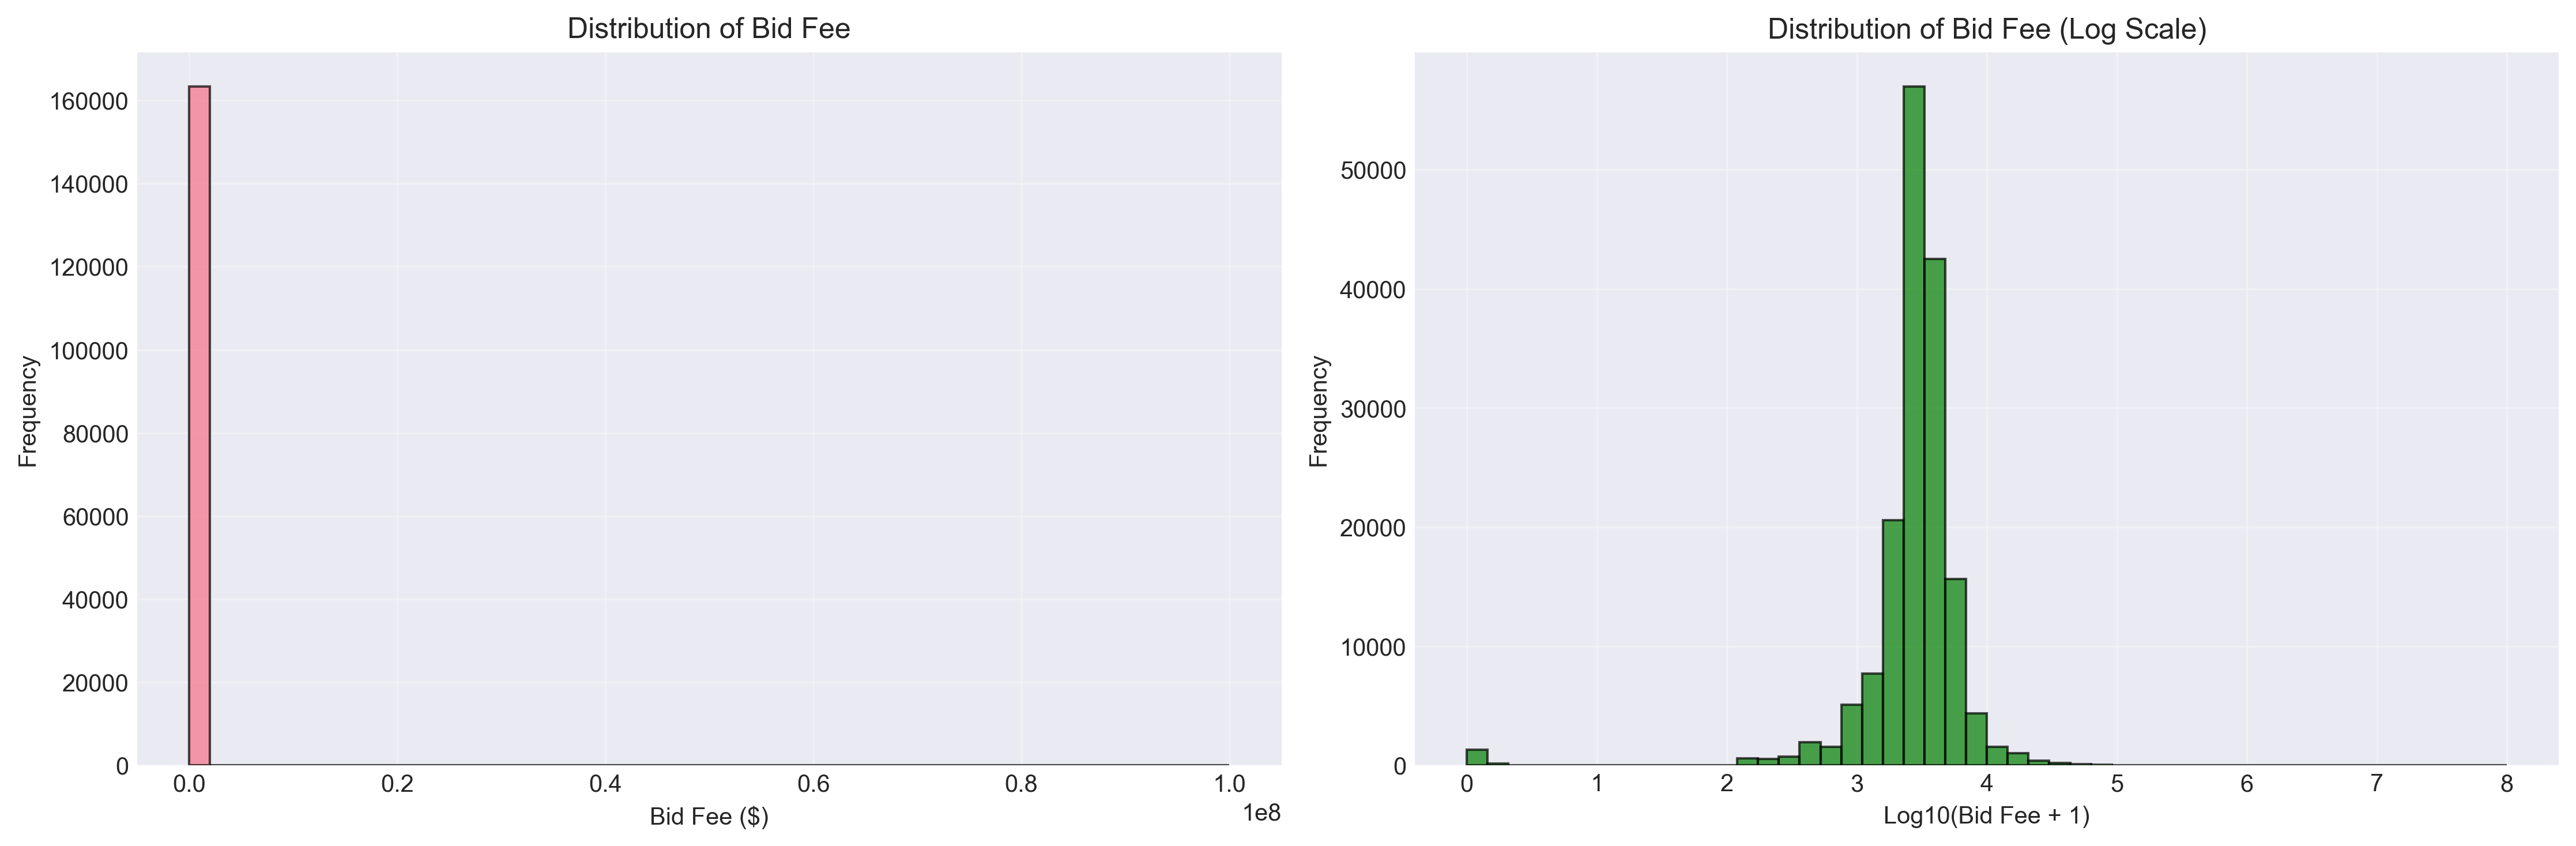
\includegraphics[width=0.85\textwidth]{bidfee_distribution.png}
\caption{Distribution of BidFee values after preprocessing, showing the right-skewed nature of engagement pricing.}
\label{fig:bidfee-dist}
\end{figure}

\subsection{Business Segment Distribution}

The dataset is dominated by the \textbf{Financing} segment, which accounts for the vast majority of bid records. Understanding this distribution is critical because the model's accuracy varies by segment data availability.

\begin{table}[H]
\centering
\caption{Business Segment Distribution}
\label{tab:segment-dist}
\begin{tabular}{lrr}
\toprule
\textbf{Business Segment} & \textbf{Record Count} & \textbf{Percentage} \\
\midrule
Financing & 92,945 & 81.2\% \\
Unknown & 12,116 & 10.6\% \\
Litigation & 3,128 & 2.7\% \\
Due Diligence & 2,481 & 2.2\% \\
Tax & 1,574 & 1.4\% \\
Insurance & 1,163 & 1.0\% \\
Other segments & $<$1\% each & 0.9\% \\
\bottomrule
\end{tabular}
\end{table}

Segments with more data naturally produce more confident predictions. The confidence scoring system (Section~\ref{sec:confidence}) explicitly accounts for segment sample size.

\subsection{Geographic Distribution}

\begin{figure}[H]
\centering
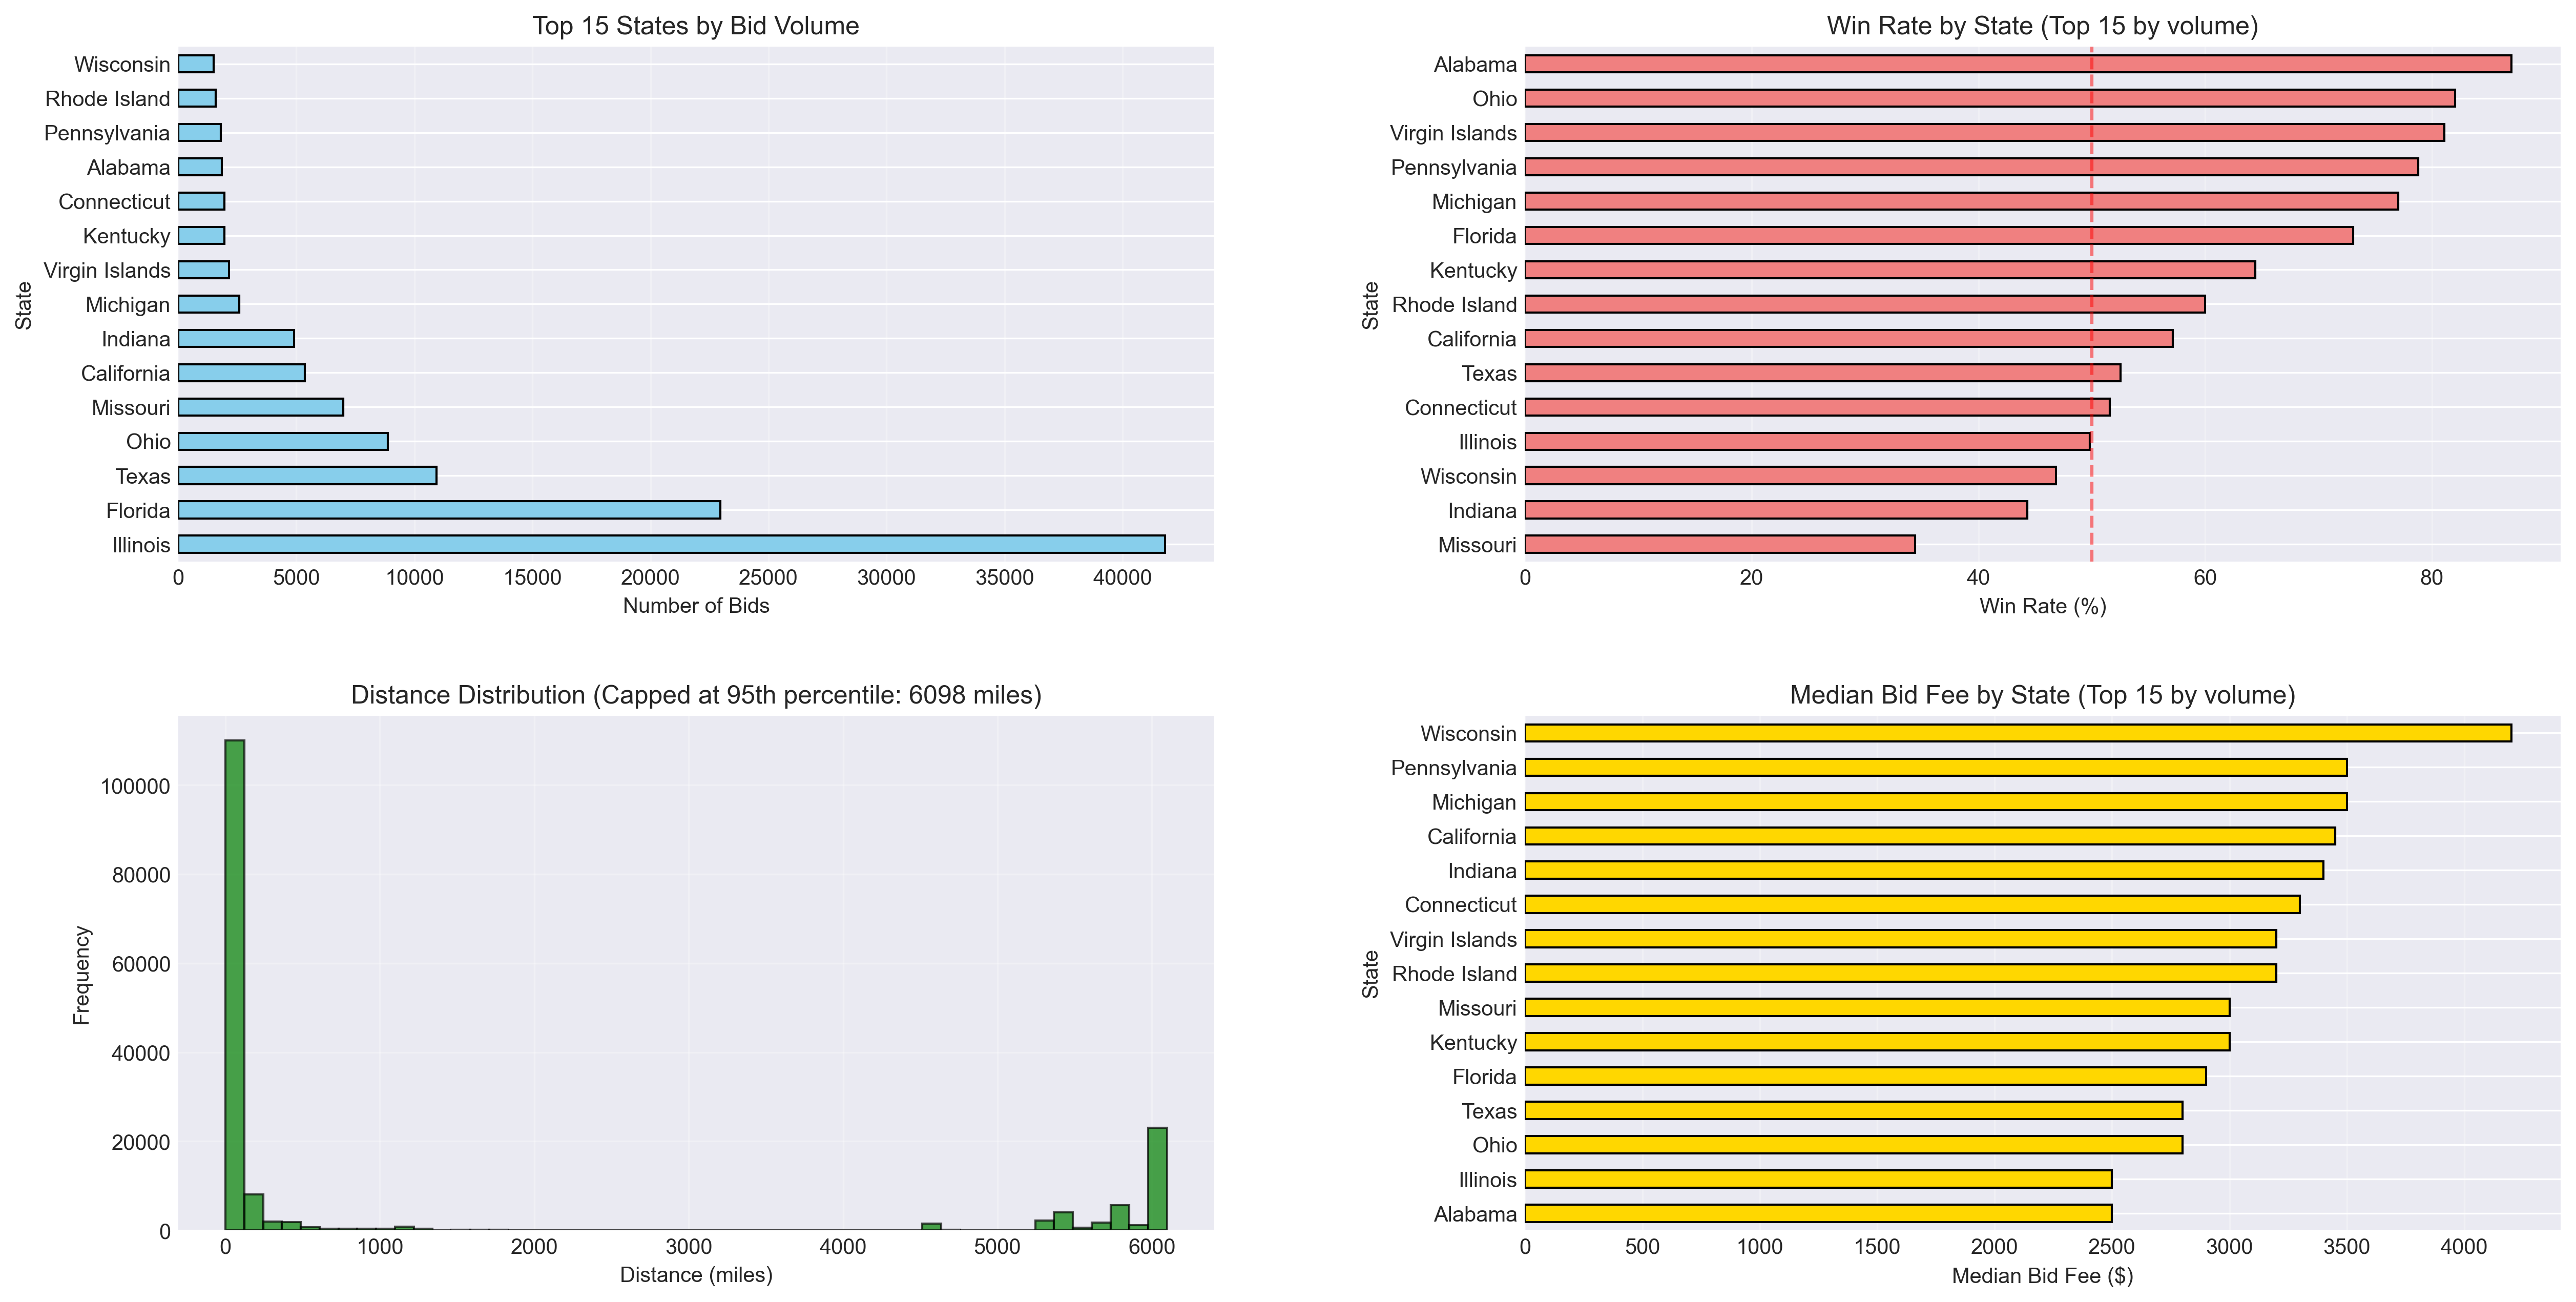
\includegraphics[width=0.85\textwidth]{geographic_analysis.png}
\caption{Geographic distribution of bid records across U.S. states. Illinois, Florida, and Texas are the top three states by volume.}
\label{fig:geo-dist}
\end{figure}

The geographic concentration in Illinois (25\%), Florida (14\%), and Texas (7\%) affects model confidence: states with thousands of historical bids produce far more reliable predictions than states with fewer than 50 records.

\subsection{Temporal Patterns}

\begin{figure}[H]
\centering
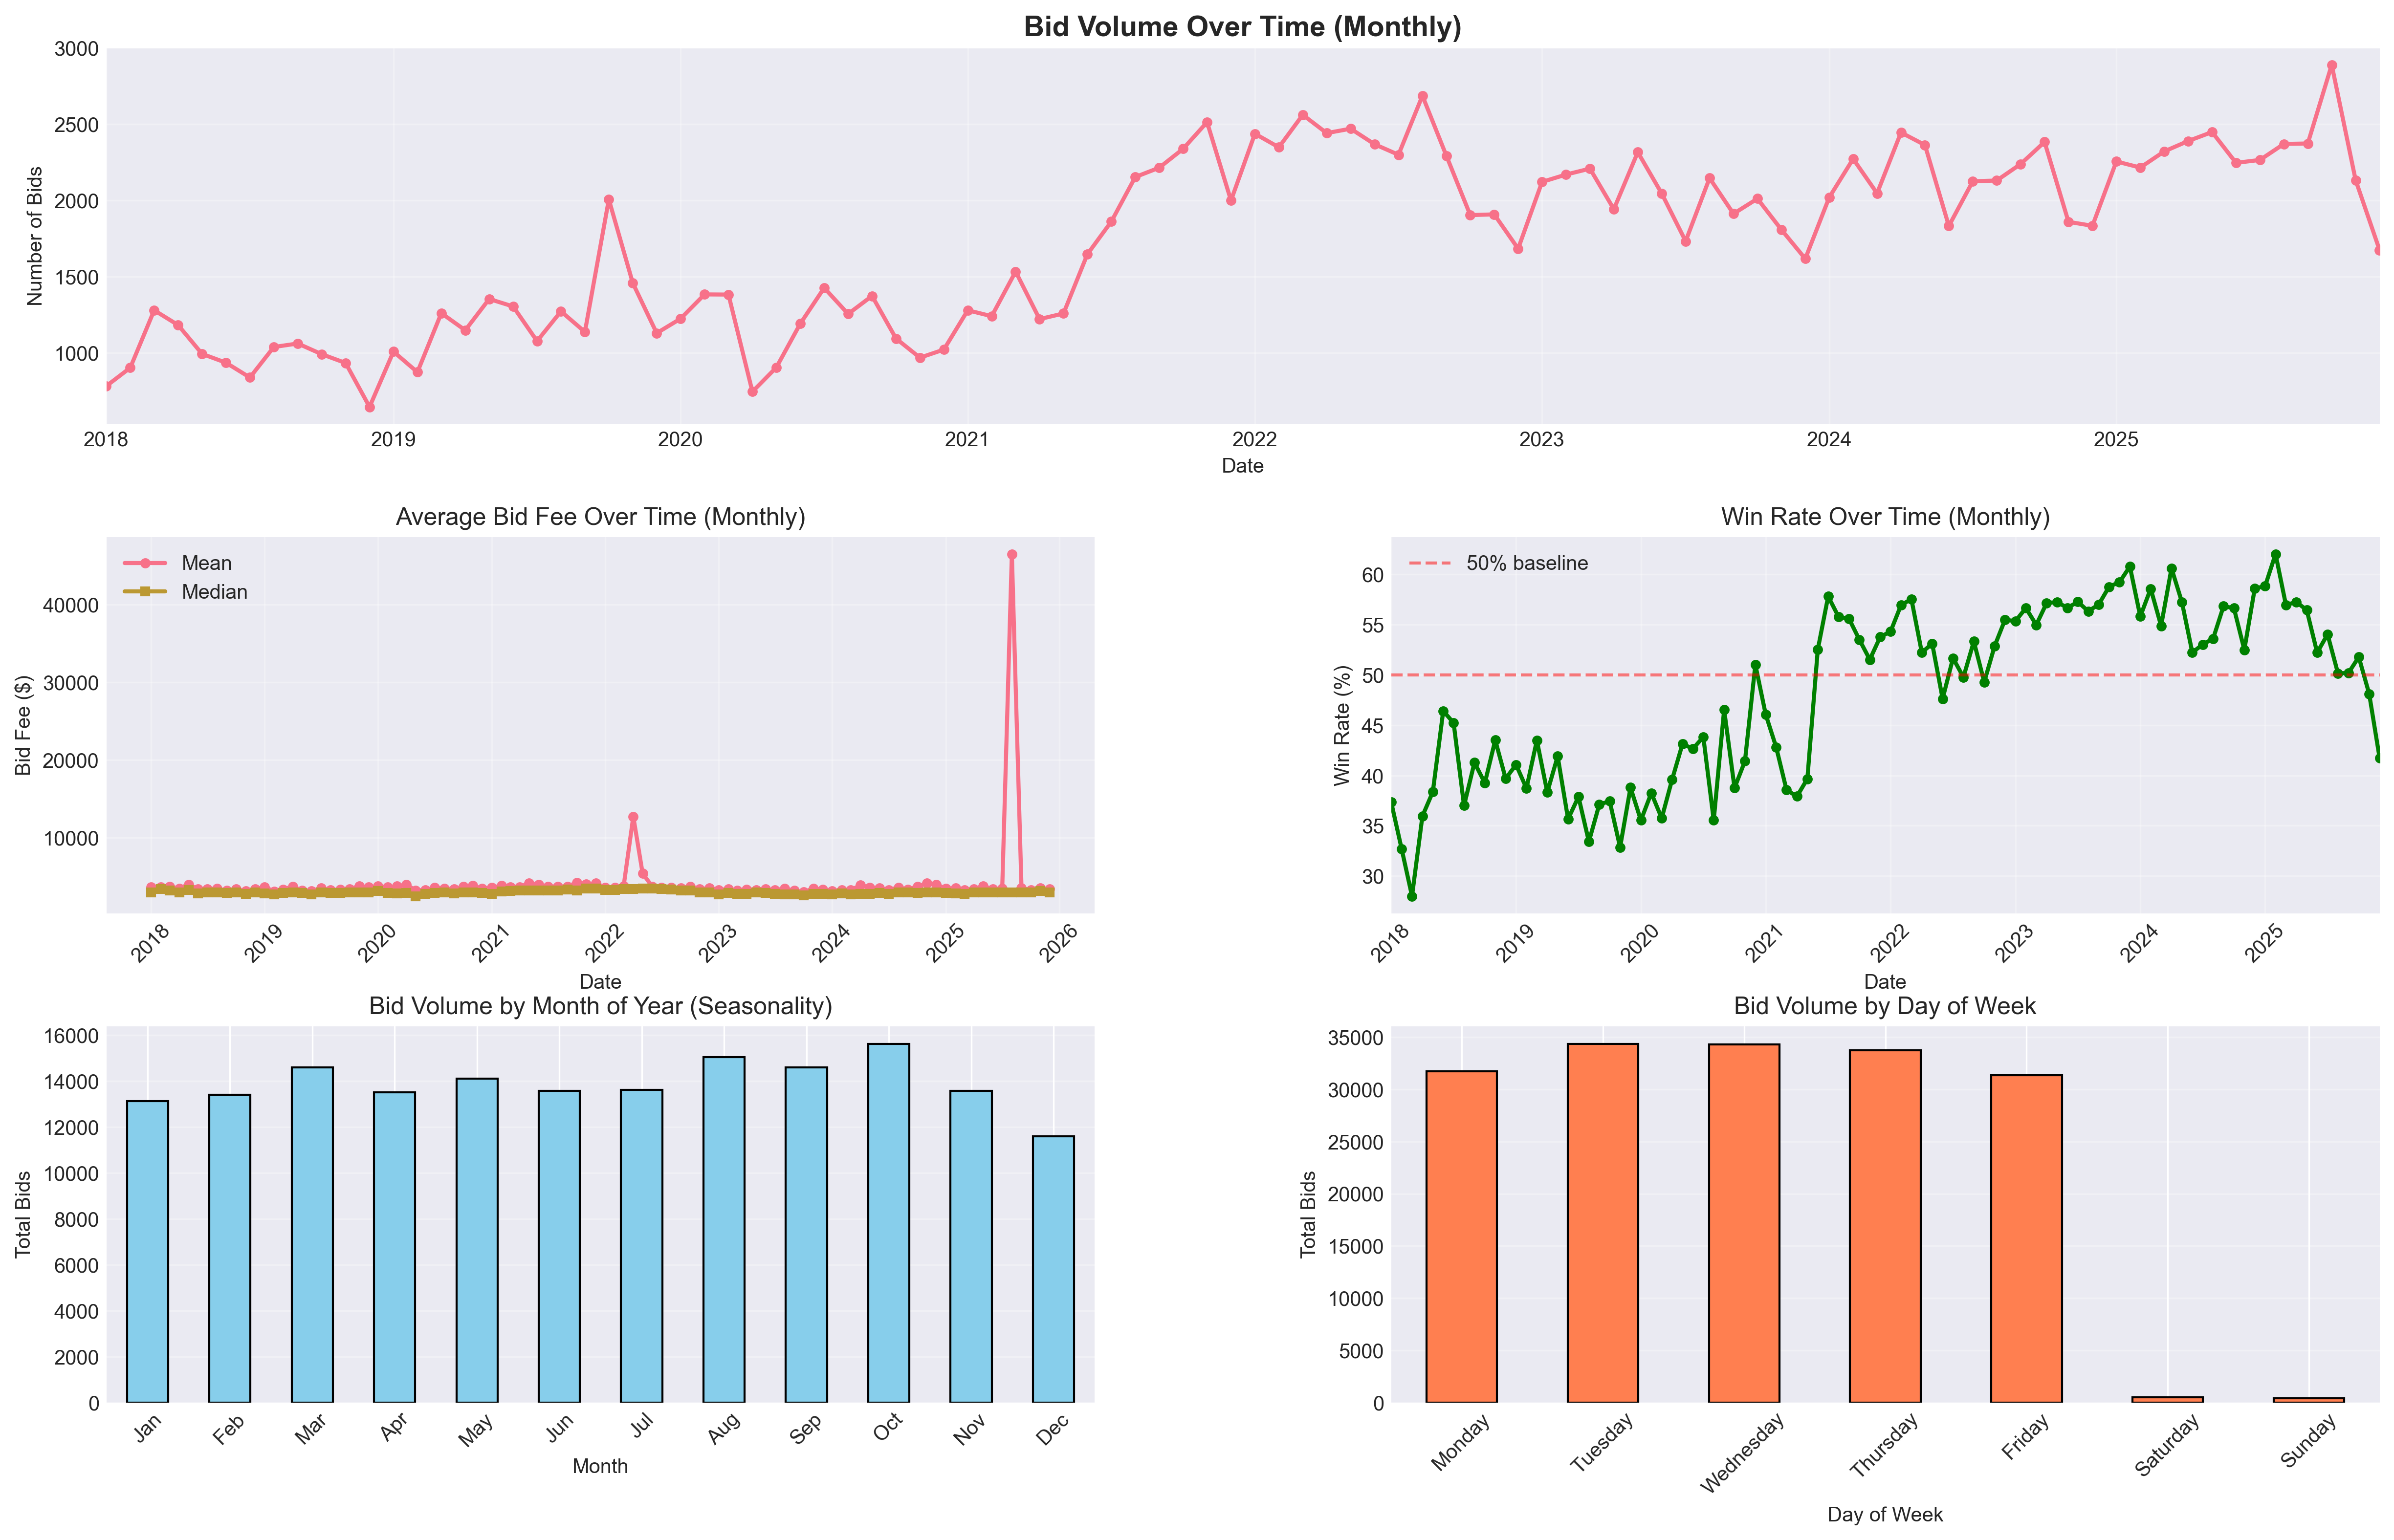
\includegraphics[width=0.85\textwidth]{time_series_analysis.png}
\caption{Time series analysis of bid volumes and fee trends, showing seasonal patterns and the 2023 regime shift.}
\label{fig:time-series}
\end{figure}

%============================================================================
\section{System Architecture}
%============================================================================

\subsection{High-Level Architecture}

The Bid Recommendation System is a full-stack application with three layers: a React frontend, a Flask REST API, and an offline ML training pipeline.

\begin{figure}[H]
\centering
\resizebox{\textwidth}{!}{%
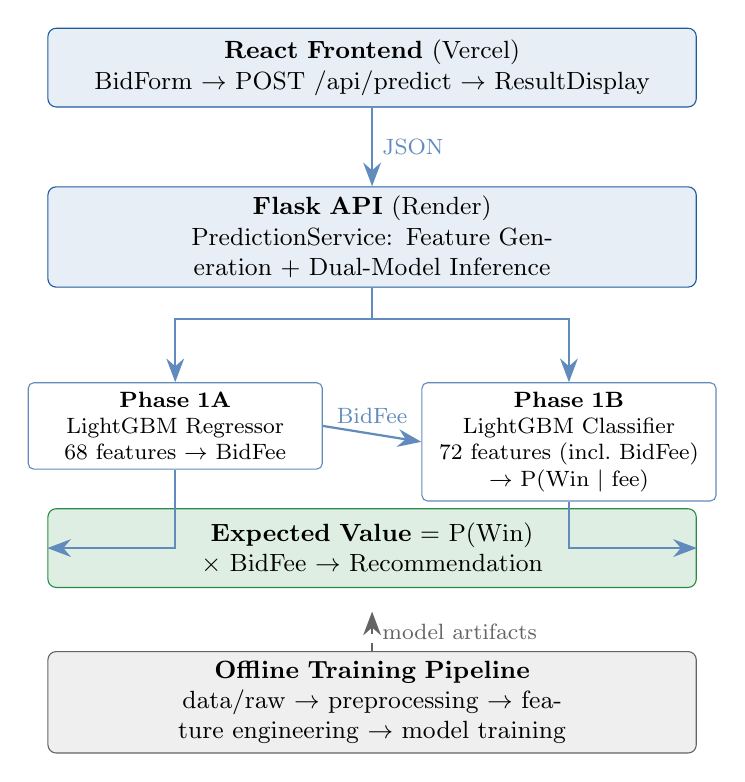
\begin{tikzpicture}[
    node distance=1.2cm,
    block/.style={rectangle, draw=gssblue, fill=gssblue!10, text width=8cm, minimum height=1cm, align=center, rounded corners=3pt, font=\small},
    smallblock/.style={rectangle, draw=gssblue!70, fill=white, text width=3.5cm, minimum height=0.9cm, align=center, rounded corners=2pt, font=\footnotesize},
    arrow/.style={-{Stealth[length=3mm]}, thick, gssblue!70}
]

% Frontend
\node[block] (frontend) {\textbf{React Frontend} (Vercel)\\BidForm $\to$ POST /api/predict $\to$ ResultDisplay};

% API
\node[block, below=1cm of frontend] (api) {\textbf{Flask API} (Render)\\PredictionService: Feature Generation + Dual-Model Inference};

% Models side by side — positioned manually to stay within bounds
\node[smallblock, below=1.2cm of api, xshift=-2.5cm] (regressor) {\textbf{Phase 1A}\\LightGBM Regressor\\68 features $\to$ BidFee};

\node[smallblock, below=1.2cm of api, xshift=2.5cm] (classifier) {\textbf{Phase 1B}\\LightGBM Classifier\\72 features (incl.\ BidFee)\\$\to$ P(Win $\mid$ fee)};

% EV node
\node[block, below=2.8cm of api, fill=gssgreen!15, draw=gssgreen] (ev) {\textbf{Expected Value} = P(Win) $\times$ BidFee $\to$ Recommendation};

% Training pipeline
\node[block, below=0.8cm of ev, fill=gssgray!10, draw=gssgray] (pipeline) {\textbf{Offline Training Pipeline}\\data/raw $\to$ preprocessing $\to$ feature engineering $\to$ model training};

% Arrows
\draw[arrow] (frontend) -- node[right, font=\footnotesize] {JSON} (api);
\draw[arrow] (api.south) -- ++(0,-0.4) -| (regressor.north);
\draw[arrow] (regressor.east) -- node[above, font=\footnotesize] {BidFee} (classifier.west);
\draw[arrow] (api.south) -- ++(0,-0.4) -| (classifier.north);
\draw[arrow] (regressor.south) |- (ev.west);
\draw[arrow] (classifier.south) |- (ev.east);
\draw[arrow, gssgray, dashed] (pipeline.north) -- ++(0, 0.5) node[right, font=\footnotesize, pos=0.5] {model artifacts};

\end{tikzpicture}%
}
\caption{System architecture: end-to-end flow from user input to bid recommendation.}
\label{fig:architecture}
\end{figure}

\subsection{Component Details}

\begin{description}[style=nextline]
    \item[\textbf{React Frontend (Vercel)}]
    Interactive web interface with a bid input form (6 fields: Business Segment, Property Type, State, Office, Target Time, Distance) and a results display showing predicted fee, confidence interval, win probability, expected value, and actionable recommendation.

    \item[\textbf{Flask API (Render)}]
    RESTful API that receives bid parameters, generates engineered features from 6 raw inputs using precomputed statistics, runs dual-model inference (injecting the predicted fee into the win probability model), and returns a structured JSON response.

    \item[\textbf{ML Training Pipeline (Offline)}]
    Sequential scripts that process raw bid data through cleaning, feature engineering (68 features across 9 categories), and model training. Outputs portable LightGBM \texttt{.txt} model files and metadata JSON for deployment.

    \item[\textbf{Configuration Layer}]
    Centralized \texttt{model\_config.py} with all hyperparameters, paths, feature exclusions, data filtering dates, and prediction service parameters. No hardcoded values in production code.
\end{description}

\subsection{Prediction Flow}

When a user submits a bid request, the following steps occur:

\begin{enumerate}[nosep]
    \item \textbf{Feature Generation:} 6 raw inputs are transformed into 68 features using precomputed group statistics (segment averages, state benchmarks, rolling means, etc.).
    \item \textbf{Phase 1A --- Bid Fee Prediction:} The LightGBM regression model predicts the optimal fee, with empirical confidence bands.
    \item \textbf{Phase 1B --- Win Probability:} The predicted fee is injected as the \texttt{BidFee} feature into the LightGBM classifier, which predicts $P(\text{Win} \mid \text{context}, \text{fee})$ directly. The fee is compared against a blended benchmark (segment + state + property type weighted average) for recommendation context.
    \item \textbf{Expected Value Calculation:} $\text{EV} = P(\text{Win}) \times \text{BidFee}$.
    \item \textbf{Recommendation Generation:} Contextual recommendation based on fee relative to blended market benchmark and win probability level.
\end{enumerate}

\subsection{Deployment Configuration}

\begin{table}[H]
\centering
\caption{Deployment Configuration}
\label{tab:deployment}
\begin{tabular}{lll}
\toprule
\textbf{Component} & \textbf{Platform} & \textbf{Details} \\
\midrule
Frontend & Vercel & Auto-deploys from \texttt{/frontend} \\
API & Render & \texttt{gunicorn api.app:app}, 120s timeout \\
Python version & 3.11.0 & Specified in \texttt{.python-version} \\
Model format & LightGBM \texttt{.txt} & Portable, version-controllable \\
\bottomrule
\end{tabular}
\end{table}

%============================================================================
\section{Feature Engineering}
\label{sec:feature-engineering}
%============================================================================

Feature engineering is the most critical component of the system. Raw numerical features (TargetTime, Distance, demographics) have near-zero correlation with BidFee individually ($r < 0.012$). The predictive power comes almost entirely from \textbf{engineered aggregate and contextual features}.

\subsection{Feature Categories Overview}

A total of 68 features are used by the production bid fee model, organized into 9 categories:

\begin{table}[H]
\centering
\caption{Feature Engineering Categories}
\label{tab:feature-categories}
\begin{tabular}{clcl}
\toprule
\textbf{\#} & \textbf{Category} & \textbf{Count} & \textbf{Description} \\
\midrule
1 & Rolling/Time Series & 7 & 90-day rolling means, counts, std devs \\
2 & Client Lag Features & 4 & Previous fee, days since last bid, etc. \\
3 & Cumulative Client & 4 & Total bids/wins, win rate, avg fee \\
4 & Aggregation Features & 15 & Office/state/segment/property/client avgs \\
5 & Interaction Features & 4 & Cross-feature products \\
6 & Categorical Encodings & 14 & Frequency and label encodings \\
7 & Temporal Trends & 4 & Days since start, quarterly avg, season \\
8 & Ratio Features & 4 & Fee/time ratios to group averages \\
9 & Utility Features & 2 & Building size numeric, fee z-score \\
\midrule
& \textbf{Total (before selection)} & \textbf{84} & \\
& \textbf{Total (after SHAP selection)} & \textbf{68} & \\
\bottomrule
\end{tabular}
\end{table}

\subsection{Leakage Prevention: Leave-One-Out Aggregation}

A critical design decision is the use of \textbf{leave-one-out (LOO) aggregation} for all target-derived features. When computing \texttt{segment\_avg\_fee} for row $i$, row $i$'s own BidFee is excluded:

\begin{equation}
\texttt{segment\_avg\_fee}_i = \frac{\sum_{j \in \text{segment}, j \neq i} \text{BidFee}_j}{|\text{segment}| - 1}
\end{equation}

Without LOO, each row would partially contain its own target value in its features, creating target leakage that inflates metrics but fails in production.

\subsection{Key Feature Insights}

\begin{figure}[H]
\centering
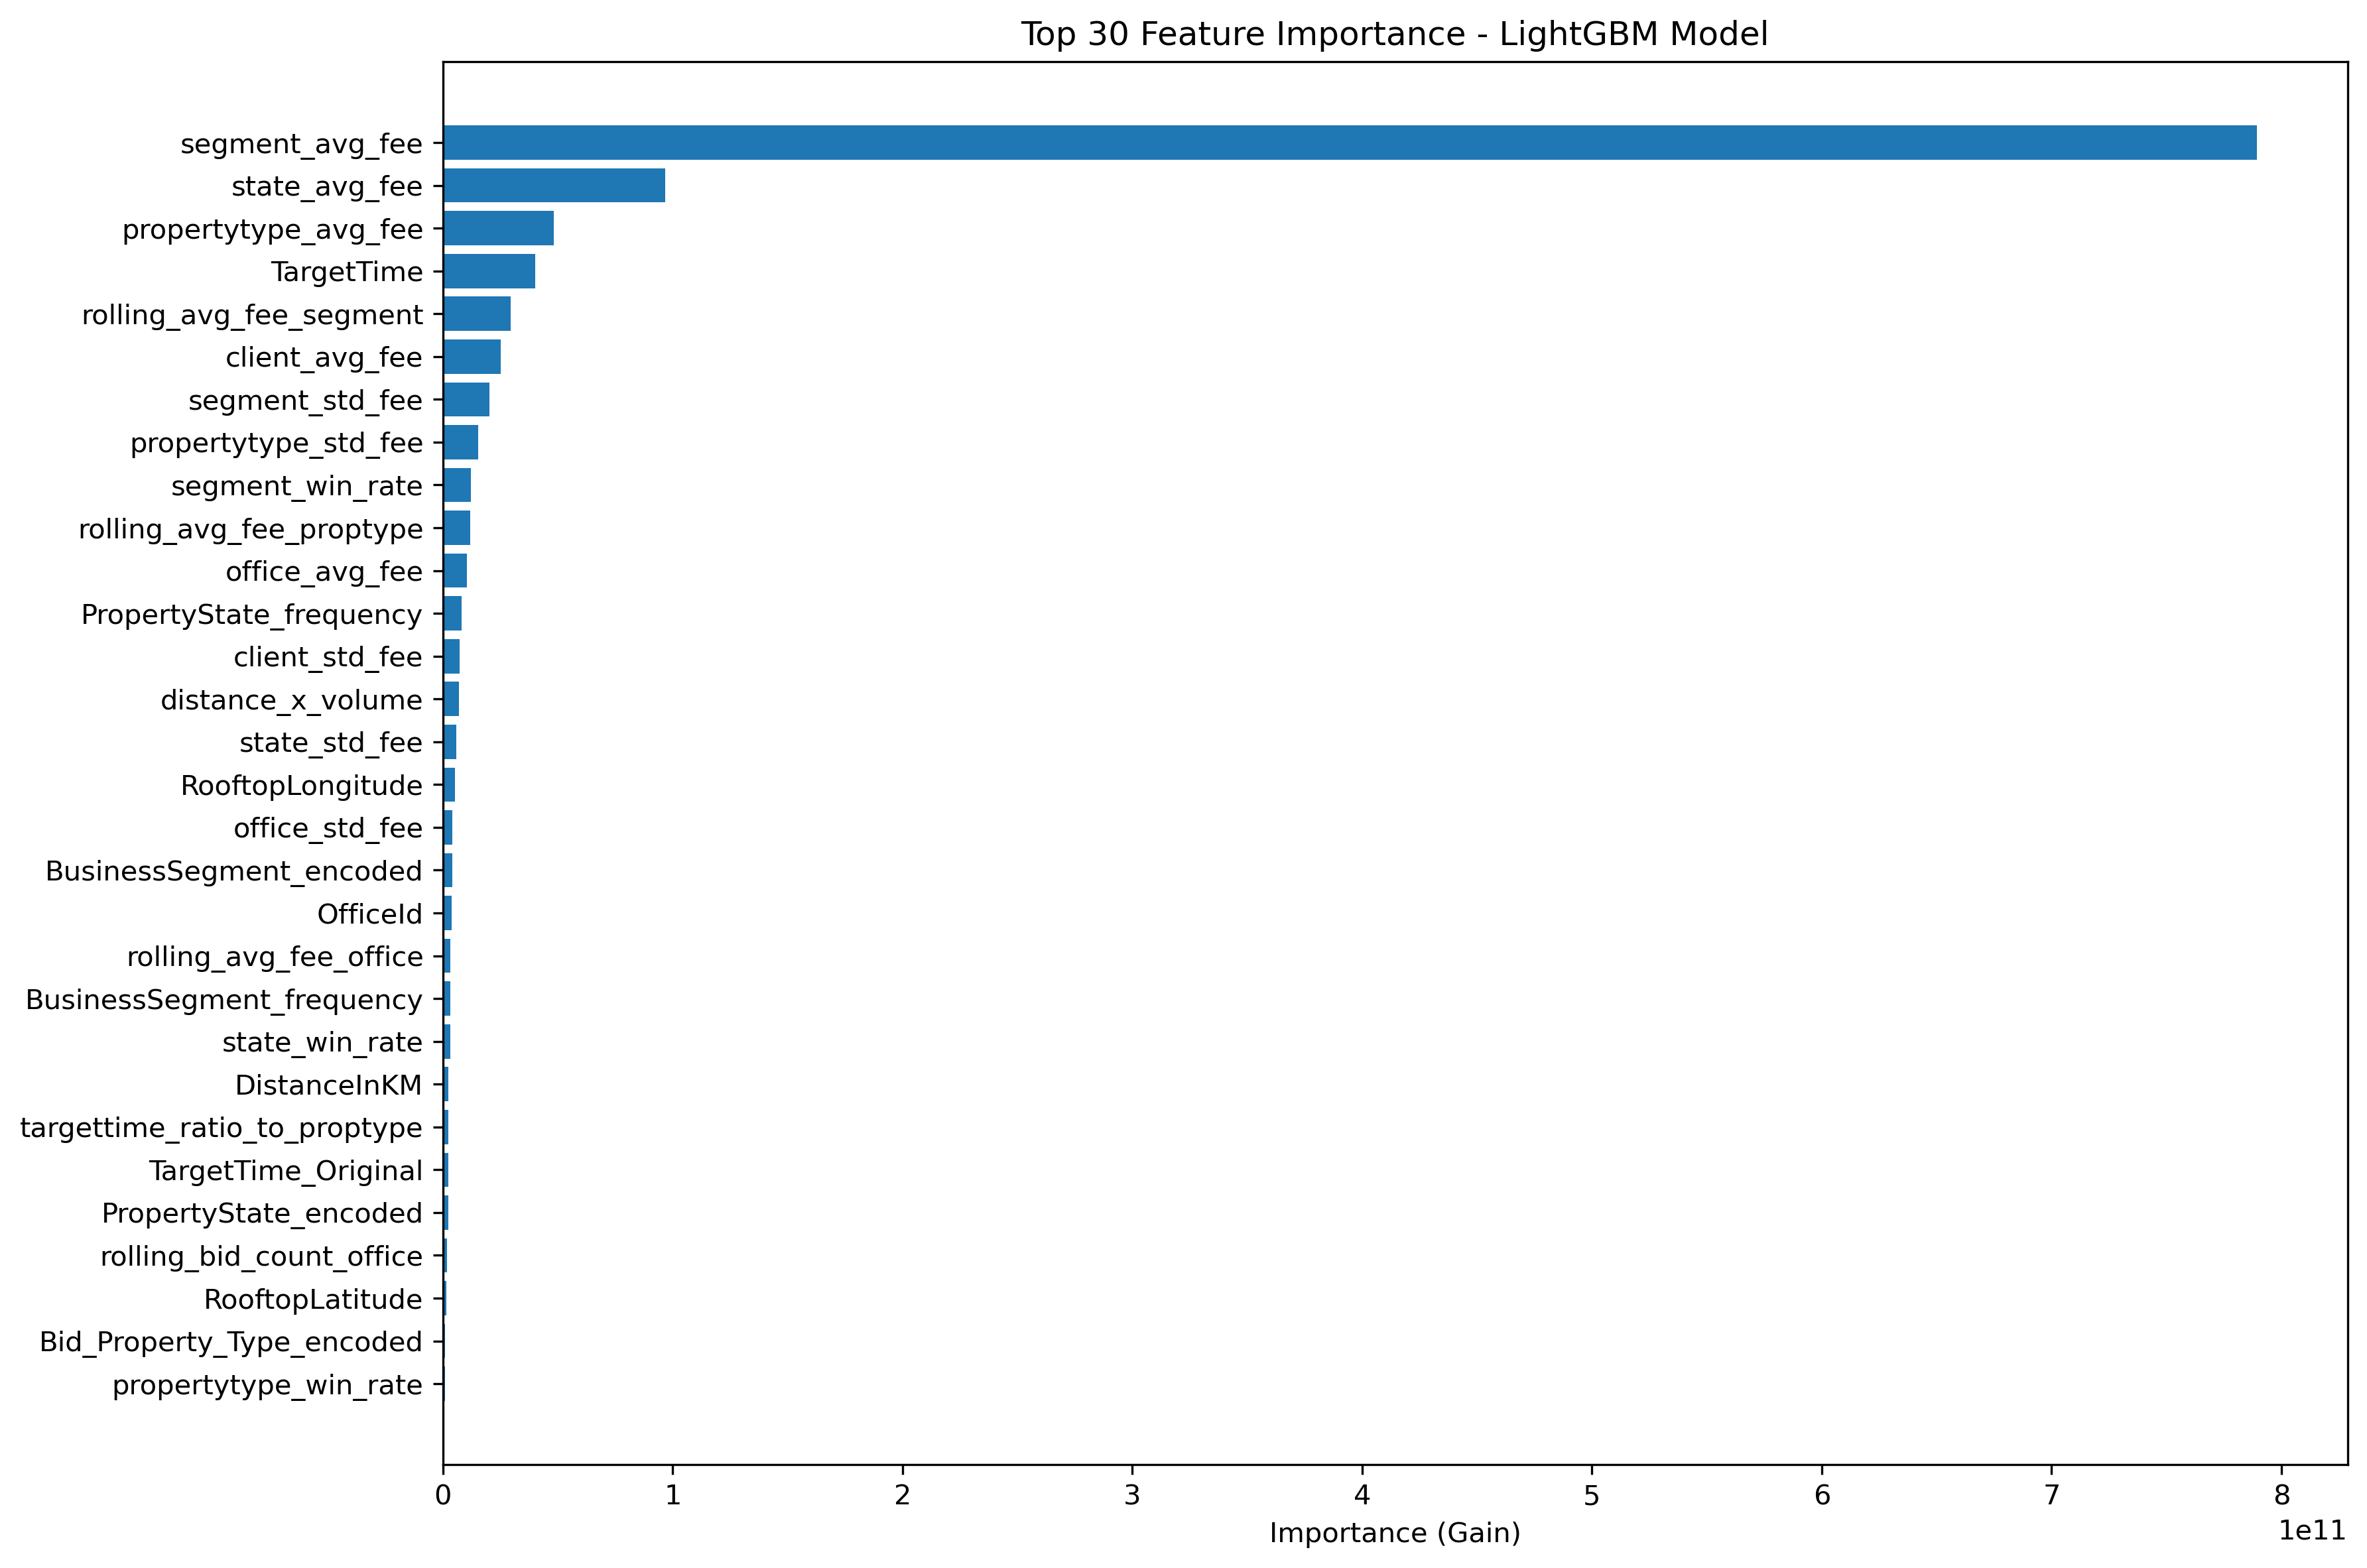
\includegraphics[width=0.95\textwidth]{lightgbm_feature_importance.png}
\caption{Top 30 features by LightGBM split-gain importance for the bid fee model. \texttt{segment\_avg\_fee} alone accounts for the dominant share of predictive power.}
\label{fig:feature-importance}
\end{figure}

The \textbf{segment average fee} (\texttt{segment\_avg\_fee}) is overwhelmingly the most important feature, contributing approximately 64\% of the model's total split-gain importance. This aligns with the business intuition: bid pricing is primarily driven by market context (what segment you are in and what similar engagements typically cost), not by individual deal characteristics.

\begin{table}[H]
\centering
\caption{Top 10 Features --- Bid Fee Model (LightGBM)}
\label{tab:top-features-bidfee}
\begin{tabular}{clr}
\toprule
\textbf{Rank} & \textbf{Feature} & \textbf{Importance (\%)} \\
\midrule
1 & \texttt{segment\_avg\_fee} & 64.0\% \\
2 & \texttt{state\_avg\_fee} & 7.8\% \\
3 & \texttt{propertytype\_avg\_fee} & 3.9\% \\
4 & \texttt{TargetTime} & 3.3\% \\
5 & \texttt{rolling\_avg\_fee\_segment} & 2.4\% \\
6 & \texttt{client\_avg\_fee} & 2.1\% \\
7 & \texttt{segment\_std\_fee} & 1.7\% \\
8 & \texttt{propertytype\_std\_fee} & 1.3\% \\
9 & \texttt{segment\_win\_rate} & 1.0\% \\
10 & \texttt{rolling\_avg\_fee\_proptype} & 1.0\% \\
\bottomrule
\end{tabular}
\end{table}

\subsection{Feature Selection: SHAP-Based Backward Elimination}
\label{sec:feature-selection}

Starting from the full 84-feature set, we performed systematic backward elimination guided by SHAP values. Features were removed in 10\% increments, and model performance was evaluated at each step.

\begin{table}[H]
\centering
\caption{Feature Ablation Results: Impact of Feature Reduction on Test RMSE}
\label{tab:feature-ablation}
\begin{tabular}{cccc}
\toprule
\textbf{Removal \%} & \textbf{Features} & \textbf{Test RMSE (\$)} & \textbf{RMSE Change (\%)} \\
\midrule
0\% (baseline) & 84 & 349.32 & --- \\
10\% & 76 & 339.73 & $-$2.75\% \\
\textbf{20\%} & \textbf{68} & \textbf{328.75} & $\mathbf{-5.89\%}$ \\
30\% & 59 & 338.78 & $-$3.02\% \\
40\% & 51 & 332.80 & $-$4.73\% \\
50\% & 42 & 352.01 & $+$0.77\% \\
\bottomrule
\end{tabular}
\end{table}

The optimal configuration uses \textbf{68 features} (20\% reduction), which achieves a \textbf{5.89\% improvement} in test RMSE over the full feature set. Removing more features degrades performance, confirming that the 68-feature set captures the essential signal.

\begin{figure}[H]
\centering
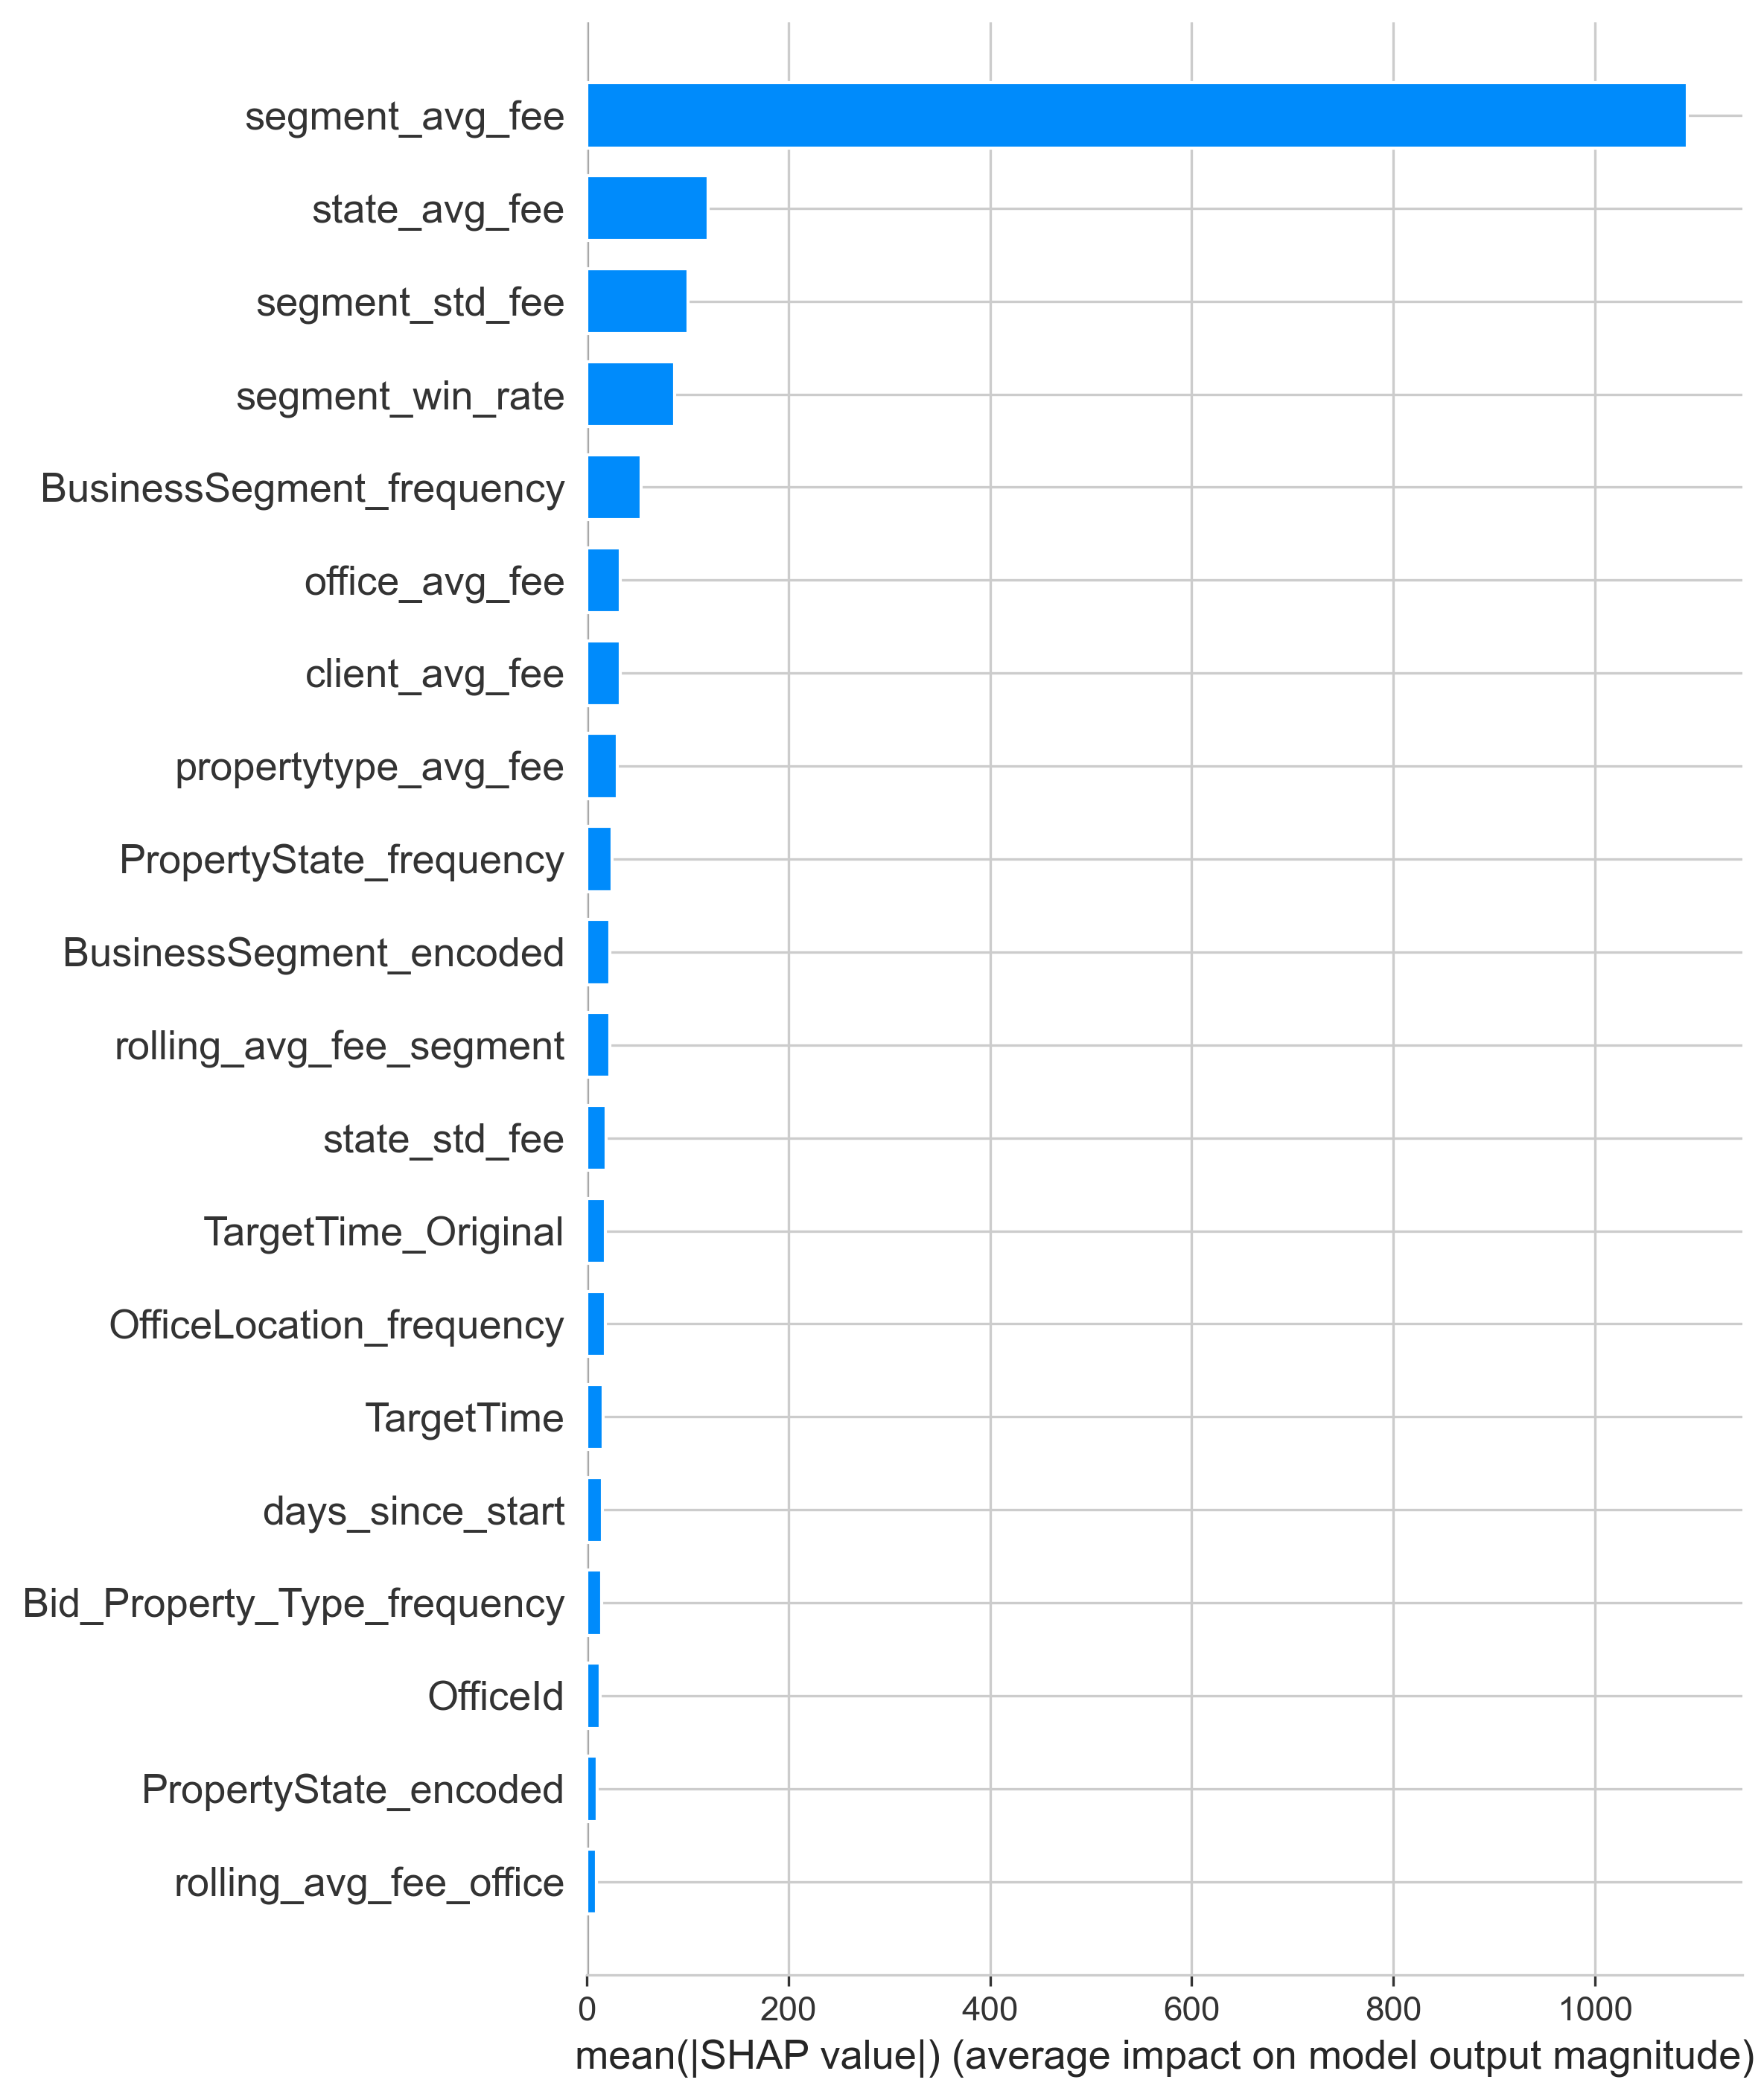
\includegraphics[width=0.85\textwidth]{shap_feature_importance.png}
\caption{SHAP summary plot showing the direction and magnitude of feature impacts on bid fee predictions.}
\label{fig:shap-summary}
\end{figure}

%============================================================================
\section{Model Development}
%============================================================================

\subsection{Model Selection Rationale}

We evaluated multiple model families before selecting LightGBM:

\begin{itemize}[nosep]
    \item \textbf{Econometric panel models} (Pooled OLS, Fixed Effects, Random Effects) --- standard approaches in real estate economics but unable to capture non-linear feature interactions.
    \item \textbf{XGBoost} --- strong gradient boosting baseline, but underperforms LightGBM on this dataset.
    \item \textbf{LightGBM} --- selected for superior accuracy, faster training, native categorical support, and excellent handling of high-cardinality features.
\end{itemize}

\subsection{Phase 1A: Bid Fee Prediction (Regression)}

\subsubsection{Model Configuration}

\begin{table}[H]
\centering
\caption{LightGBM Regression Hyperparameters}
\label{tab:lgb-regression-params}
\begin{tabular}{ll}
\toprule
\textbf{Parameter} & \textbf{Value} \\
\midrule
Objective & Regression (L2 loss) \\
Boosting type & GBDT \\
Number of leaves & 18 \\
Maximum depth & 8 \\
Learning rate & 0.05 \\
Feature fraction & 0.8 \\
Bagging fraction & 0.8 \\
Bagging frequency & 5 \\
Min child samples & 30 \\
Min child weight & 5 \\
L1 regularization ($\alpha$) & 2.0 \\
L2 regularization ($\lambda$) & 2.0 \\
Number of boosting rounds & 500 \\
Early stopping rounds & 50 \\
\bottomrule
\end{tabular}
\end{table}

The regularization parameters ($\alpha = 2.0$, $\lambda = 2.0$) and reduced leaf count (18) were specifically tuned to control overfitting, bringing the train/test RMSE ratio down to 1.99$\times$ (target: $<2.0\times$).

\subsubsection{Results}

\begin{table}[H]
\centering
\caption{Phase 1A: Bid Fee Model Performance}
\label{tab:bidfee-results}
\begin{tabular}{lrrr}
\toprule
\textbf{Metric} & \textbf{Train} & \textbf{Validation} & \textbf{Test} \\
\midrule
RMSE (\$) & 177.63 & 361.10 & 353.99 \\
MAE (\$) & --- & --- & 108.63 \\
Median AE (\$) & --- & --- & 35.16 \\
$R^2$ & --- & --- & 0.9723 \\
MAPE (\%) & --- & --- & 71.18 \\
Overfitting ratio & \multicolumn{3}{c}{1.99$\times$} \\
Best iteration & \multicolumn{3}{c}{500} \\
\bottomrule
\end{tabular}
\end{table}

The model achieves a test $R^2$ of 0.9723, meaning it explains 97.2\% of the variance in bid fees. The median absolute error of \$35.16 indicates that half of all predictions are within \$35 of the actual bid fee. The elevated MAPE (71.18\%) is driven by very small-value bids where even small absolute errors produce large percentage errors.

\begin{figure}[H]
\centering
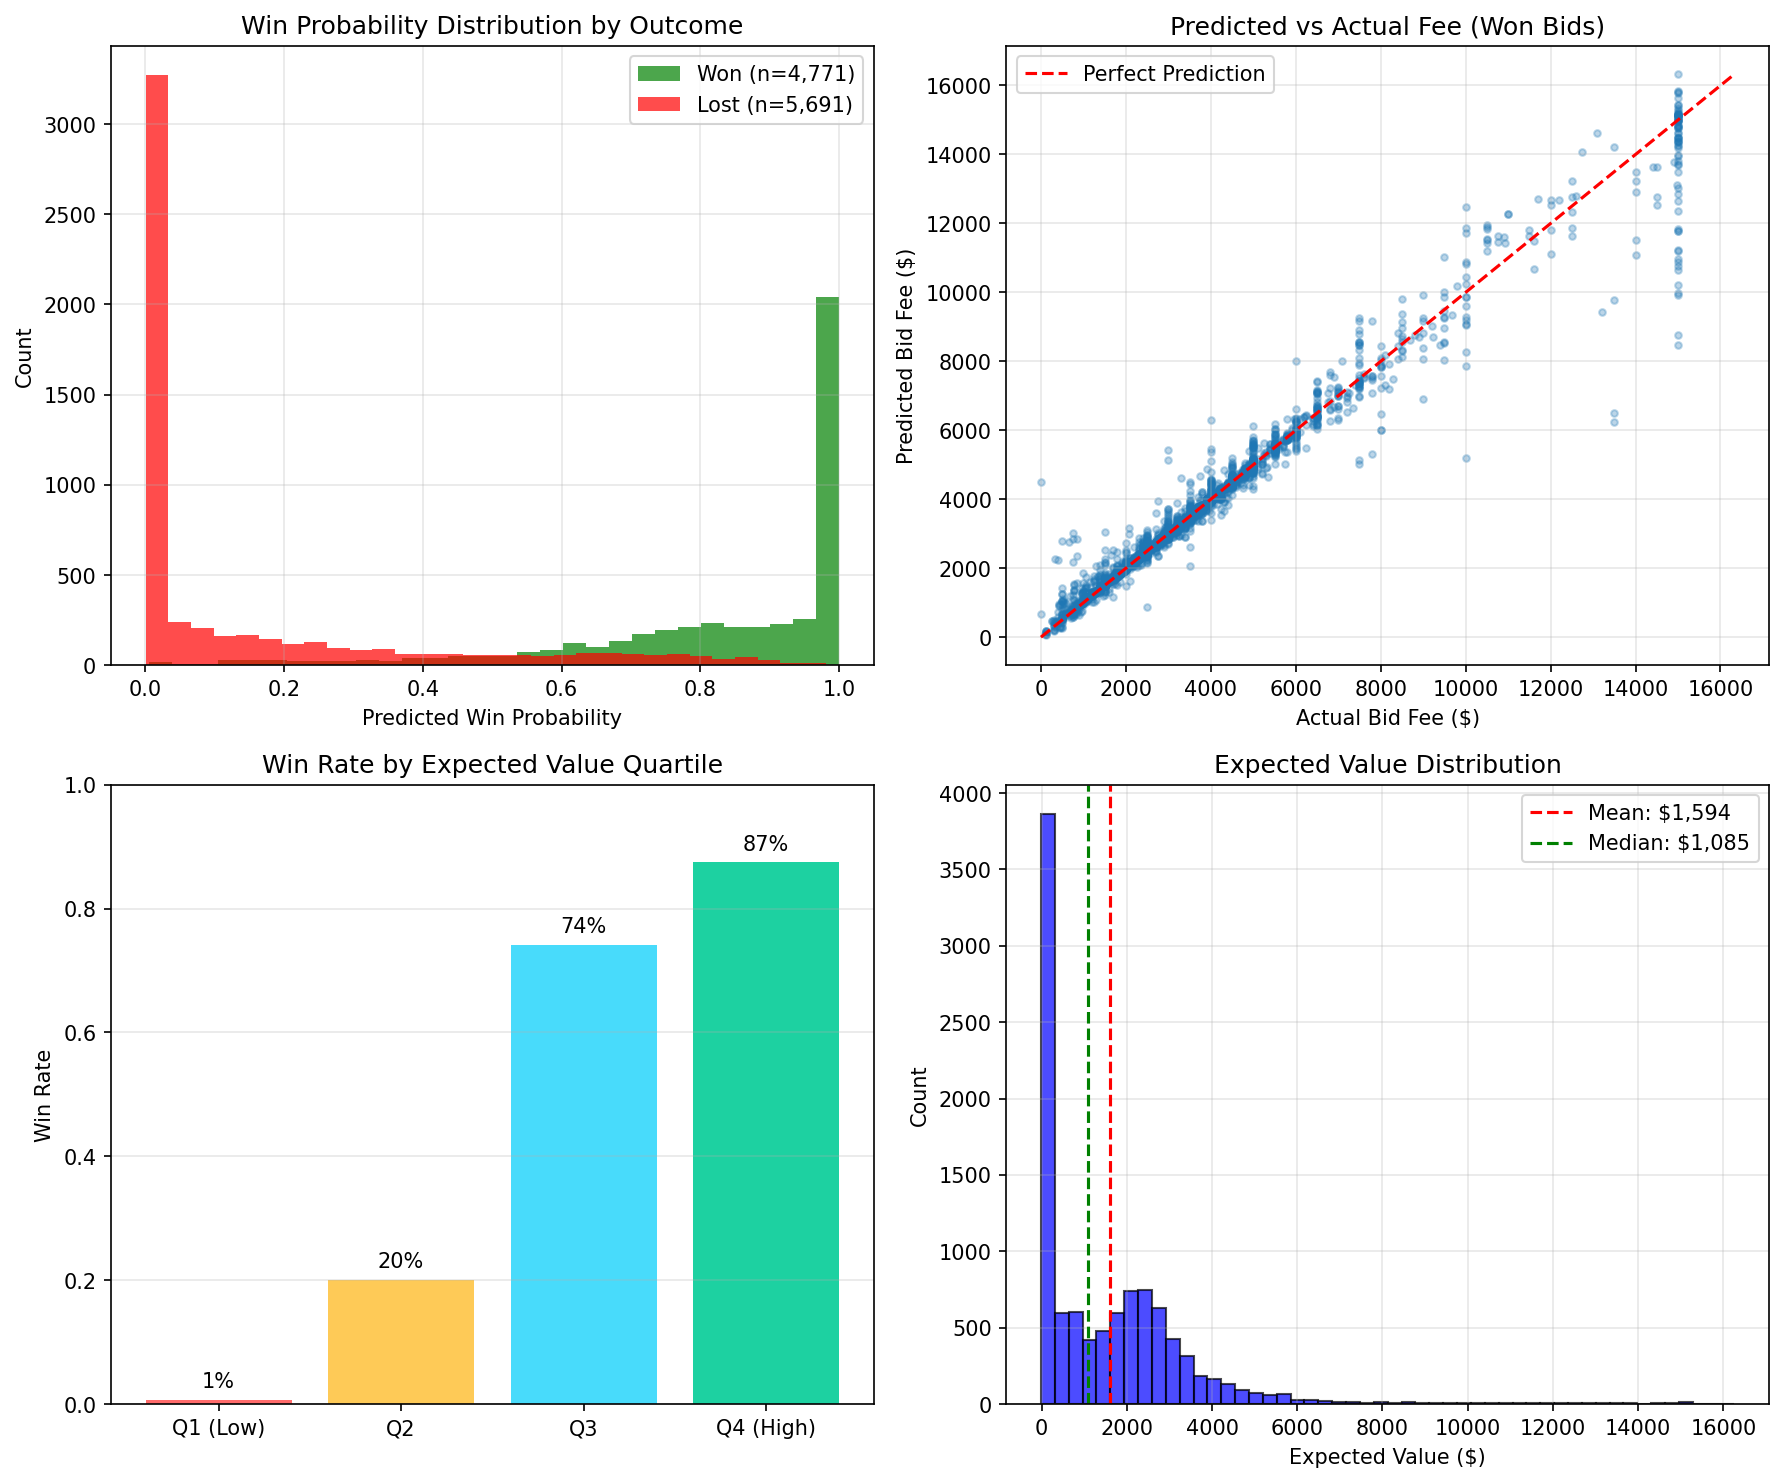
\includegraphics[width=0.85\textwidth]{model_validation.png}
\caption{Model validation: predicted vs.\ actual bid fees, residual distribution, and performance across segments.}
\label{fig:model-validation}
\end{figure}

\begin{figure}[H]
\centering
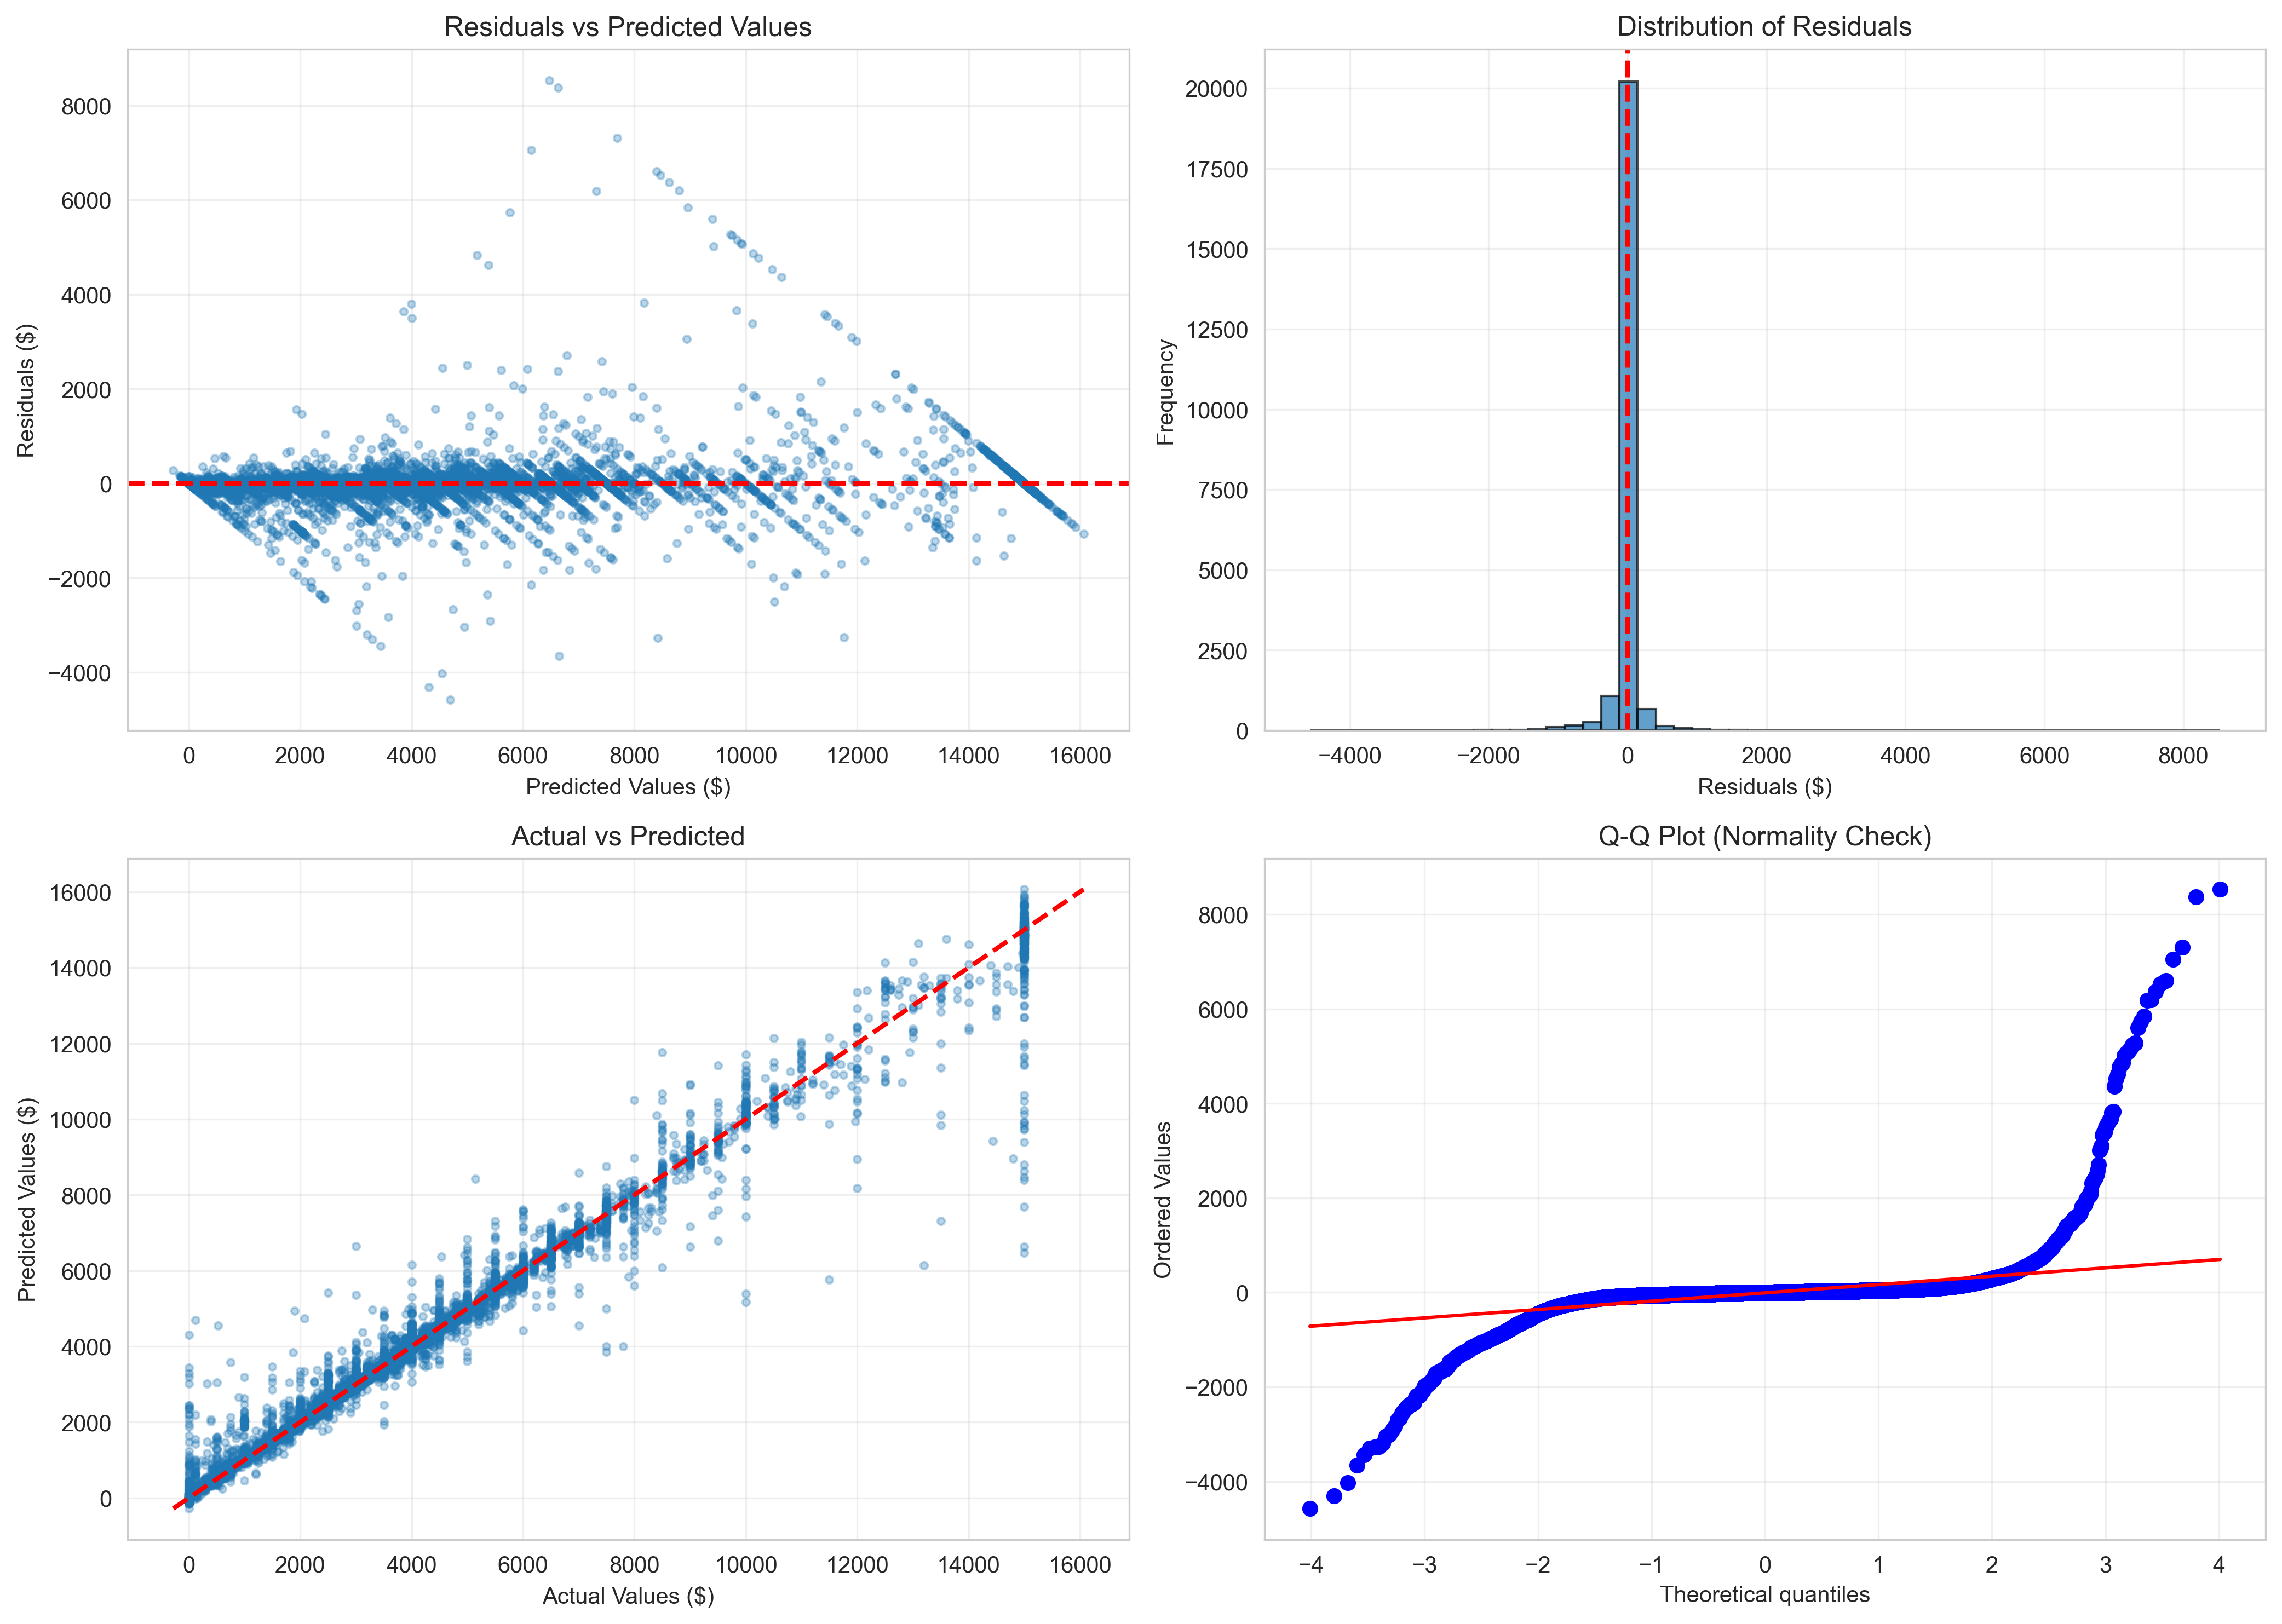
\includegraphics[width=0.85\textwidth]{model_residual_analysis.png}
\caption{Residual analysis showing homoscedastic error patterns and no systematic bias.}
\label{fig:residual-analysis}
\end{figure}

\subsection{Phase 1B: Win Probability Prediction (Classification)}

\subsubsection{Model Configuration}

\begin{table}[H]
\centering
\caption{LightGBM Classification Hyperparameters}
\label{tab:lgb-classification-params}
\begin{tabular}{ll}
\toprule
\textbf{Parameter} & \textbf{Value} \\
\midrule
Objective & Binary (log loss) \\
Boosting type & GBDT \\
Number of leaves & 20 \\
Maximum depth & 8 \\
Learning rate & 0.05 \\
Feature fraction & 0.8 \\
Bagging fraction & 0.8 \\
Min child samples & 30 \\
L1 regularization ($\alpha$) & 1.0 \\
L2 regularization ($\lambda$) & 1.0 \\
Scale positive weight & 1.052 \\
Best iteration & 415 (early stopped) \\
\bottomrule
\end{tabular}
\end{table}

The classification model uses 72 features. Critically, 9 \textbf{leaky features} are excluded (win rates, total wins) since they derive from the target variable \texttt{Won}. Additionally, 4 \textbf{job-derived features} (\texttt{JobCount}, \texttt{IECount}, \texttt{LeaseCount}, \texttt{SaleCount}) are excluded because they leak target information: these fields are \texttt{NULL} for lost bids (no job created) and populated for won bids. When filled with 0, the model learns ``JobCount=0 means lost'' --- a cheat code, not a real signal. The model \emph{includes} \texttt{BidFee} as a feature, allowing it to learn fee-sensitivity directly from historical outcomes (Section~\ref{sec:fee-adjustment}).

\subsubsection{Results}

\begin{table}[H]
\centering
\caption{Phase 1B: Win Probability Model Performance}
\label{tab:winprob-results}
\begin{tabular}{lrrr}
\toprule
\textbf{Metric} & \textbf{Train} & \textbf{Validation} & \textbf{Test} \\
\midrule
AUC-ROC & 0.945 & 0.906 & 0.870 \\
Accuracy & 86.4\% & 82.2\% & 79.0\% \\
Precision & 90.0\% & 87.0\% & 81.5\% \\
Recall & 81.2\% & 77.3\% & 69.8\% \\
F1 Score & 85.3\% & 81.8\% & 75.2\% \\
Brier Score & --- & --- & 0.140 \\
Train/Test AUC ratio & \multicolumn{3}{c}{1.09$\times$ (excellent generalization)} \\
\bottomrule
\end{tabular}
\end{table}

\begin{table}[H]
\centering
\caption{Confusion Matrix --- Win Probability Model (Test Set)}
\label{tab:confusion-matrix}
\begin{tabular}{lcc}
\toprule
& \textbf{Predicted Loss} & \textbf{Predicted Win} \\
\midrule
\textbf{Actual Loss} & 4,937 (TN) & 754 (FP) \\
\textbf{Actual Win} & 1,441 (FN) & 3,330 (TP) \\
\bottomrule
\end{tabular}
\end{table}

The train/test AUC ratio of 1.09$\times$ indicates excellent generalization --- the model performs nearly identically on unseen data. The Brier score of 0.140 reflects honest calibration; the model is well-calibrated at extreme probabilities (within $\pm$2\% for predictions below 20\% or above 90\%) but slightly overconfident in the 45--75\% range.

\textbf{Note on metrics:} An earlier version of this model reported AUC = 0.962 and accuracy = 89.2\%. These metrics were inflated by \texttt{JobCount} leakage (see Section~\ref{sec:data-integrity}). The current metrics reflect genuine predictive power from legitimate features.

\begin{figure}[H]
\centering
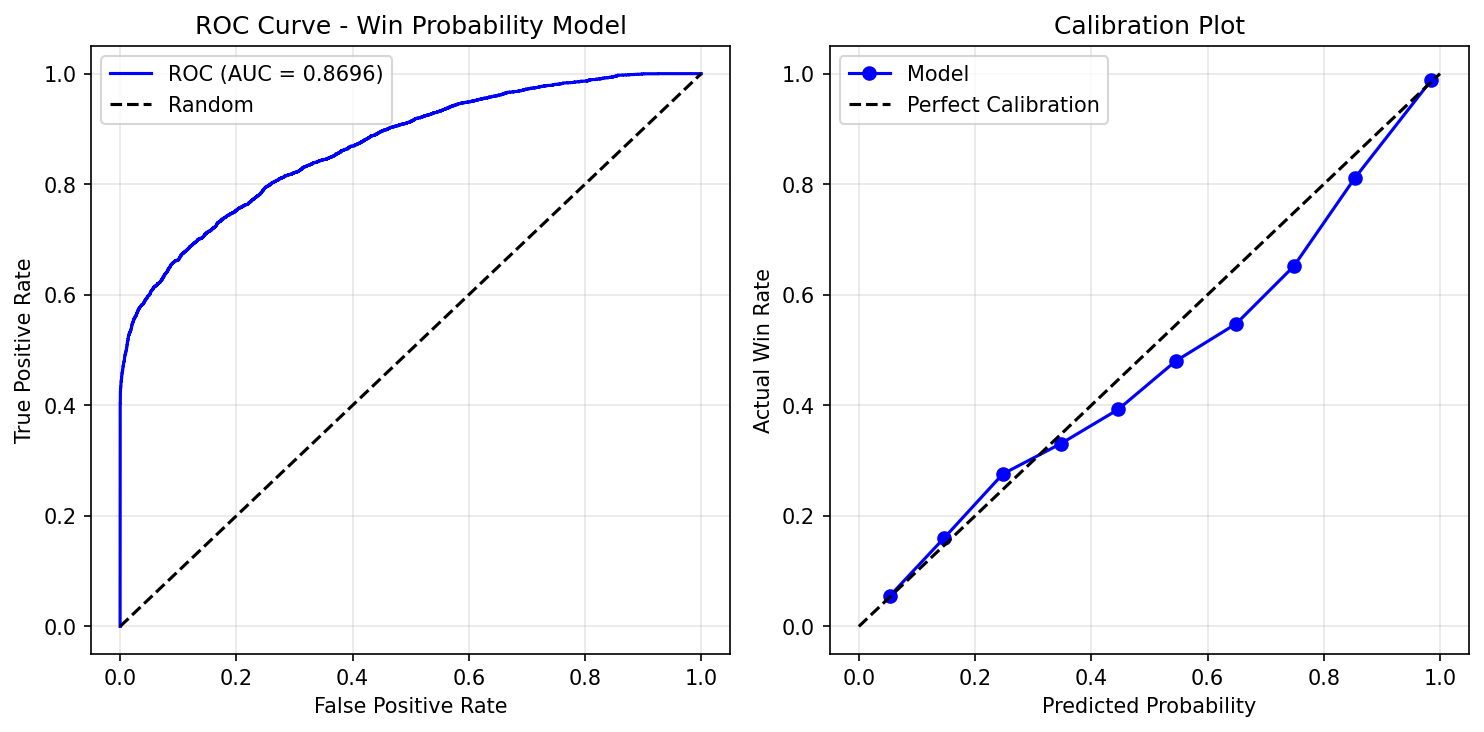
\includegraphics[width=0.85\textwidth]{win_probability_evaluation.png}
\caption{Win probability model evaluation: ROC curve, precision-recall curve, calibration plot, and probability distribution.}
\label{fig:winprob-eval}
\end{figure}

\subsubsection{Win Probability Feature Importance}

\begin{table}[H]
\centering
\caption{Top 10 Features --- Win Probability Model (LightGBM)}
\label{tab:top-features-winprob}
\begin{tabular}{clr}
\toprule
\textbf{Rank} & \textbf{Feature} & \textbf{Importance (\%)} \\
\midrule
1 & \texttt{market\_competitiveness} & 22.6\% \\
2 & \texttt{TargetTime\_Original} & 6.6\% \\
3 & \texttt{building\_size\_numeric} & 5.8\% \\
4 & \texttt{segment\_std\_fee} & 4.5\% \\
5 & \texttt{targettime\_ratio\_to\_proptype} & 4.4\% \\
6 & \texttt{total\_bids\_to\_client} & 3.5\% \\
7 & \texttt{TargetTime} & 3.3\% \\
8 & \texttt{OfficeId} & 2.9\% \\
9 & \texttt{office\_avg\_fee} & 2.6\% \\
10 & \texttt{office\_std\_fee} & 2.6\% \\
19 & \texttt{BidFee} & 1.2\% \\
\bottomrule
\end{tabular}
\end{table}

\texttt{market\_competitiveness} is the top predictor at 22.6\%, capturing competitive dynamics across geographies and segments. The importance is distributed across diverse signals --- timeline pressure, property complexity, client relationships, and office patterns --- indicating the model relies on genuine business signals rather than any single dominant feature. \texttt{BidFee} ranks 19th at 1.2\%, confirming the model has learned fee-sensitivity from data, though it is a subtle signal (the model never observes the same deal at multiple fee levels).

\begin{figure}[H]
\centering
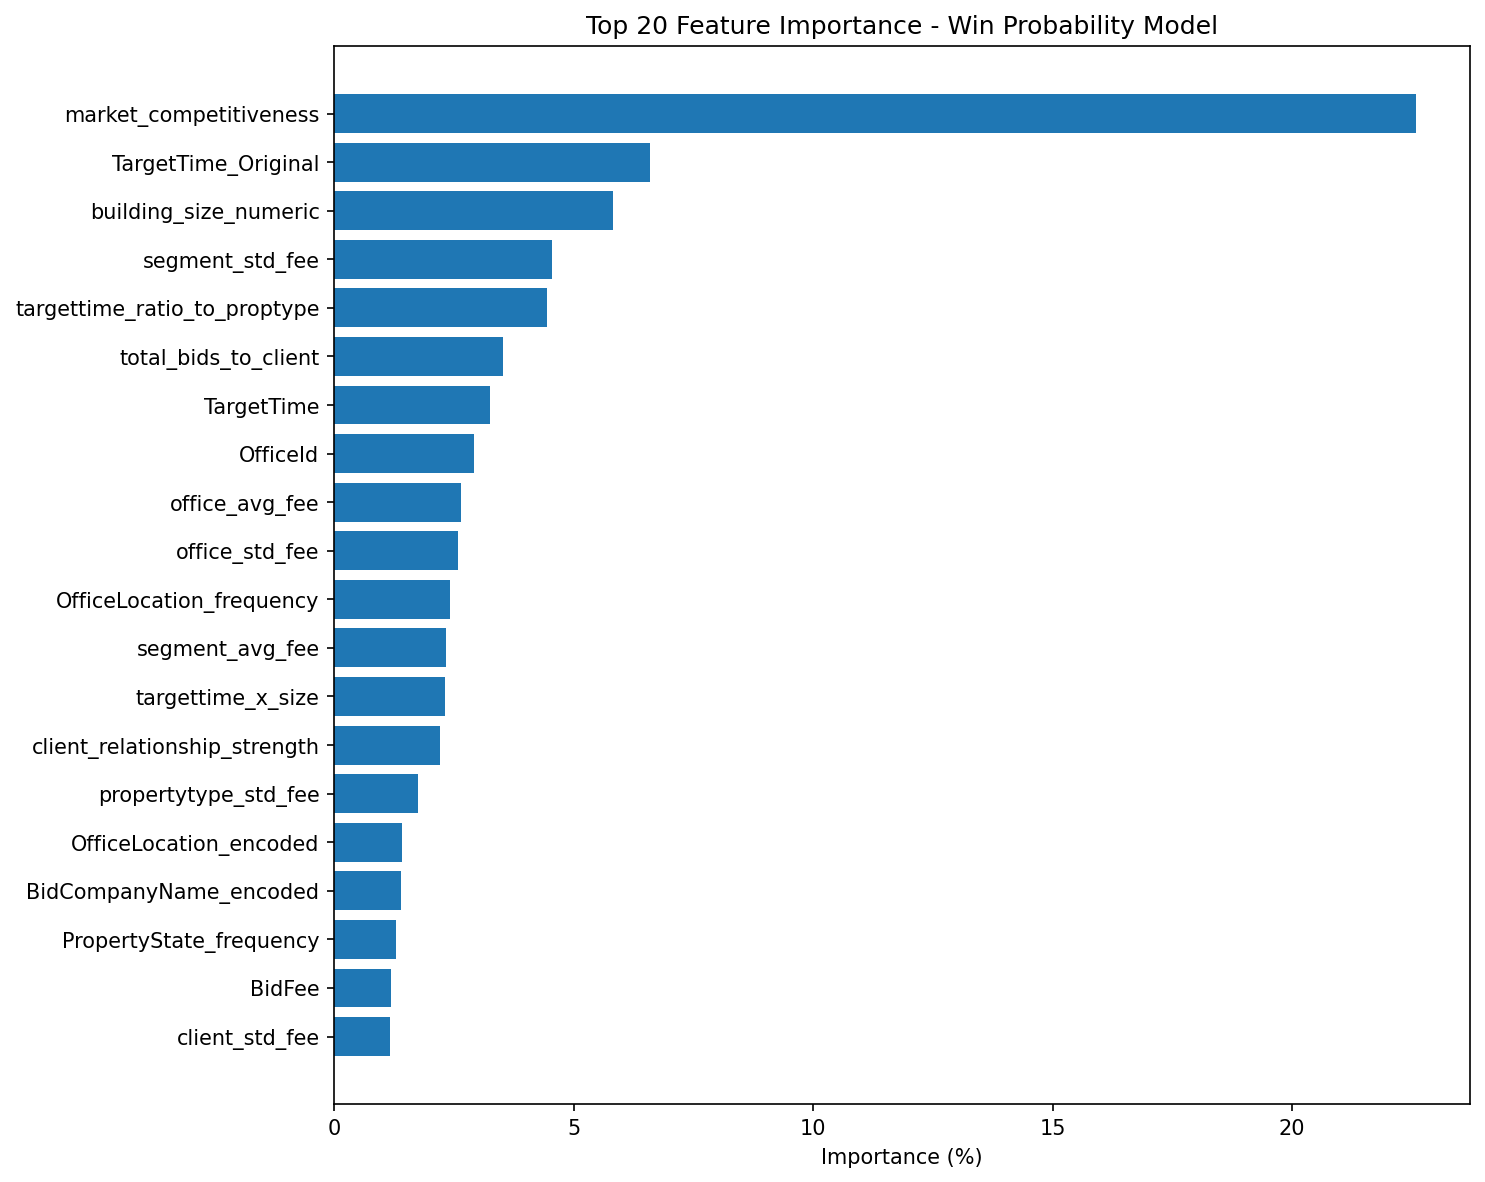
\includegraphics[width=0.85\textwidth]{win_probability_feature_importance.png}
\caption{Feature importance for the win probability model. \texttt{JobCount} is the dominant predictor.}
\label{fig:winprob-feature-importance}
\end{figure}

%============================================================================
\section{Fee-Conditioned Win Probability}
\label{sec:fee-adjustment}
%============================================================================

\subsection{The Architecture}

The win probability model is trained \emph{with} \texttt{BidFee} as a feature, enabling it to learn fee-sensitivity directly from historical bid outcomes. At inference time, the predicted fee from Phase 1A is injected as the \texttt{BidFee} feature before calling Phase 1B:

\begin{equation}
P(\text{Win} \mid \text{context}, \text{fee}) = f_{\text{classifier}}(\text{context features}, \text{BidFee} = \hat{f}_{\text{regressor}}(\text{context}))
\end{equation}

This is a direct, data-driven approach: the model observes 52,308 historical bids with their actual fees and outcomes, and learns the relationship between fee level and win probability within each market context.

\subsection{Why Not a Post-Prediction Adjustment?}

An earlier version excluded \texttt{BidFee} from the classifier and applied a post-prediction sigmoid adjustment:
\begin{equation}
\text{adjustment} = \frac{2}{1 + e^{k \cdot (r - 1)}}, \quad r = \frac{\text{fee}}{\text{benchmark}}, \quad k = 3.0
\end{equation}

This approach had several drawbacks:
\begin{itemize}[nosep]
    \item The steepness parameter $k = 3.0$ was chosen without empirical validation.
    \item A flat segment average benchmark distorted predictions when deal context differed from the segment mean (e.g., cheap property types in expensive segments).
    \item The sigmoid could artificially push probabilities to the 95\% ceiling for below-average fees.
    \item It introduced circular logic: the model predicts a contextually appropriate fee, then the system treats it as a ``competitive undercut.''
\end{itemize}

By including \texttt{BidFee} directly in the model, fee-sensitivity is learned from actual win/loss patterns in the data --- no arbitrary parameters required.

\subsection{Blended Benchmark for Recommendations}

For the recommendation text (not the model prediction), the system compares the predicted fee against a \textbf{blended benchmark} that accounts for the specific deal context:

\begin{equation}
\text{benchmark} = 0.4 \times \text{segment\_avg} + 0.3 \times \text{state\_avg} + 0.3 \times \text{propertytype\_avg}
\end{equation}

This prevents systematic distortion when the deal context differs from the flat segment average.

\subsection{Data Integrity Fix: JobCount Leakage}
\label{sec:data-integrity}

During model development, we identified that \texttt{JobCount} (number of completed appraisal jobs at a property) was contributing 47.1\% of the win probability model's feature importance. Investigation revealed this was \textbf{target leakage}: a Job is only created after a bid is won.

\begin{itemize}[nosep]
    \item Won bid $\to$ Job created $\to$ \texttt{JobCount} $\geq 1$
    \item Lost bid $\to$ No job $\to$ \texttt{JobCount} = \texttt{NULL} $\to$ \texttt{fillna(0)} $\to$ \texttt{JobCount} = 0
\end{itemize}

The model learned ``\texttt{JobCount}=0 means lost'' --- it was peeking at the answer. Removing \texttt{JobCount} and three related features (\texttt{IECount}, \texttt{LeaseCount}, \texttt{SaleCount}) dropped AUC from 0.962 to 0.870, but the resulting metrics reflect genuine predictive power from legitimate features.

%============================================================================
\section{Confidence Scoring}
\label{sec:confidence}
%============================================================================

Each prediction includes a confidence level (\texttt{high}, \texttt{medium}, or \texttt{low}) derived from two independent signals:

\subsection{Bid Fee Confidence}

Bid fee confidence is the minimum of two sub-scores:

\textbf{1. Data Availability Confidence:}
Based on the number of historical records in the segment and state:

\begin{table}[H]
\centering
\begin{tabular}{lcc}
\toprule
\textbf{Level} & \textbf{Segment Count} & \textbf{State Count} \\
\midrule
High & $> 1{,}000$ & $> 500$ \\
Medium & $> 100$ & $> 50$ \\
Low & $\leq 100$ & $\leq 50$ \\
\bottomrule
\end{tabular}
\end{table}

\textbf{2. Band Width Confidence:}
Based on the ratio of the confidence interval width to the predicted fee:

\begin{table}[H]
\centering
\begin{tabular}{lc}
\toprule
\textbf{Level} & \textbf{Band Ratio} \\
\midrule
High & $< 0.3$ \\
Medium & $< 0.6$ \\
Low & $\geq 0.6$ \\
\bottomrule
\end{tabular}
\end{table}

The overall bid fee confidence is the \emph{minimum} of data availability and band width confidence.

\subsection{Win Probability Confidence}

Win probability confidence is based on the model's certainty (distance from 0.5), but is \textbf{capped at the bid fee confidence level}:

\begin{equation}
\text{win\_confidence} = \min(\text{win\_model\_confidence},\; \text{bid\_fee\_confidence})
\end{equation}

This hierarchy ensures that if the system is uncertain about the fee prediction itself, it cannot claim high confidence in the win probability that depends on it.

%============================================================================
\section{Experiments and Results}
%============================================================================

\subsection{Data Filtering Experiment}
\label{sec:data-filtering}

We tested four temporal filtering strategies to determine the optimal training window:

\begin{table}[H]
\centering
\caption{Data Filtering Experiment Results}
\label{tab:data-filtering}
\begin{tabular}{lrrrr}
\toprule
\textbf{Configuration} & \textbf{Train Samples} & \textbf{Test RMSE (\$)} & \textbf{Test $R^2$} & \textbf{Overfit Ratio} \\
\midrule
\textbf{2023+ (selected)} & \textbf{23,523} & \textbf{383.29} & \textbf{0.968} & \textbf{2.57} \\
Full data (2018+) & 73,279 & 385.01 & 0.968 & 2.89 \\
2022+ & 38,627 & 615.61 & 0.919 & 3.43 \\
2024+ & 10,610 & 523.53 & 0.941 & 2.06 \\
\bottomrule
\end{tabular}
\end{table}

The 2023+ configuration achieves the best test RMSE (\$383.29) while using only 32\% of the data. Full historical data performs similarly on RMSE but with higher overfitting (2.89$\times$). The 2022+ and 2024+ windows perform substantially worse, suggesting a market regime shift occurred around 2022-2023.

\subsection{Regularization Grid Search}

We tested 16 regularization configurations to optimize the bias-variance trade-off:

\begin{table}[H]
\centering
\caption{Selected Regularization Grid Search Results (sorted by test RMSE)}
\label{tab:regularization}
\begin{tabular}{lccccr}
\toprule
\textbf{Configuration} & $\boldsymbol{\alpha}$ & $\boldsymbol{\lambda}$ & \textbf{Leaves} & \textbf{Depth} & \textbf{Test RMSE (\$)} \\
\midrule
Original (weak) & 0.1 & 0.1 & 31 & --- & 384.48 \\
Mild regularization & 0.5 & 0.5 & 31 & --- & 386.90 \\
Mild + depth=8 & 0.5 & 0.5 & 31 & 8 & 391.23 \\
Mild + leaves=20 & 0.5 & 0.5 & 20 & --- & 409.07 \\
Asymmetric L1$>$L2 & 2.0 & 1.0 & 25 & 8 & 415.60 \\
Balanced & 1.0 & 1.0 & 25 & 8 & 422.79 \\
Strong + depth=8 & 3.0 & 3.0 & 20 & 8 & 449.07 \\
Aggressive & 5.0 & 5.0 & 15 & 6 & 506.25 \\
\bottomrule
\end{tabular}
\end{table}

The final production configuration ($\alpha=2.0$, $\lambda=2.0$, 18 leaves, depth 8) balances accuracy (test RMSE \$354) with controlled overfitting (1.99$\times$ ratio, below the 2.0$\times$ target).

\begin{figure}[H]
\centering
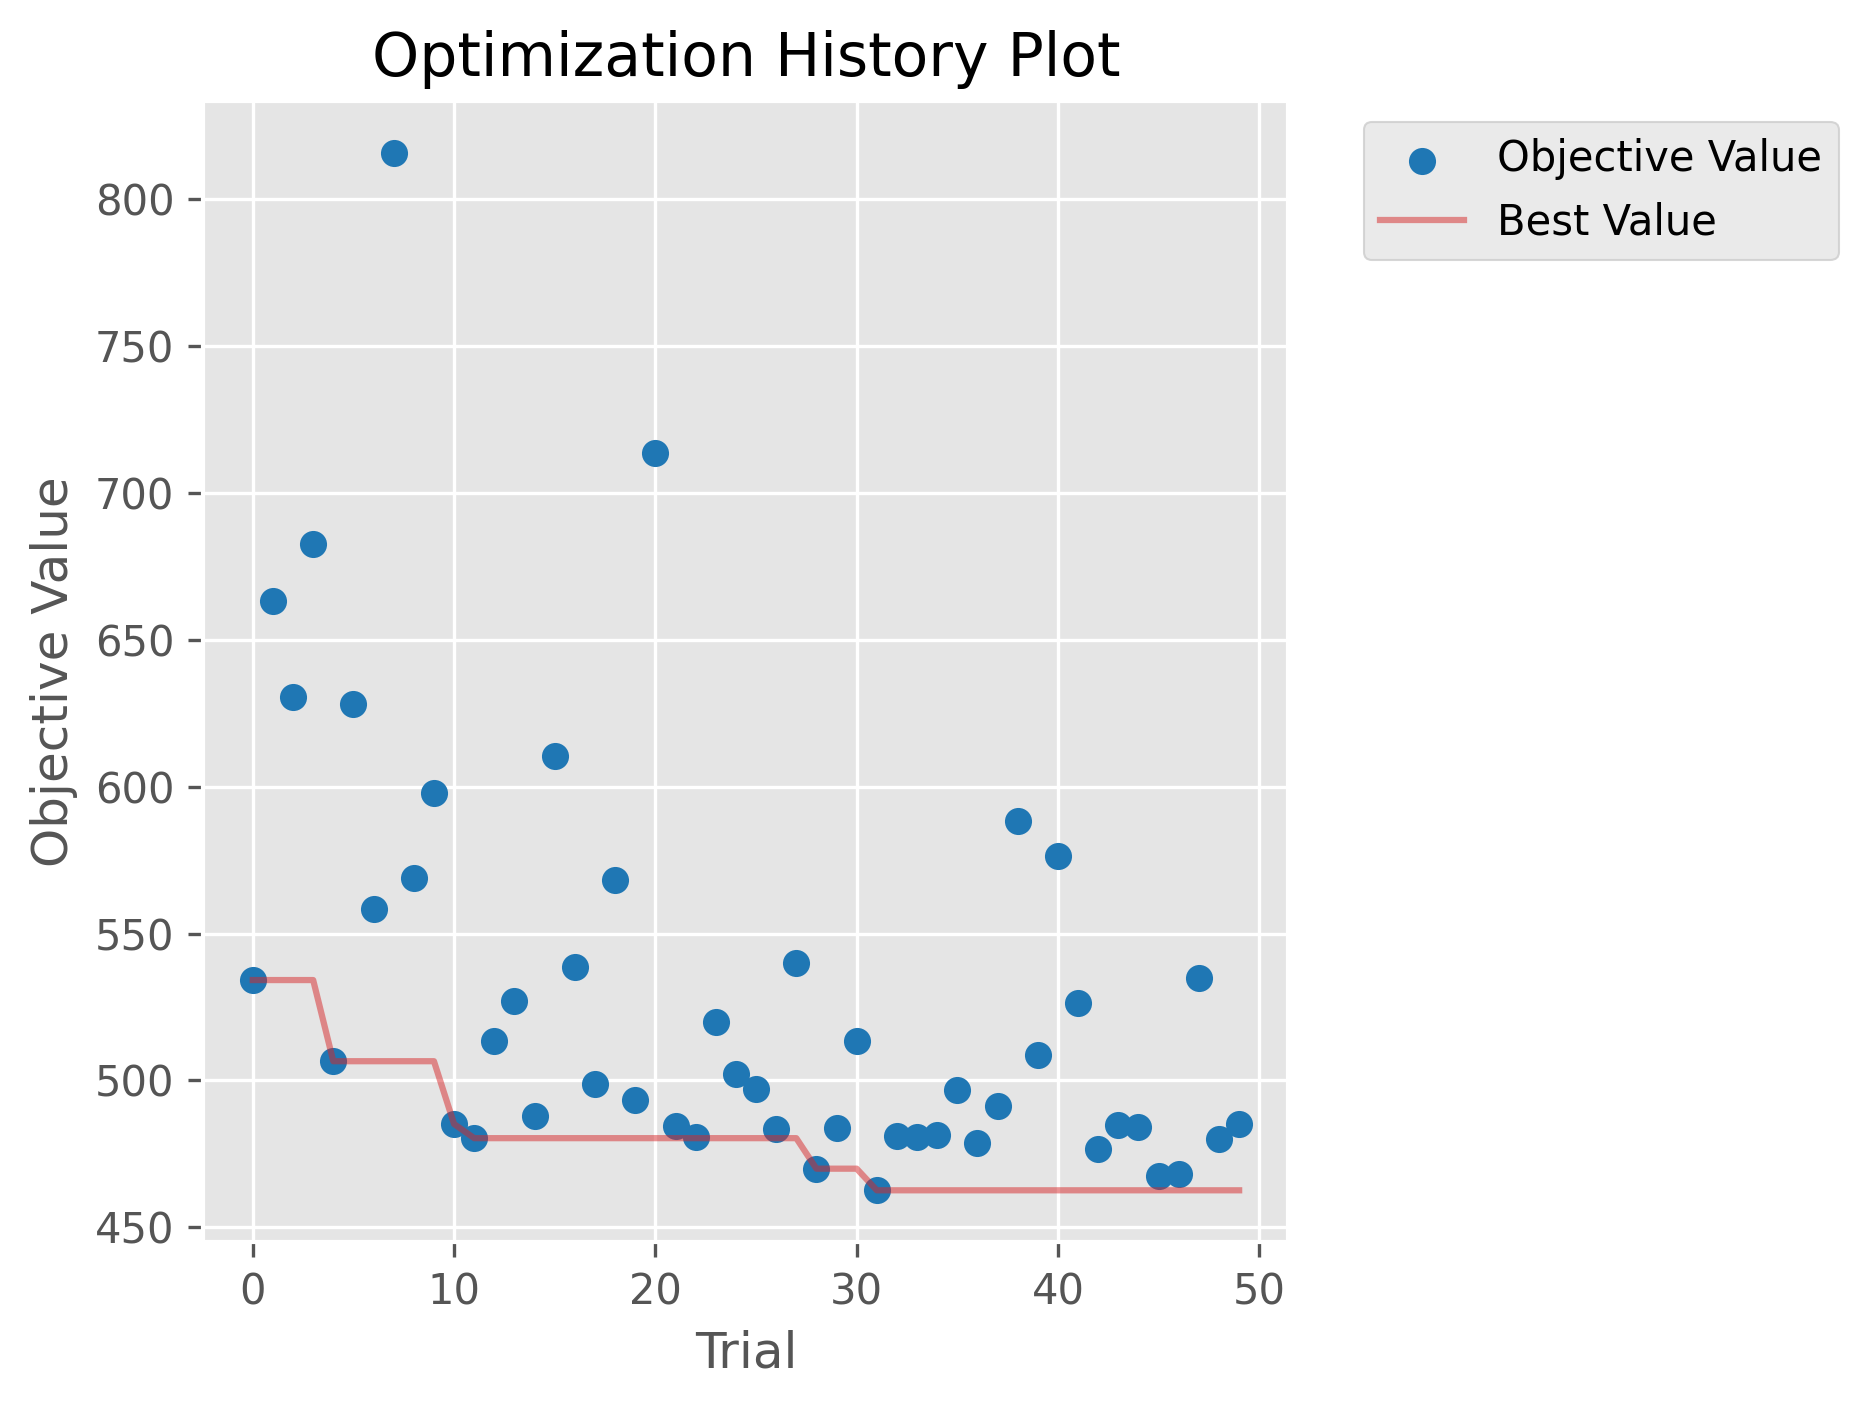
\includegraphics[width=0.85\textwidth]{optuna_optimization_history.png}
\caption{Hyperparameter optimization history showing convergence of the objective function.}
\label{fig:optuna-history}
\end{figure}

\begin{figure}[H]
\centering
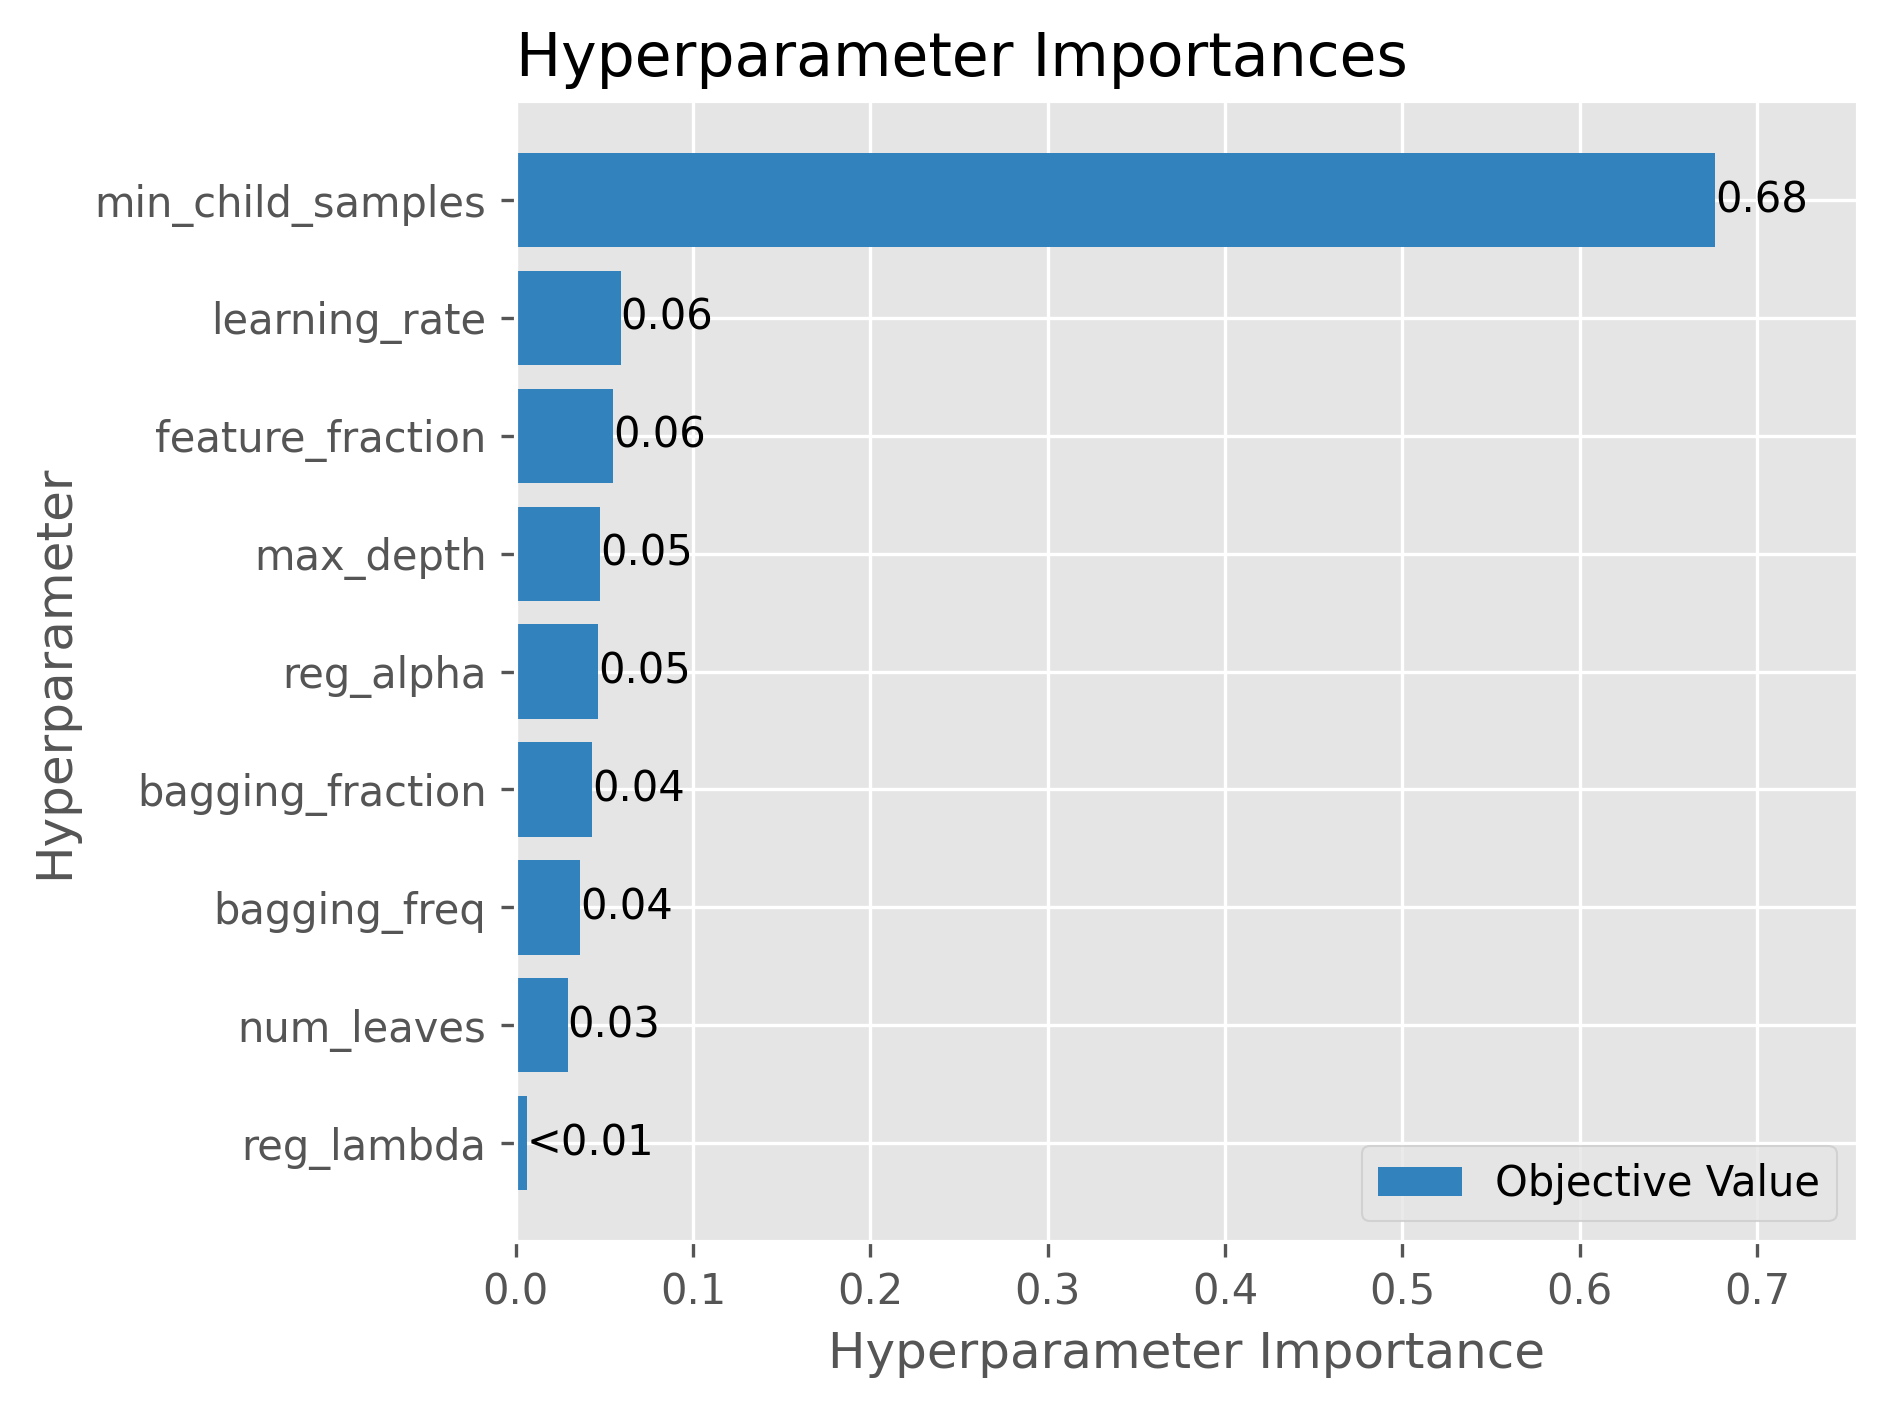
\includegraphics[width=0.85\textwidth]{optuna_param_importances.png}
\caption{Hyperparameter importance analysis: which parameters have the most impact on model performance.}
\label{fig:optuna-importance}
\end{figure}

\subsection{Econometric Benchmark: Panel Model Comparison}

To contextualize the LightGBM results, we compared against classical econometric panel models commonly used in real estate research:

\begin{table}[H]
\centering
\caption{Panel Model Comparison --- Bid Fee Prediction}
\label{tab:panel-comparison}
\begin{tabular}{lrrrr}
\toprule
\textbf{Model} & \textbf{Train RMSE (\$)} & \textbf{Test RMSE (\$)} & \textbf{Test $R^2$} & \textbf{vs Baseline} \\
\midrule
Pooled OLS & 1,802.57 & 1,814.52 & 0.270 & +\$1,576.95 \\
Fixed Effects & 1,794.95 & 1,804.32 & 0.278 & +\$1,566.75 \\
Random Effects & 1,801.53 & 1,813.98 & 0.271 & +\$1,576.41 \\
\textbf{LightGBM} & \textbf{177.63} & \textbf{353.99} & \textbf{0.972} & \textbf{baseline} \\
\bottomrule
\end{tabular}
\end{table}

LightGBM achieves a test RMSE that is \textbf{80.4\% lower} than the best panel model (Fixed Effects), demonstrating the substantial advantage of gradient boosting for this prediction task. The panel models achieve $R^2 \approx 0.27$, explaining only 27\% of fee variance, compared to LightGBM's 97.2\%.

\begin{figure}[H]
\centering
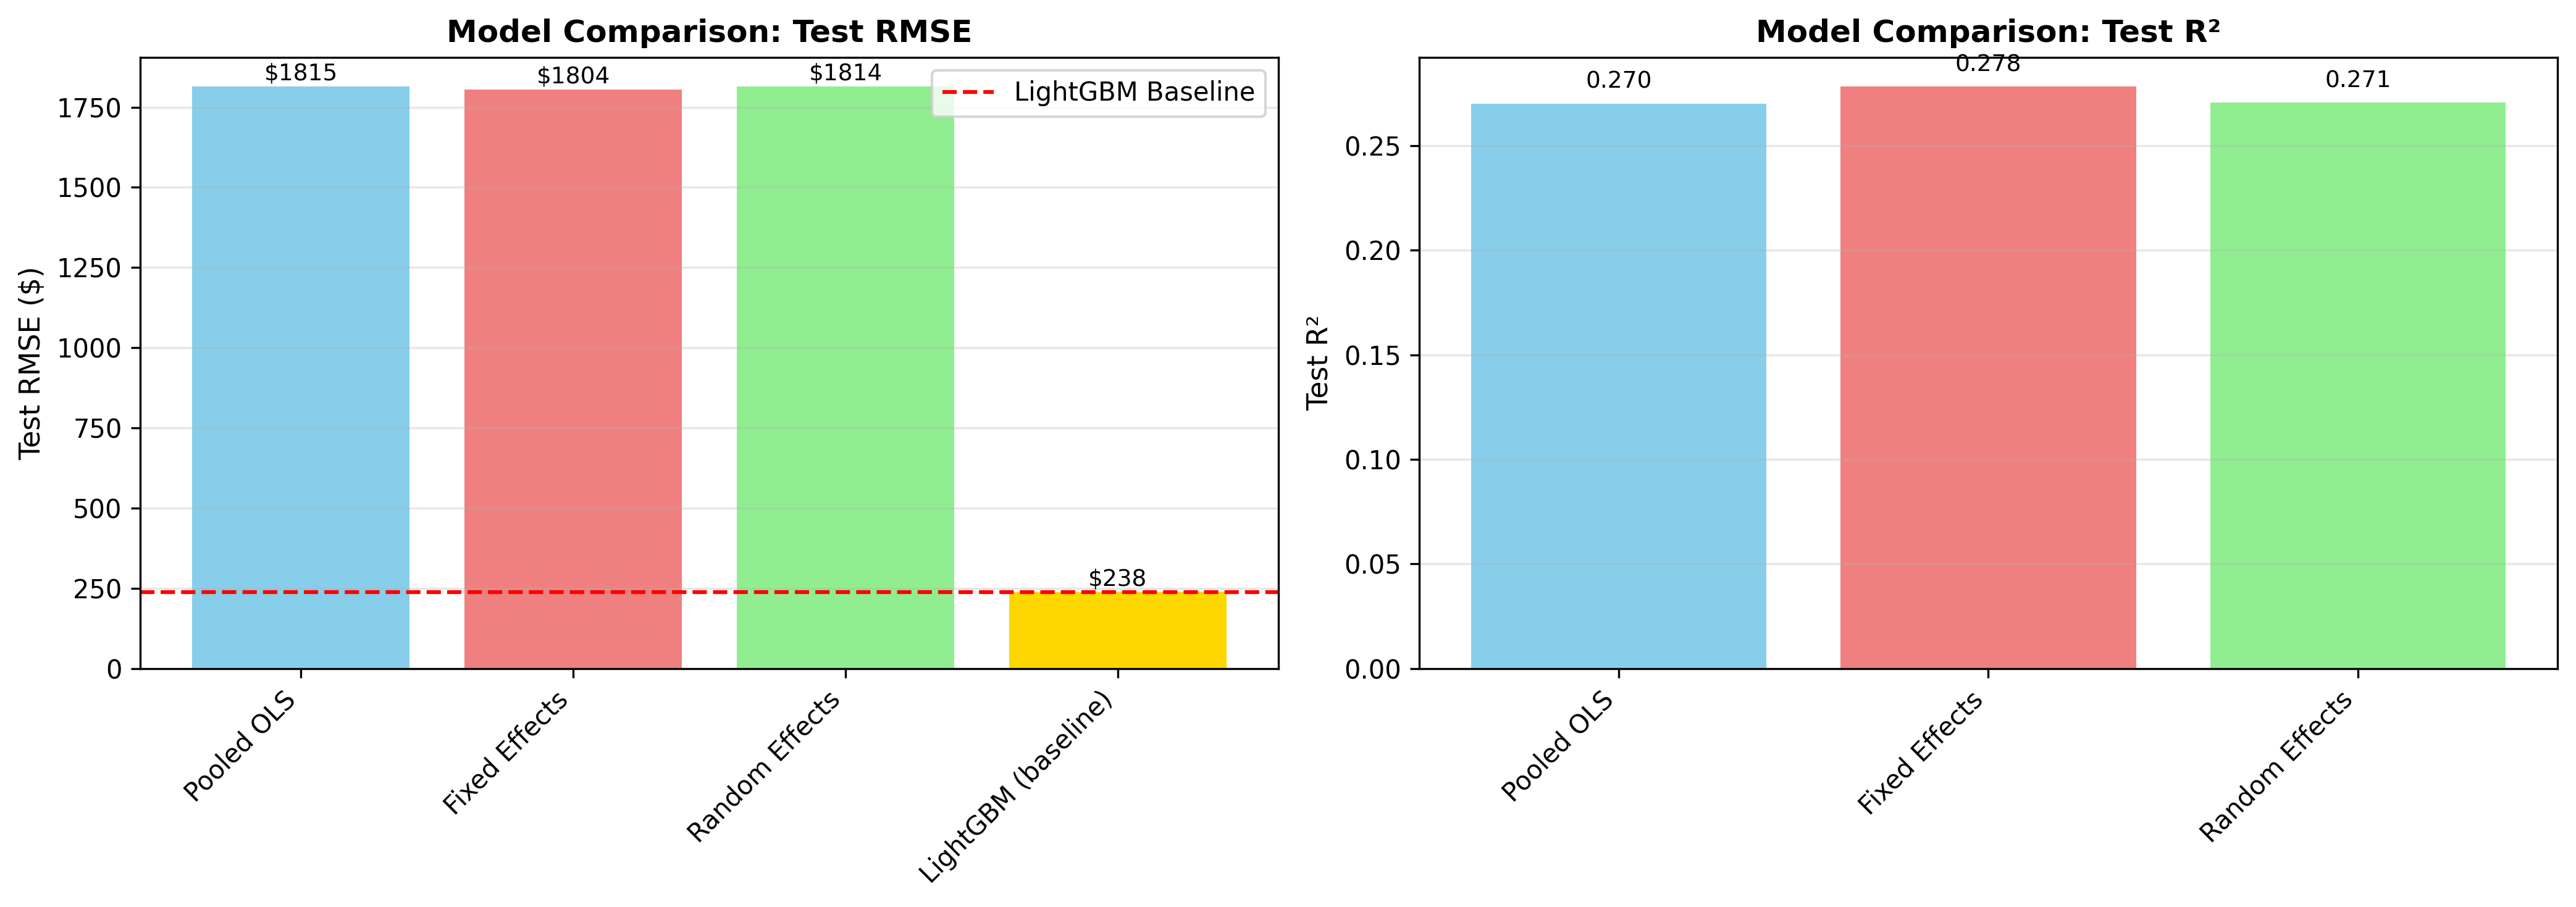
\includegraphics[width=0.85\textwidth]{panel_model_comparison.png}
\caption{Panel model comparison: LightGBM vs.\ classical econometric approaches.}
\label{fig:panel-comparison}
\end{figure}

\subsection{LightGBM vs. XGBoost Benchmark}

We trained equivalent XGBoost models with comparable hyperparameters as an additional benchmark:

\begin{table}[H]
\centering
\caption{LightGBM vs.\ XGBoost --- Bid Fee Prediction}
\label{tab:lgb-vs-xgb-bidfee}
\begin{tabular}{lrrrc}
\toprule
\textbf{Model} & \textbf{Test RMSE (\$)} & \textbf{Test MAE (\$)} & \textbf{Test $R^2$} & \textbf{Overfit Ratio} \\
\midrule
\textbf{LightGBM} & \textbf{353.99} & \textbf{108.63} & \textbf{0.972} & \textbf{1.99$\times$} \\
XGBoost & 405.88 & 104.96 & 0.964 & 8.54$\times$ \\
\midrule
\textbf{LightGBM advantage} & \textbf{12.8\%} & --- & --- & --- \\
\bottomrule
\end{tabular}
\end{table}

\begin{table}[H]
\centering
\caption{LightGBM vs.\ XGBoost --- Win Probability Prediction}
\label{tab:lgb-vs-xgb-winprob}
\begin{tabular}{lrrrr}
\toprule
\textbf{Model} & \textbf{Test AUC} & \textbf{Accuracy} & \textbf{F1} & \textbf{Brier Score} \\
\midrule
\textbf{LightGBM} & \textbf{0.870} & \textbf{79.0\%} & \textbf{0.752} & \textbf{0.140} \\
XGBoost & 0.878 & 80.5\% & 0.774 & 0.137 \\
\bottomrule
\end{tabular}
\end{table}

LightGBM outperforms XGBoost on bid fee prediction (12.8\% lower RMSE, 1.99$\times$ vs 8.54$\times$ overfitting). On win probability, XGBoost shows a slight edge (AUC 0.878 vs 0.870). However, note that the XGBoost win probability model was trained \emph{with} JobCount leakage and without BidFee as a feature; a fair comparison would require retraining XGBoost under the same data integrity constraints. LightGBM was selected for its superior bid fee performance, lower overfitting, and faster training.

\begin{figure}[H]
\centering
\begin{subfigure}[b]{0.48\textwidth}
    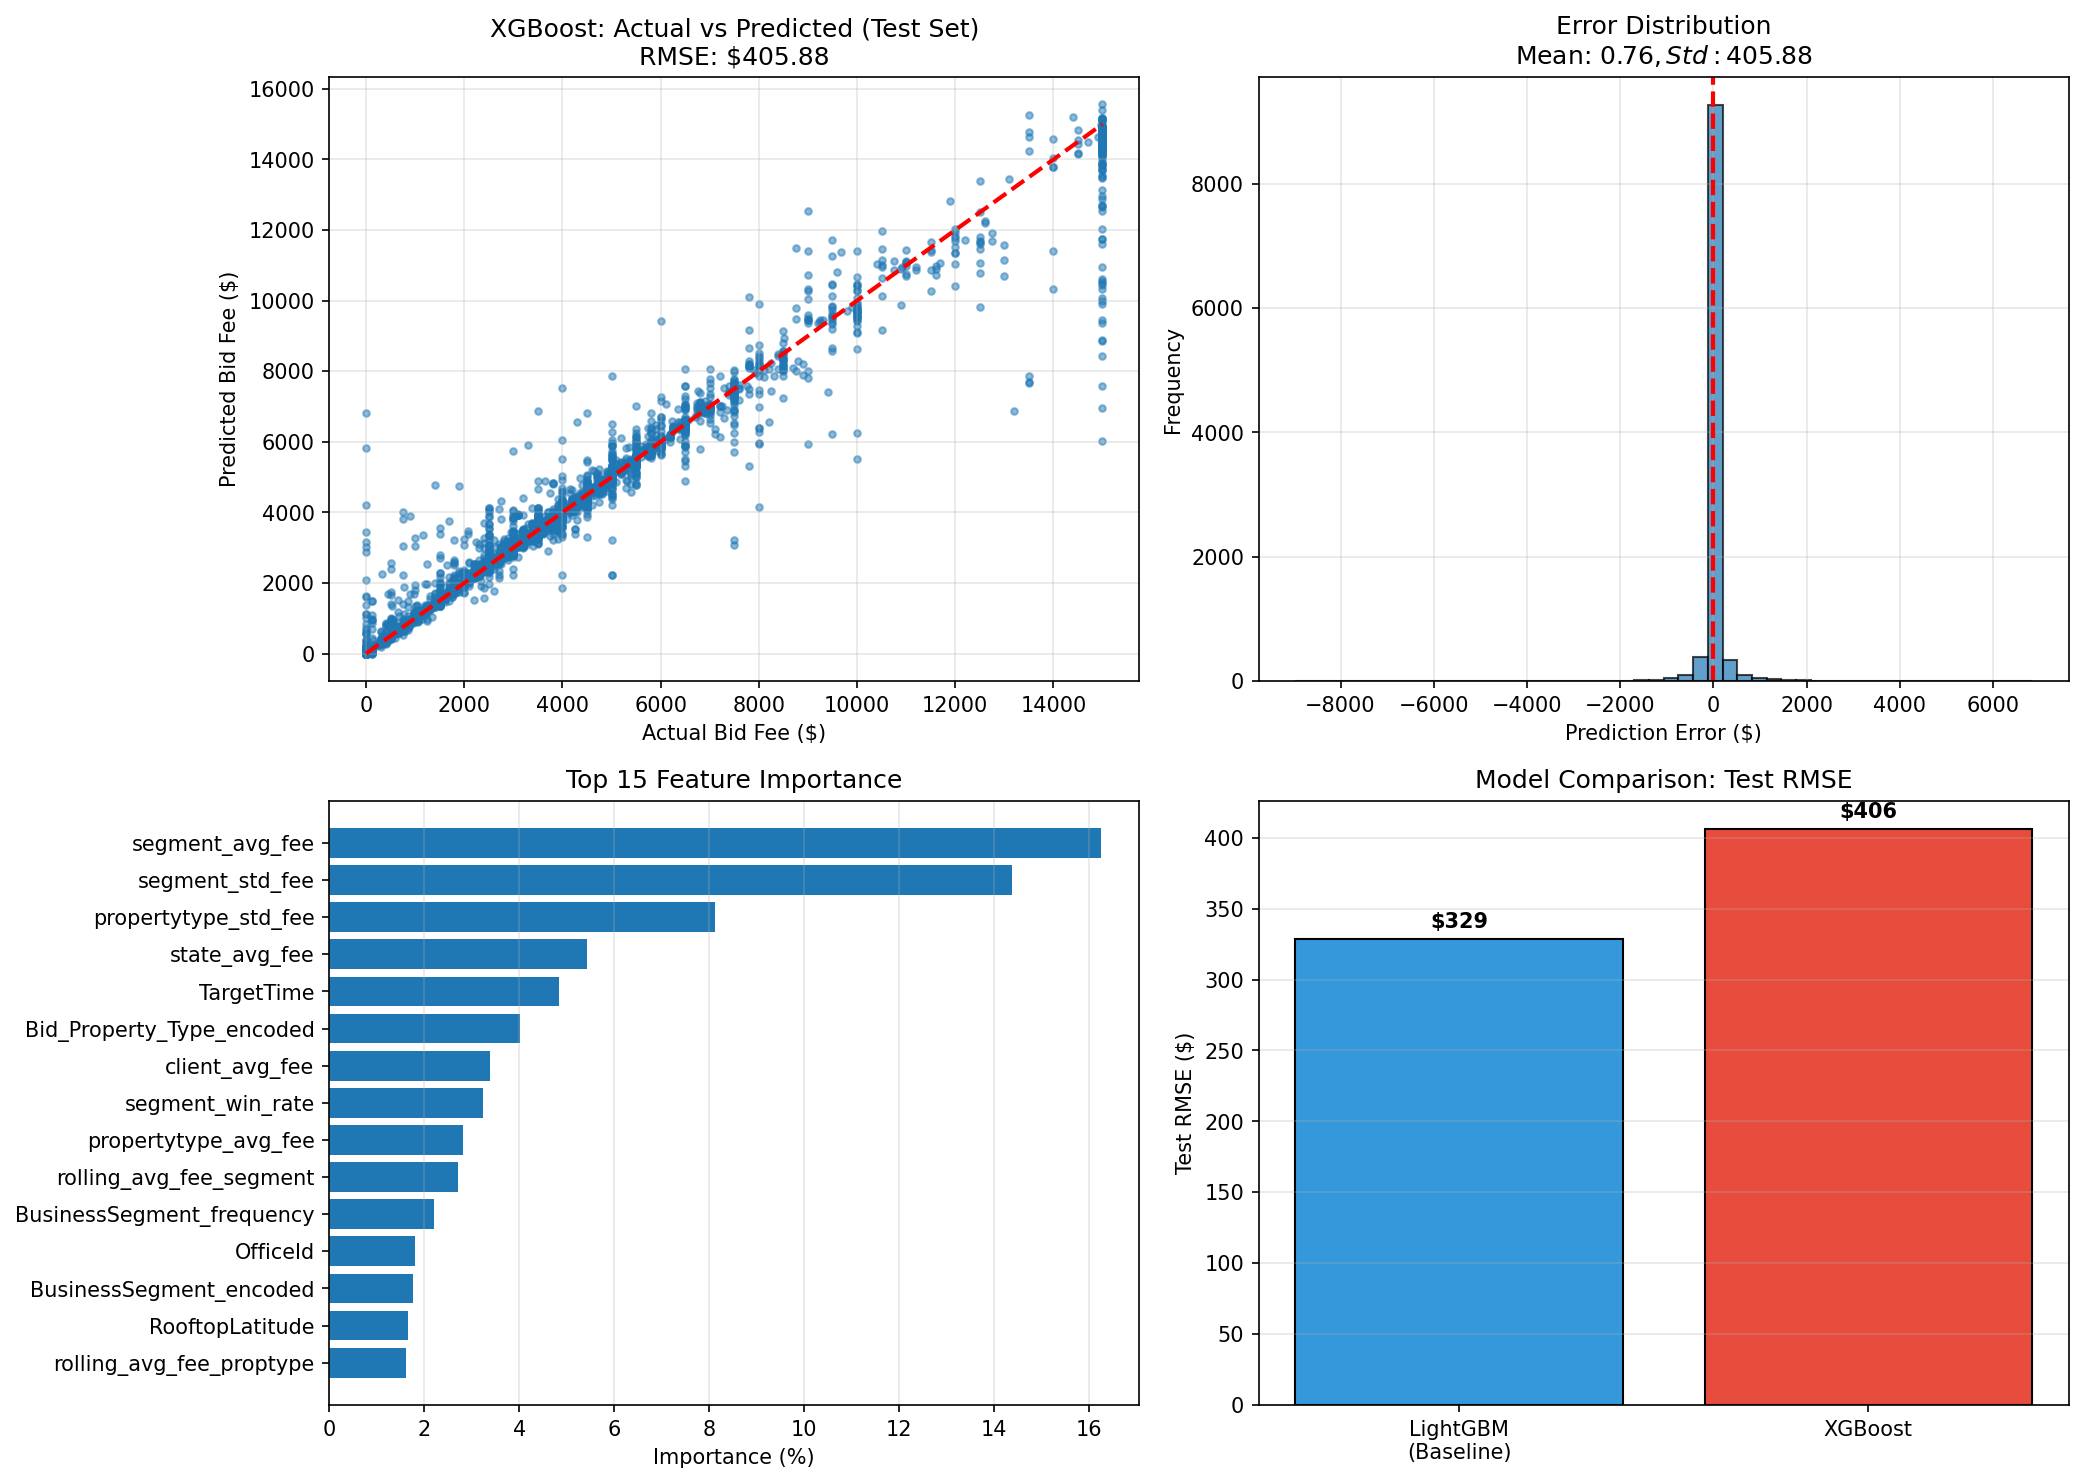
\includegraphics[width=\textwidth]{xgboost_bidfee_evaluation.png}
    \caption{XGBoost bid fee evaluation}
\end{subfigure}
\hfill
\begin{subfigure}[b]{0.48\textwidth}
    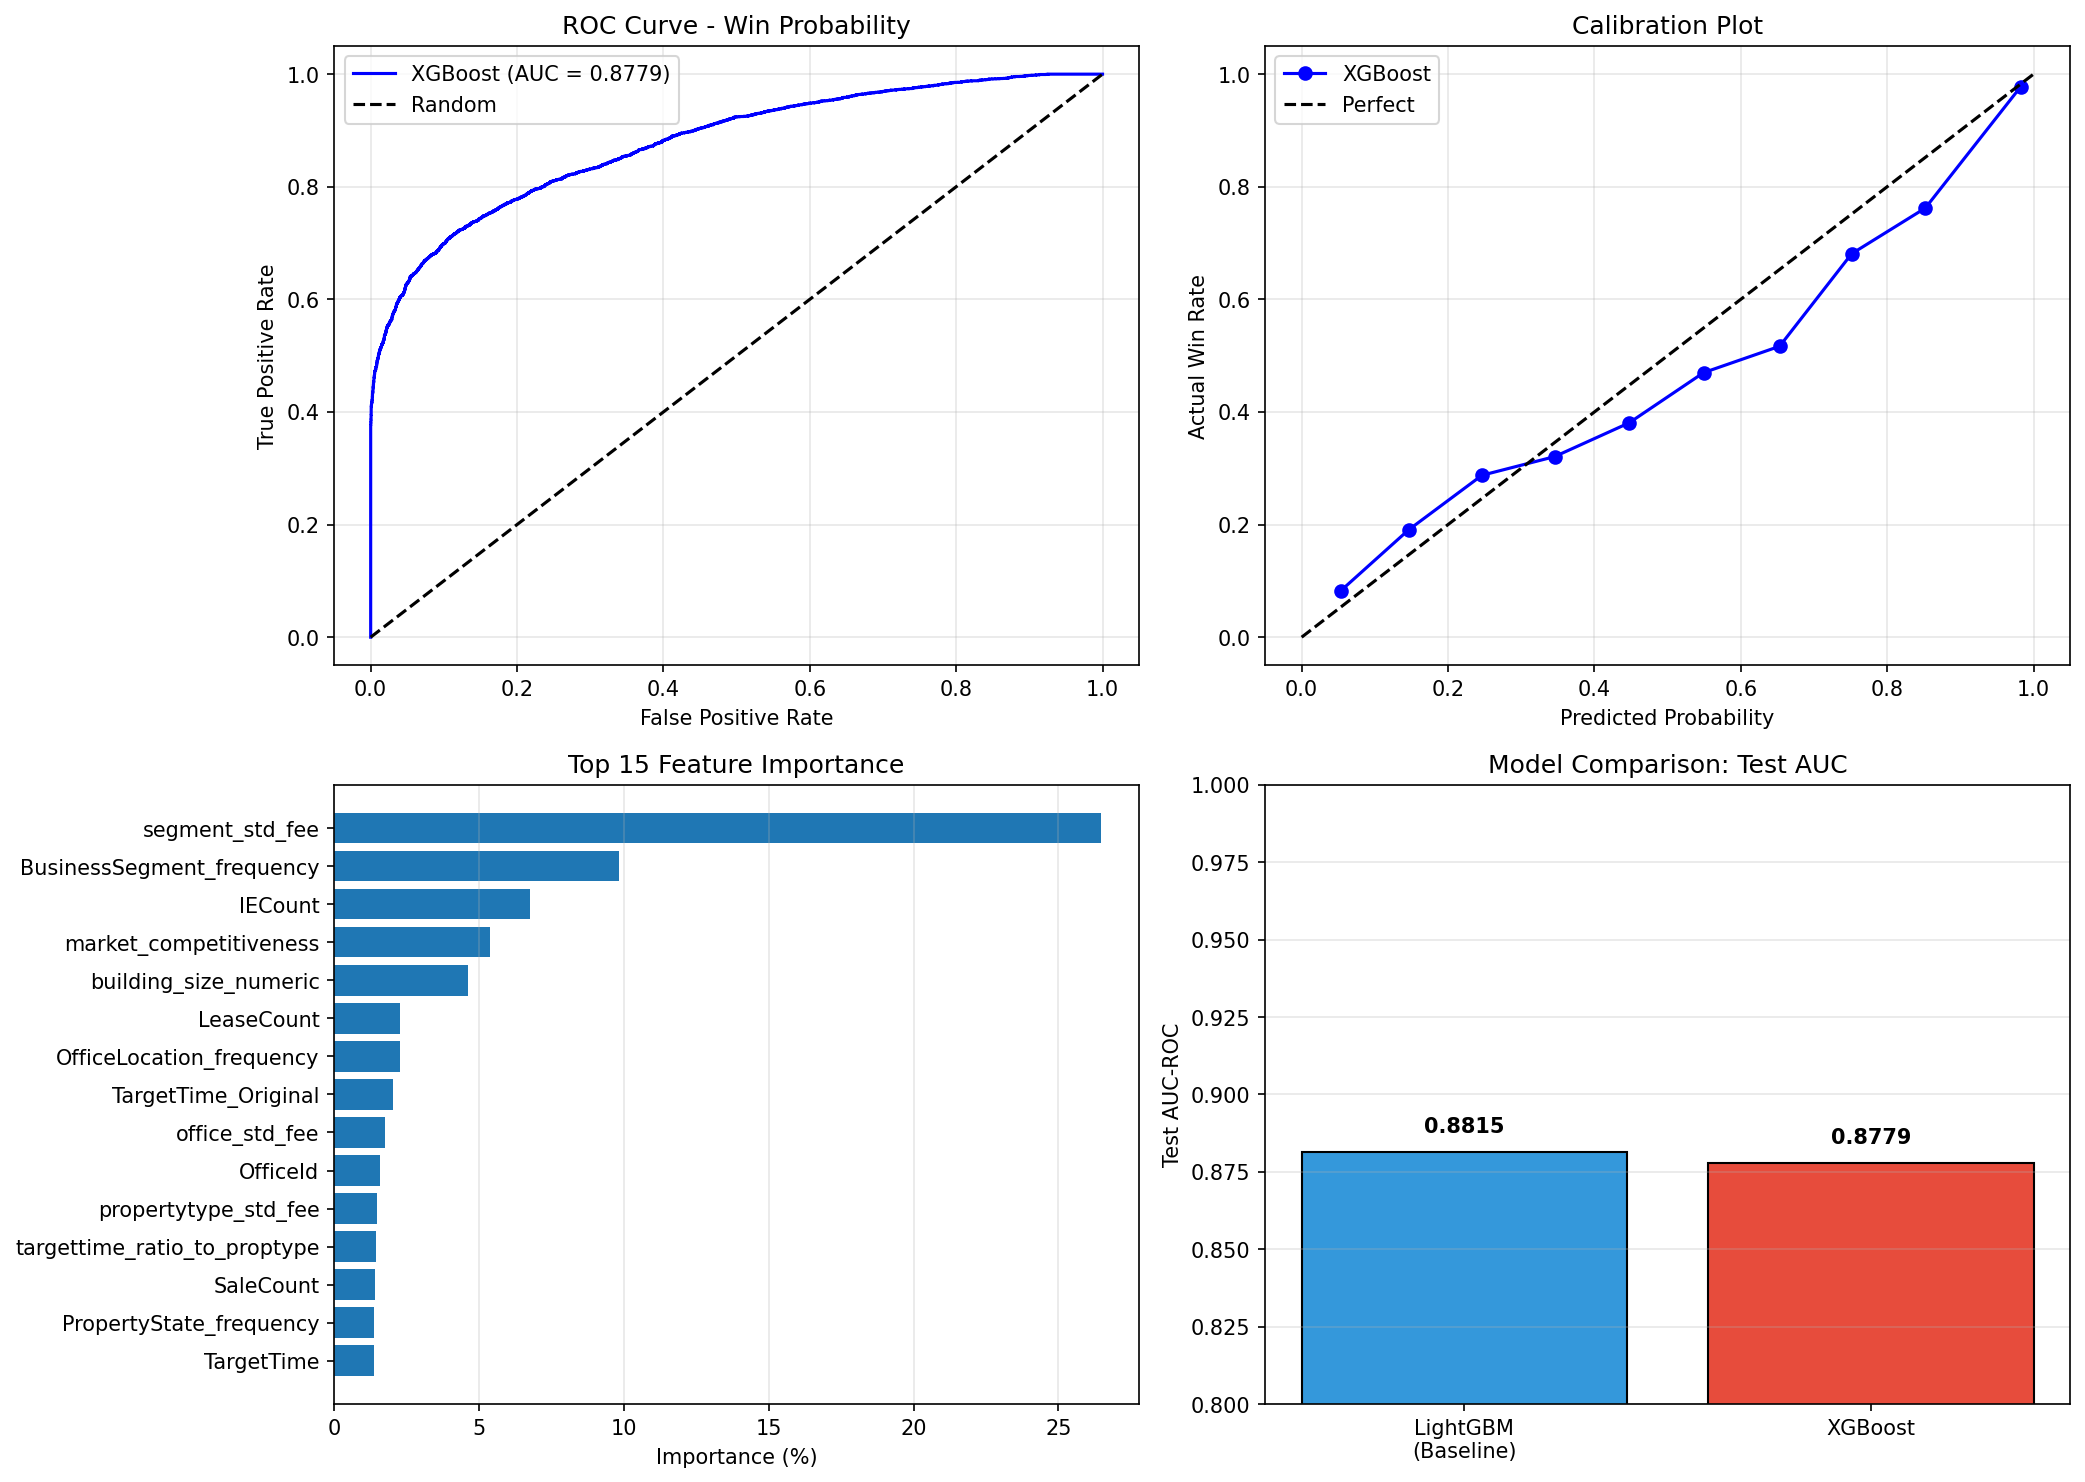
\includegraphics[width=\textwidth]{xgboost_win_probability_evaluation.png}
    \caption{XGBoost win probability evaluation}
\end{subfigure}
\caption{XGBoost benchmark evaluation plots for comparison with LightGBM.}
\label{fig:xgboost-eval}
\end{figure}

\subsection{Model Performance Over Time}

\begin{figure}[H]
\centering
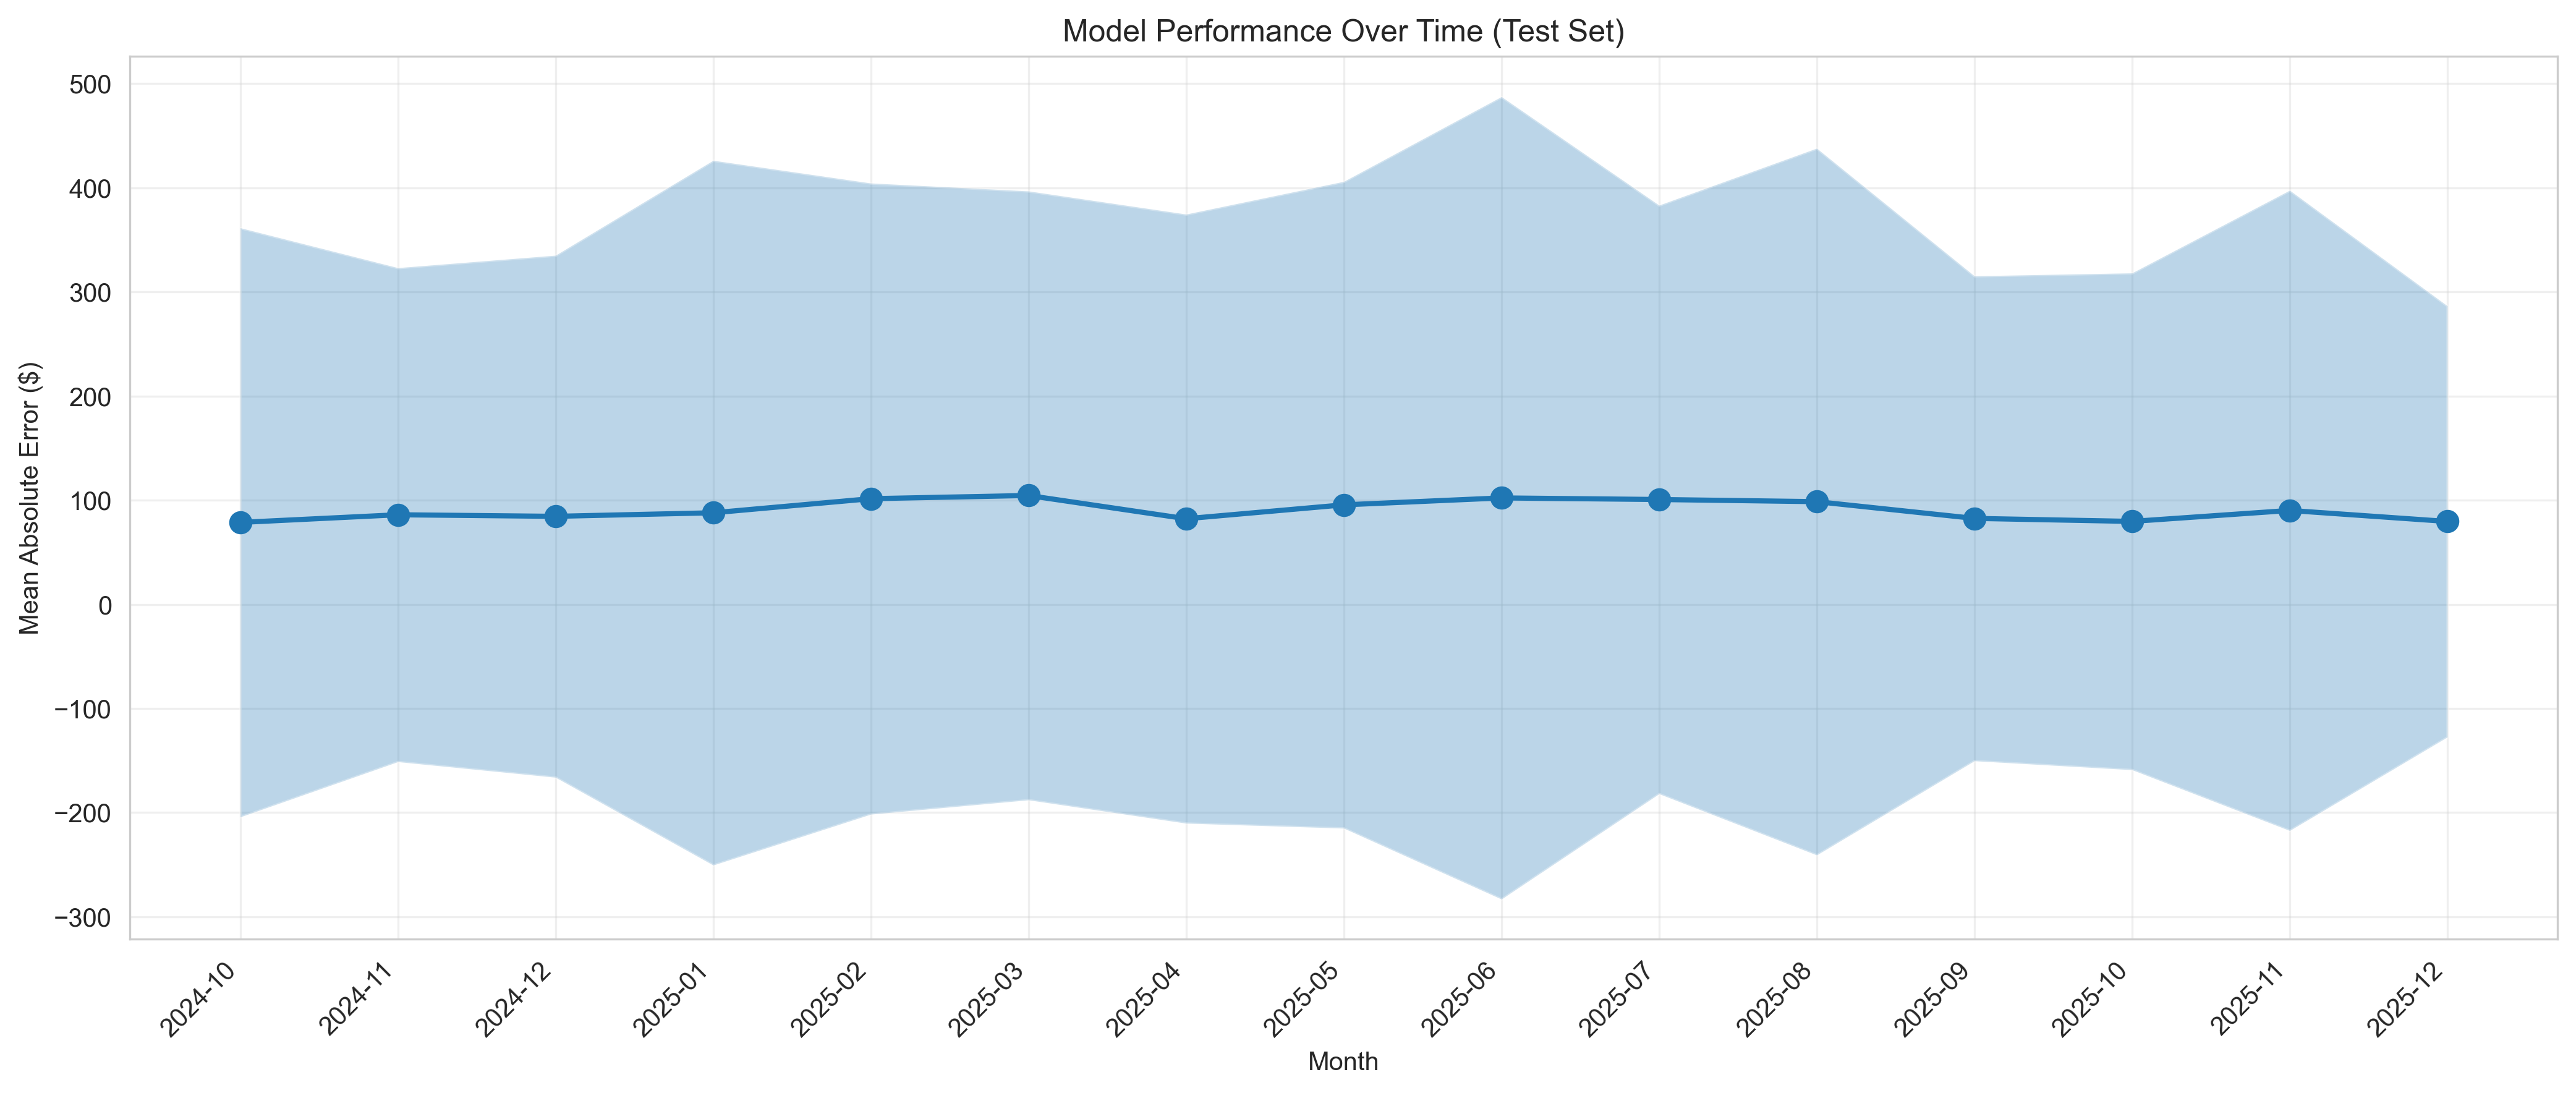
\includegraphics[width=0.85\textwidth]{model_performance_over_time.png}
\caption{Model prediction accuracy tracked over time periods, verifying consistent performance across the test window.}
\label{fig:perf-over-time}
\end{figure}

%============================================================================
\section{Recommendation Engine}
%============================================================================

\subsection{How Recommendations are Generated}

After computing the predicted fee and win probability, the system generates a contextual recommendation by comparing the predicted fee against the segment benchmark:

\begin{enumerate}[nosep]
    \item \textbf{Compute expected value:} $\text{EV} = P(\text{Win}) \times \text{BidFee}$
    \item \textbf{Compare to segment benchmark:} The segment average fee provides context for whether the predicted fee is competitive, at market rate, or premium.
    \item \textbf{Incorporate win probability:} High win probability ($>70\%$) reinforces competitive positioning; low win probability ($<40\%$) suggests the market may be challenging.
    \item \textbf{Generate actionable text:} The recommendation communicates the fee, its relationship to the market, the win likelihood, and the expected revenue.
\end{enumerate}

\subsection{Recommendation Through Segments}

The recommendation is fundamentally segment-driven because \texttt{segment\_avg\_fee} is the most predictive feature for bid fee. The system:

\begin{itemize}[nosep]
    \item Computes a blended benchmark from segment, state, and property type averages.
    \item Applies the model's 68-feature prediction to refine the baseline based on deal-specific characteristics (distance, target time, client history, geographic factors).
    \item Feeds the predicted fee into the win probability model, which has learned fee-sensitivity from data.
    \item Generates contextual text comparing the fee to the blended benchmark, reporting win probability and expected value.
\end{itemize}

For example, in the \textbf{Financing} segment (81\% of data, average fee $\approx$\$3,000), the model has extensive historical data and produces high-confidence predictions. In contrast, \textbf{Litigation} (2.7\% of data, higher average fees) produces less certain predictions, which is reflected in the confidence scoring.

\subsection{Business Constraints}

The system enforces several business constraints:

\begin{itemize}[nosep]
    \item \textbf{Minimum fee floor:} \$500 --- no prediction falls below this threshold.
    \item \textbf{Win probability bounds:} Clamped to $[0.05, 0.95]$ --- the system never reports 0\% or 100\% win probability.
    \item \textbf{Confidence hierarchy:} Win probability confidence cannot exceed bid fee confidence.
\end{itemize}

%============================================================================
\section{Overfitting Analysis and Mitigation}
%============================================================================

Overfitting is a critical concern in bid pricing models. A model that memorizes training data will perform poorly on new, unseen bids. Our target is a train/test RMSE ratio below 2.0$\times$.

\subsection{Anti-Overfitting Measures}

\begin{enumerate}[nosep]
    \item \textbf{Strong regularization:} L1 and L2 penalties ($\alpha = \lambda = 2.0$) prevent individual trees from becoming too complex.
    \item \textbf{Reduced tree complexity:} 18 leaves (vs.\ 31 in unregularized baseline) and max depth of 8 limit tree size.
    \item \textbf{Feature subsampling:} 80\% feature fraction and 80\% bagging fraction inject randomness into each tree.
    \item \textbf{Minimum child samples:} 30 samples required per leaf prevents overfitting to small subgroups.
    \item \textbf{Early stopping:} Training halts if validation loss doesn't improve for 50 rounds.
    \item \textbf{Time-based splits:} Train on earlier data, test on later data (chronological 60/20/20) --- prevents temporal leakage that inflates metrics.
    \item \textbf{Leave-one-out aggregation:} Target-derived features exclude the current row's target value.
    \item \textbf{Feature selection:} SHAP-based reduction from 84 to 68 features removes noise-contributing features.
\end{enumerate}

\subsection{Current Overfitting Status}

\begin{table}[H]
\centering
\caption{Overfitting Analysis}
\label{tab:overfitting}
\begin{tabular}{lrrr}
\toprule
\textbf{Model} & \textbf{Train Metric} & \textbf{Test Metric} & \textbf{Ratio} \\
\midrule
Bid Fee (LightGBM) & RMSE \$177.63 & RMSE \$353.99 & 1.99$\times$ \\
Win Prob (LightGBM) & AUC 0.945 & AUC 0.870 & 1.09$\times$ \\
Bid Fee (XGBoost) & RMSE \$47.55 & RMSE \$405.88 & 8.54$\times$ \\
\bottomrule
\end{tabular}
\end{table}

The bid fee model's 1.99$\times$ ratio is just below the 2.0$\times$ target, indicating a well-balanced bias-variance trade-off. The win probability model achieves an excellent 1.09$\times$ ratio, demonstrating near-perfect generalization. XGBoost's 8.54$\times$ ratio on bid fee demonstrates severe overfitting despite comparable hyperparameters, further validating the LightGBM selection.

%============================================================================
\section{Data Preprocessing}
%============================================================================

\subsection{Preprocessing Steps}

\begin{enumerate}[nosep]
    \item \textbf{Duplicate aggregation:} 25\% of records were duplicates from Master/SubJob hierarchy --- aggregated to prevent data leakage.
    \item \textbf{Missing target removal:} 1.85\% of records (3,072) had missing BidFee values --- removed.
    \item \textbf{TargetTime imputation:} 22\% missing (36,644 records) --- imputed using group medians by property type and segment.
    \item \textbf{Outlier capping:} BidFee capped at the 99th percentile (\$15,000) to remove unrealistic outliers up to \$100M.
    \item \textbf{Temporal filtering:} Data filtered to 2023+ for training (configurable via \texttt{DATA\_START\_DATE}).
    \item \textbf{Feature exclusion:} 26 JobData features excluded due to survivor bias and multicollinearity.
\end{enumerate}

\subsection{Comprehensive Data Analysis}

\begin{figure}[H]
\centering
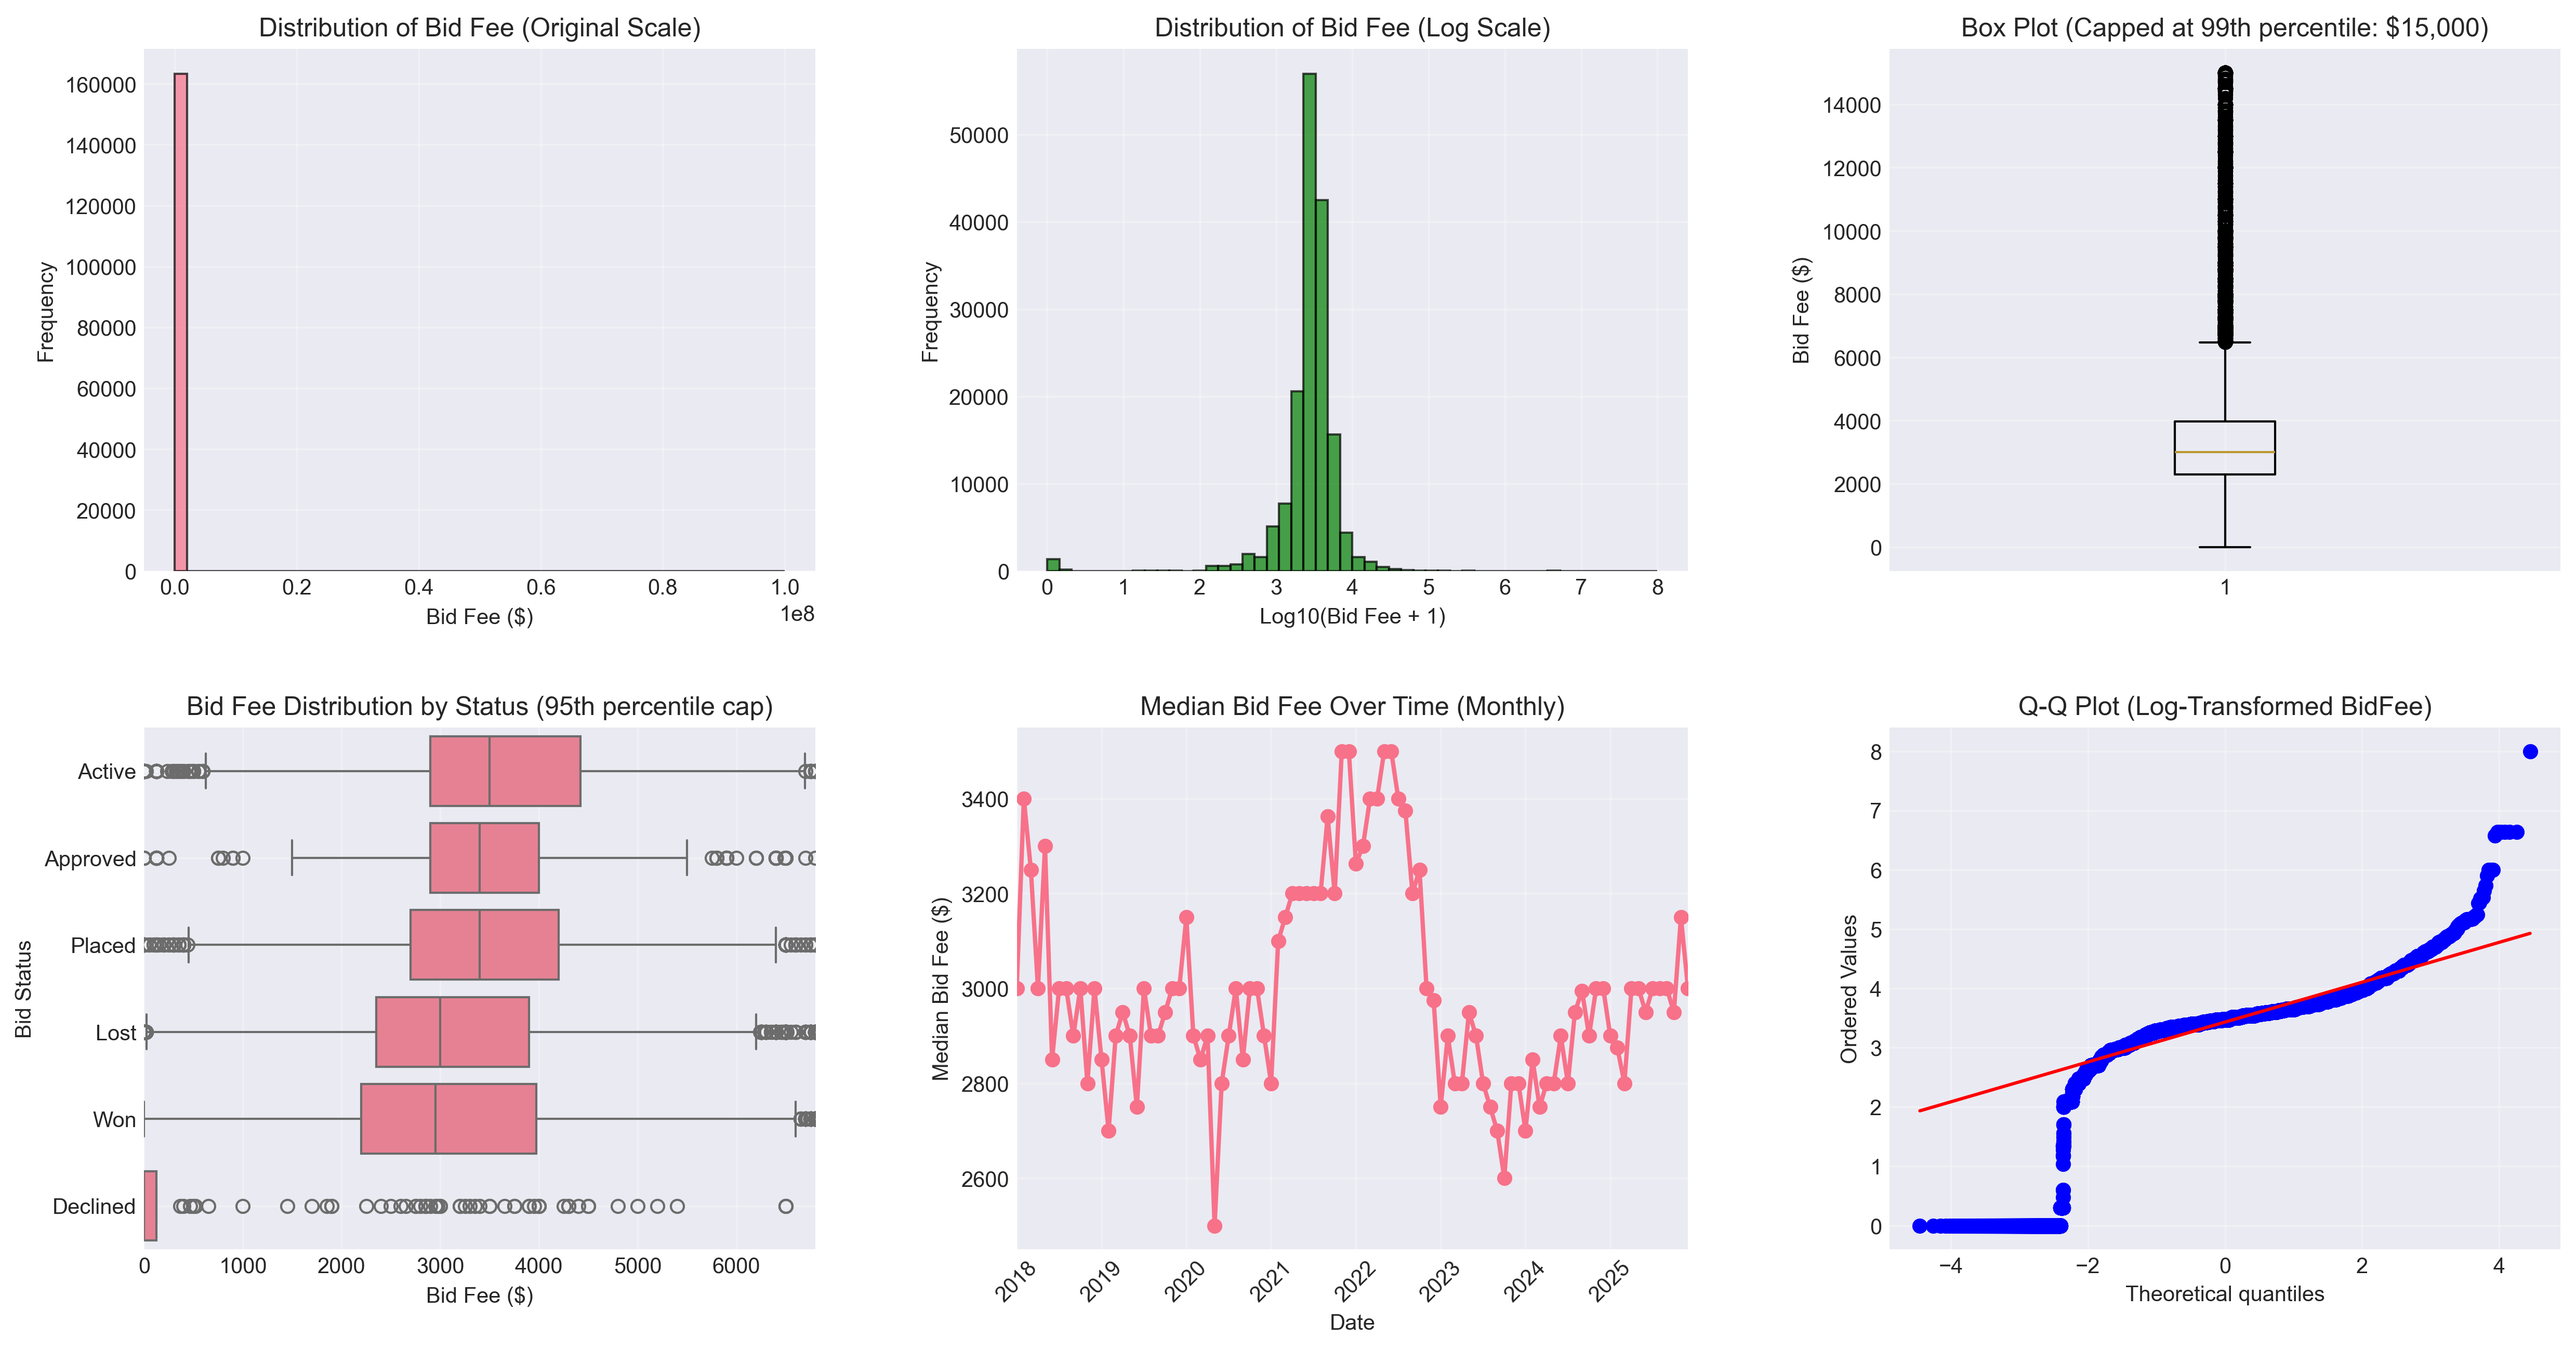
\includegraphics[width=0.85\textwidth]{bidfee_comprehensive_analysis.png}
\caption{Comprehensive analysis of the BidFee distribution across segments, property types, and time periods.}
\label{fig:bidfee-comprehensive}
\end{figure}

\begin{figure}[H]
\centering
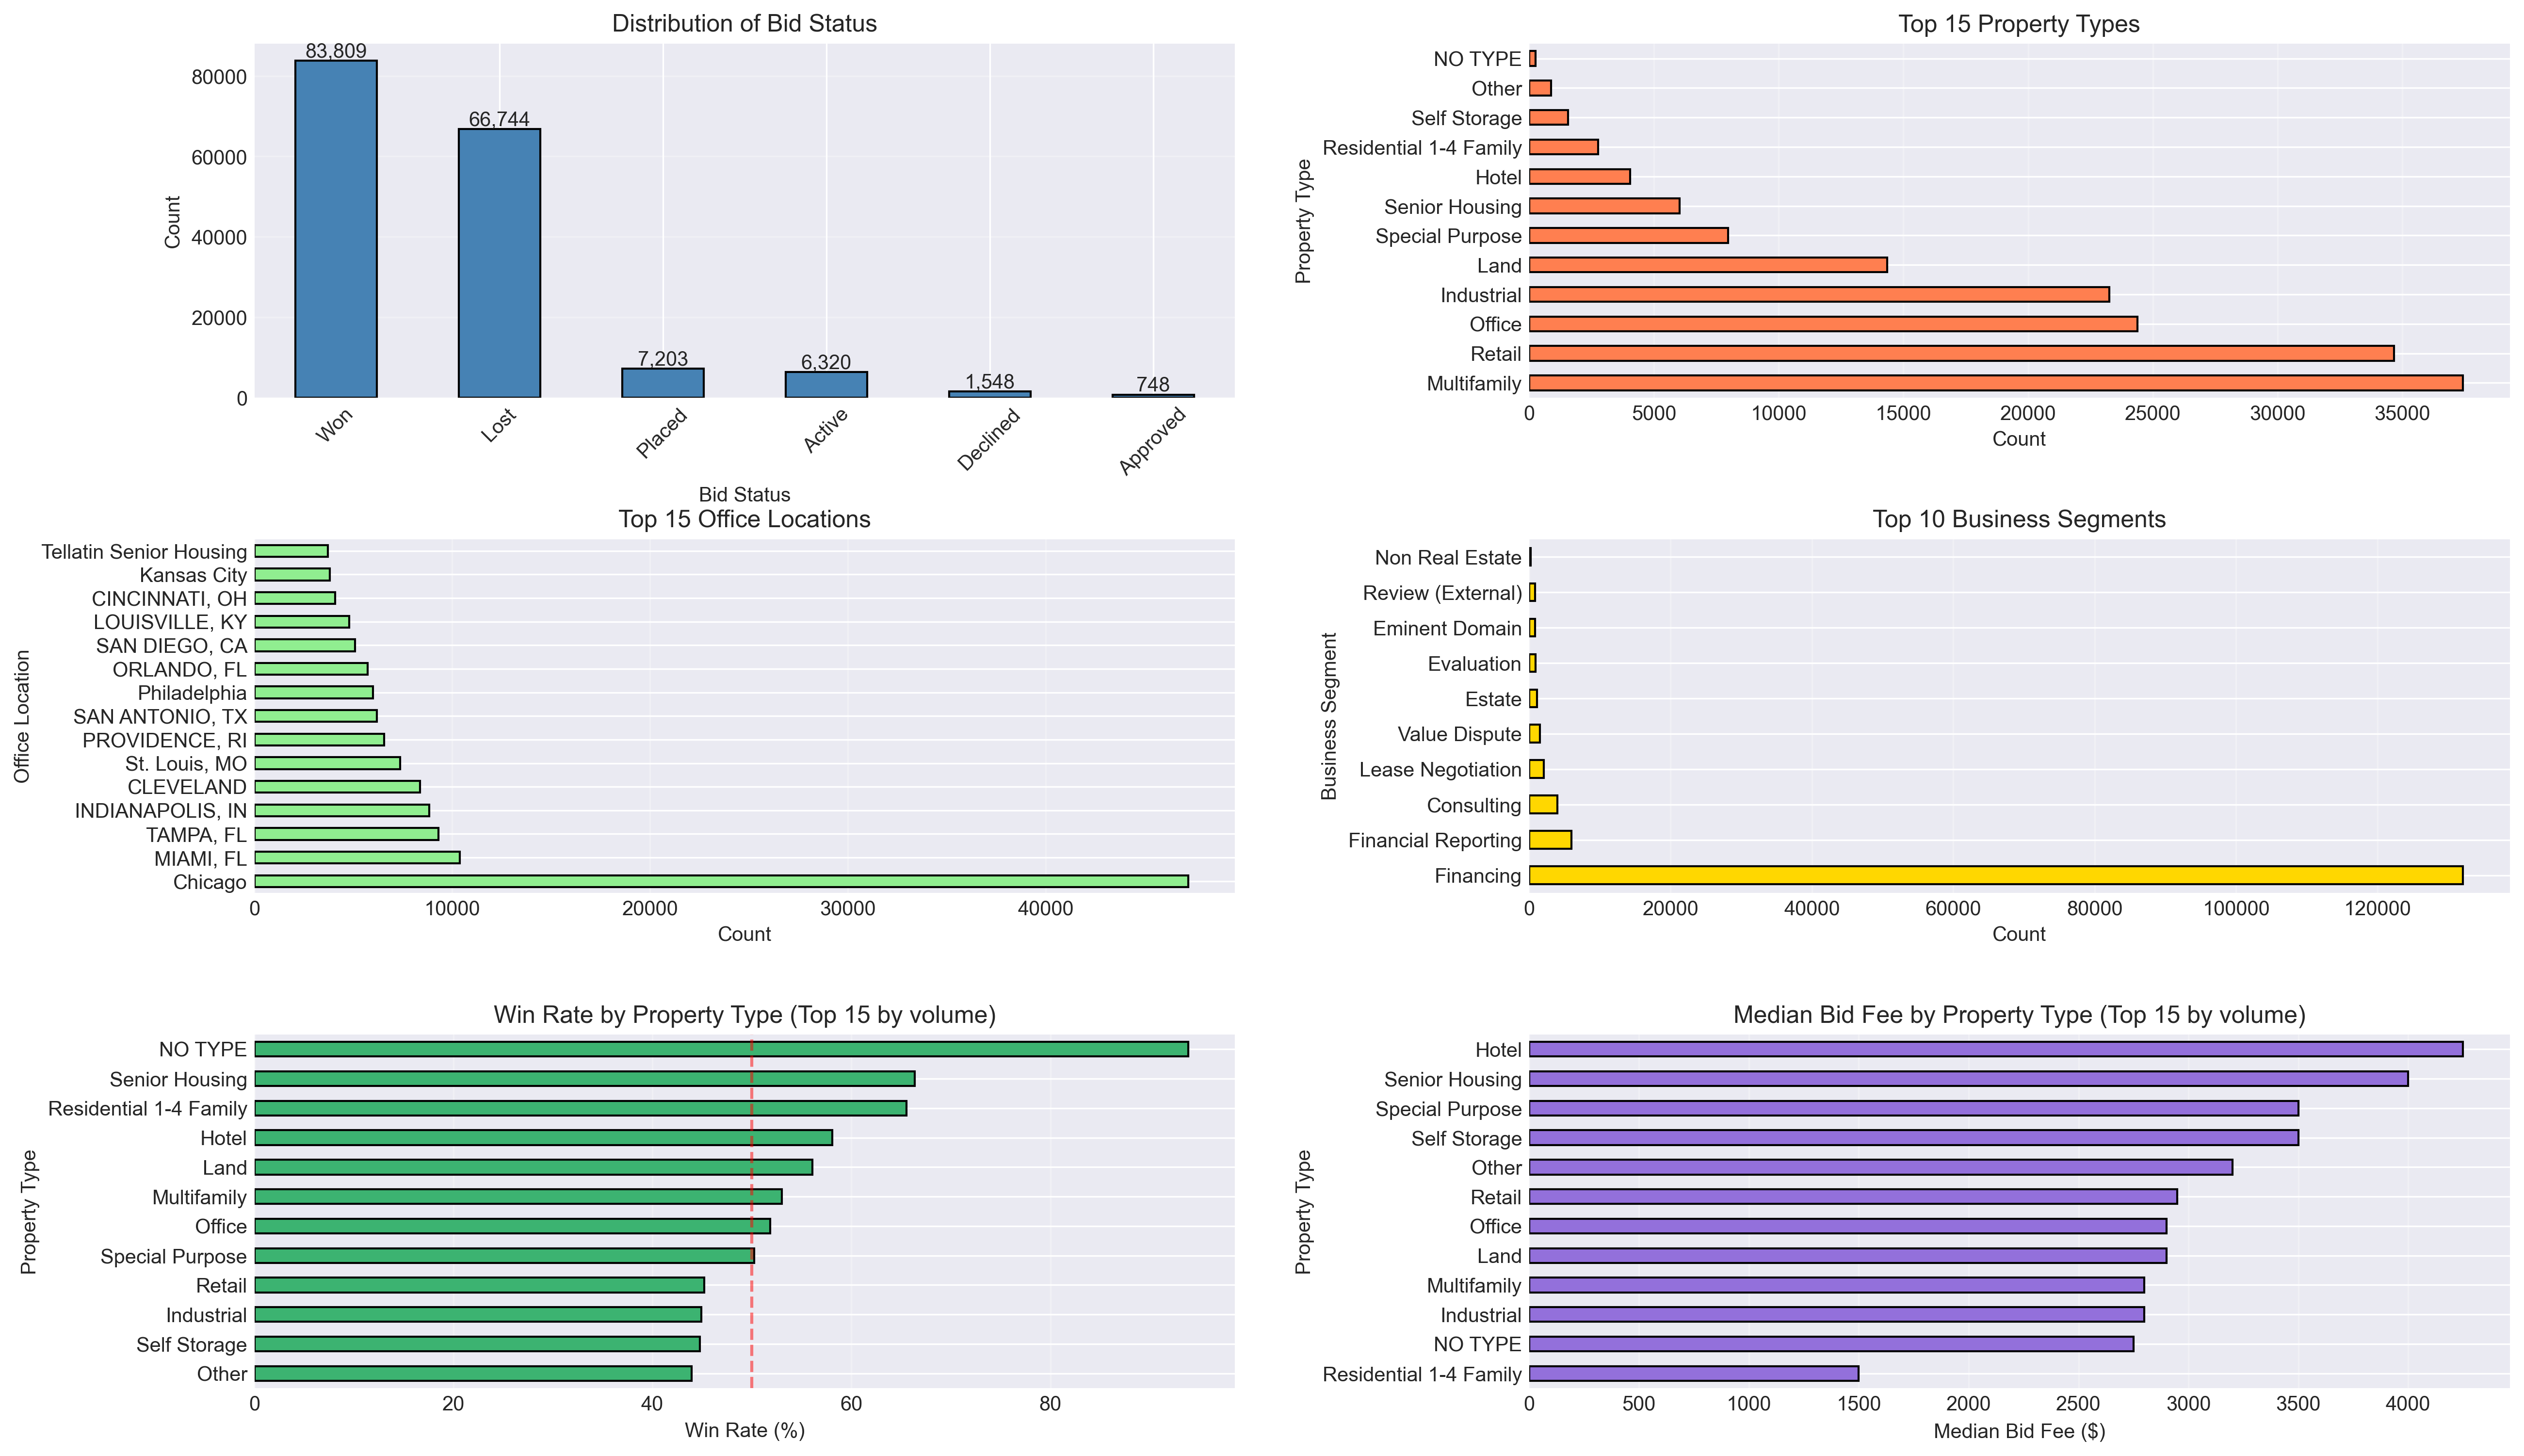
\includegraphics[width=0.85\textwidth]{categorical_features_analysis.png}
\caption{Analysis of categorical features: distribution and relationship with BidFee.}
\label{fig:categorical-analysis}
\end{figure}

\begin{figure}[H]
\centering
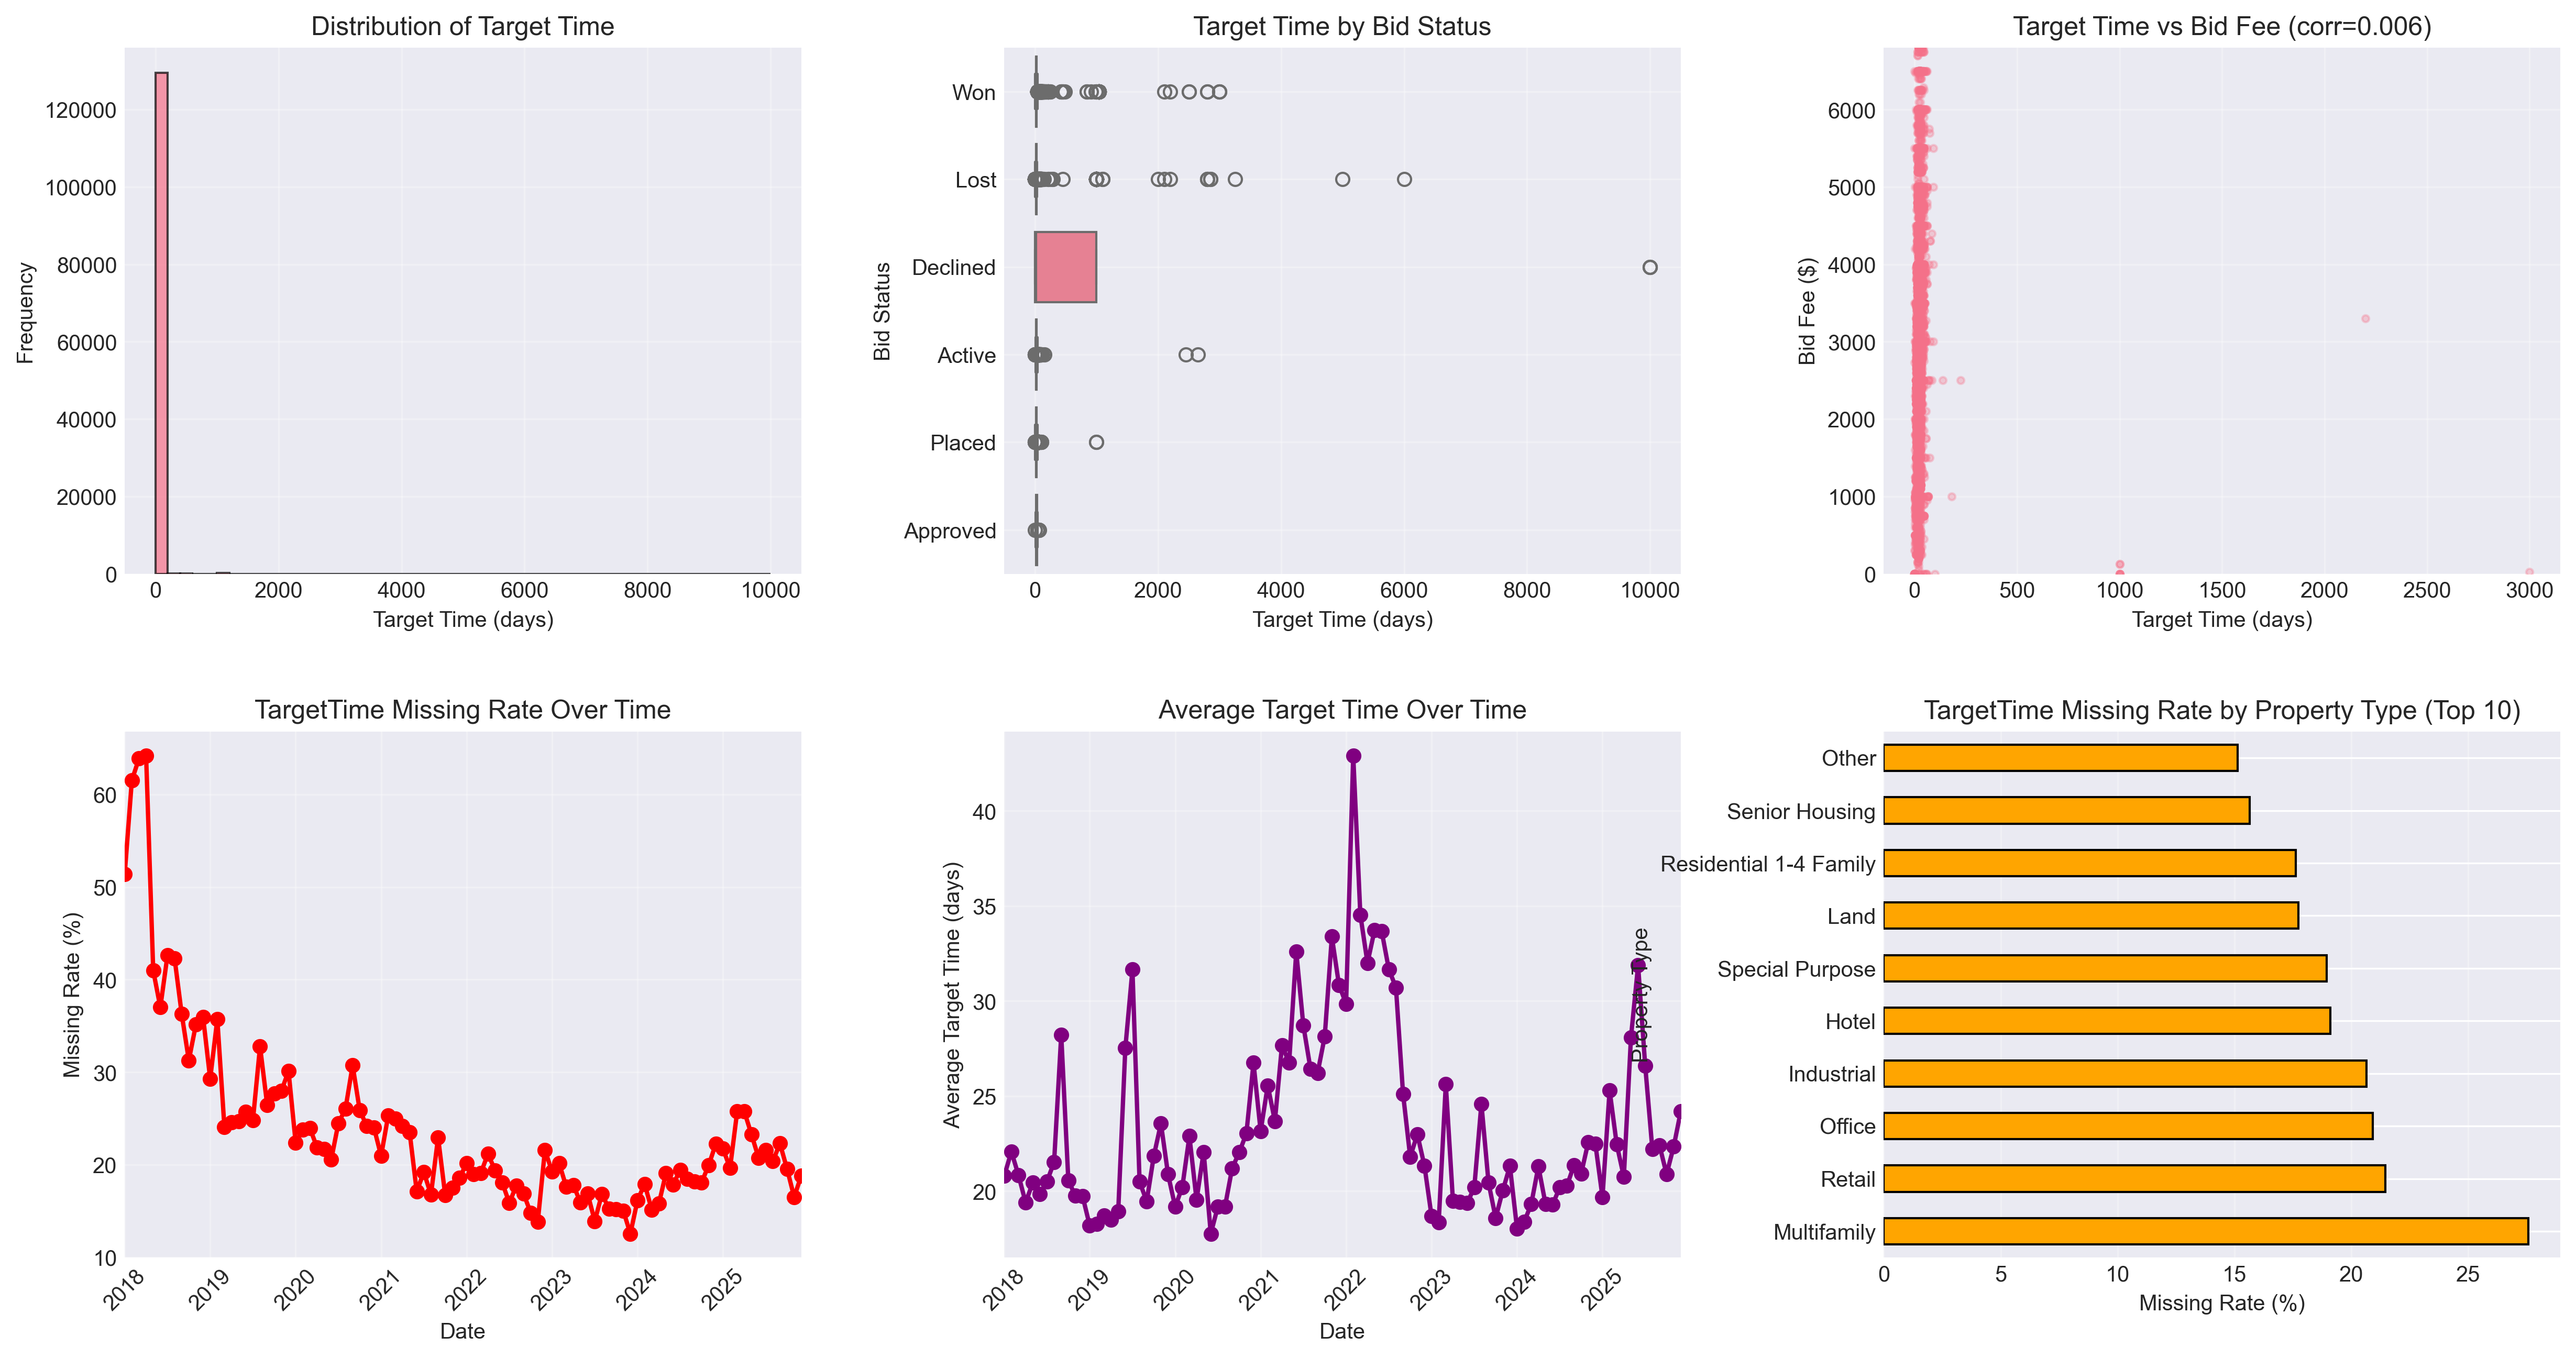
\includegraphics[width=0.85\textwidth]{targettime_analysis.png}
\caption{Target time analysis: distribution and relationship with engagement complexity.}
\label{fig:targettime-analysis}
\end{figure}

\begin{figure}[H]
\centering
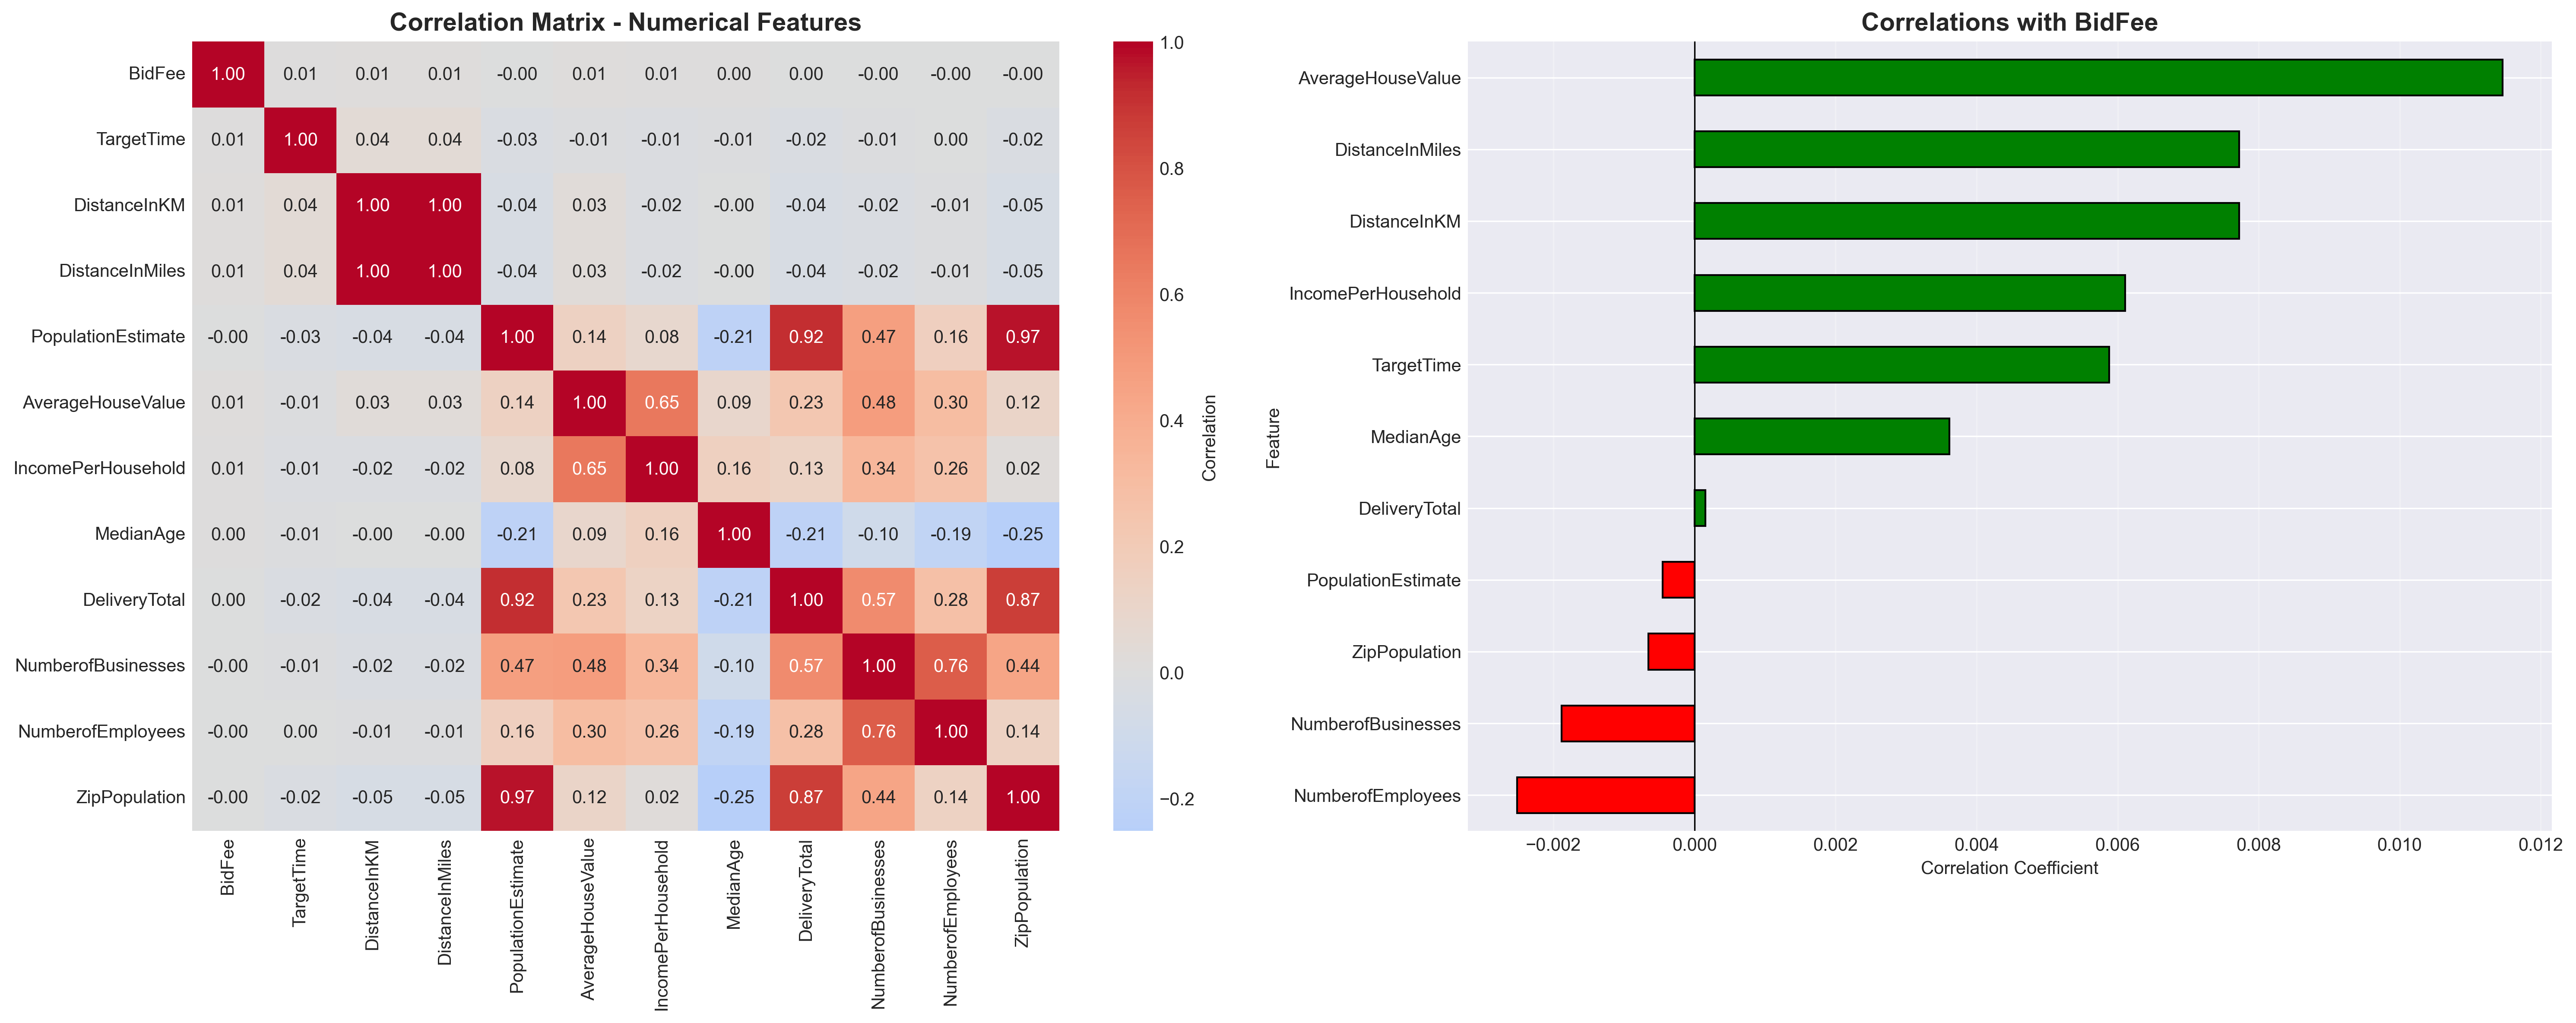
\includegraphics[width=0.85\textwidth]{correlation_analysis.png}
\caption{Feature correlation matrix highlighting weak direct correlations between raw features and BidFee.}
\label{fig:correlation}
\end{figure}

%============================================================================
\section{Supplementary Visualizations}
%============================================================================

\begin{figure}[H]
\centering
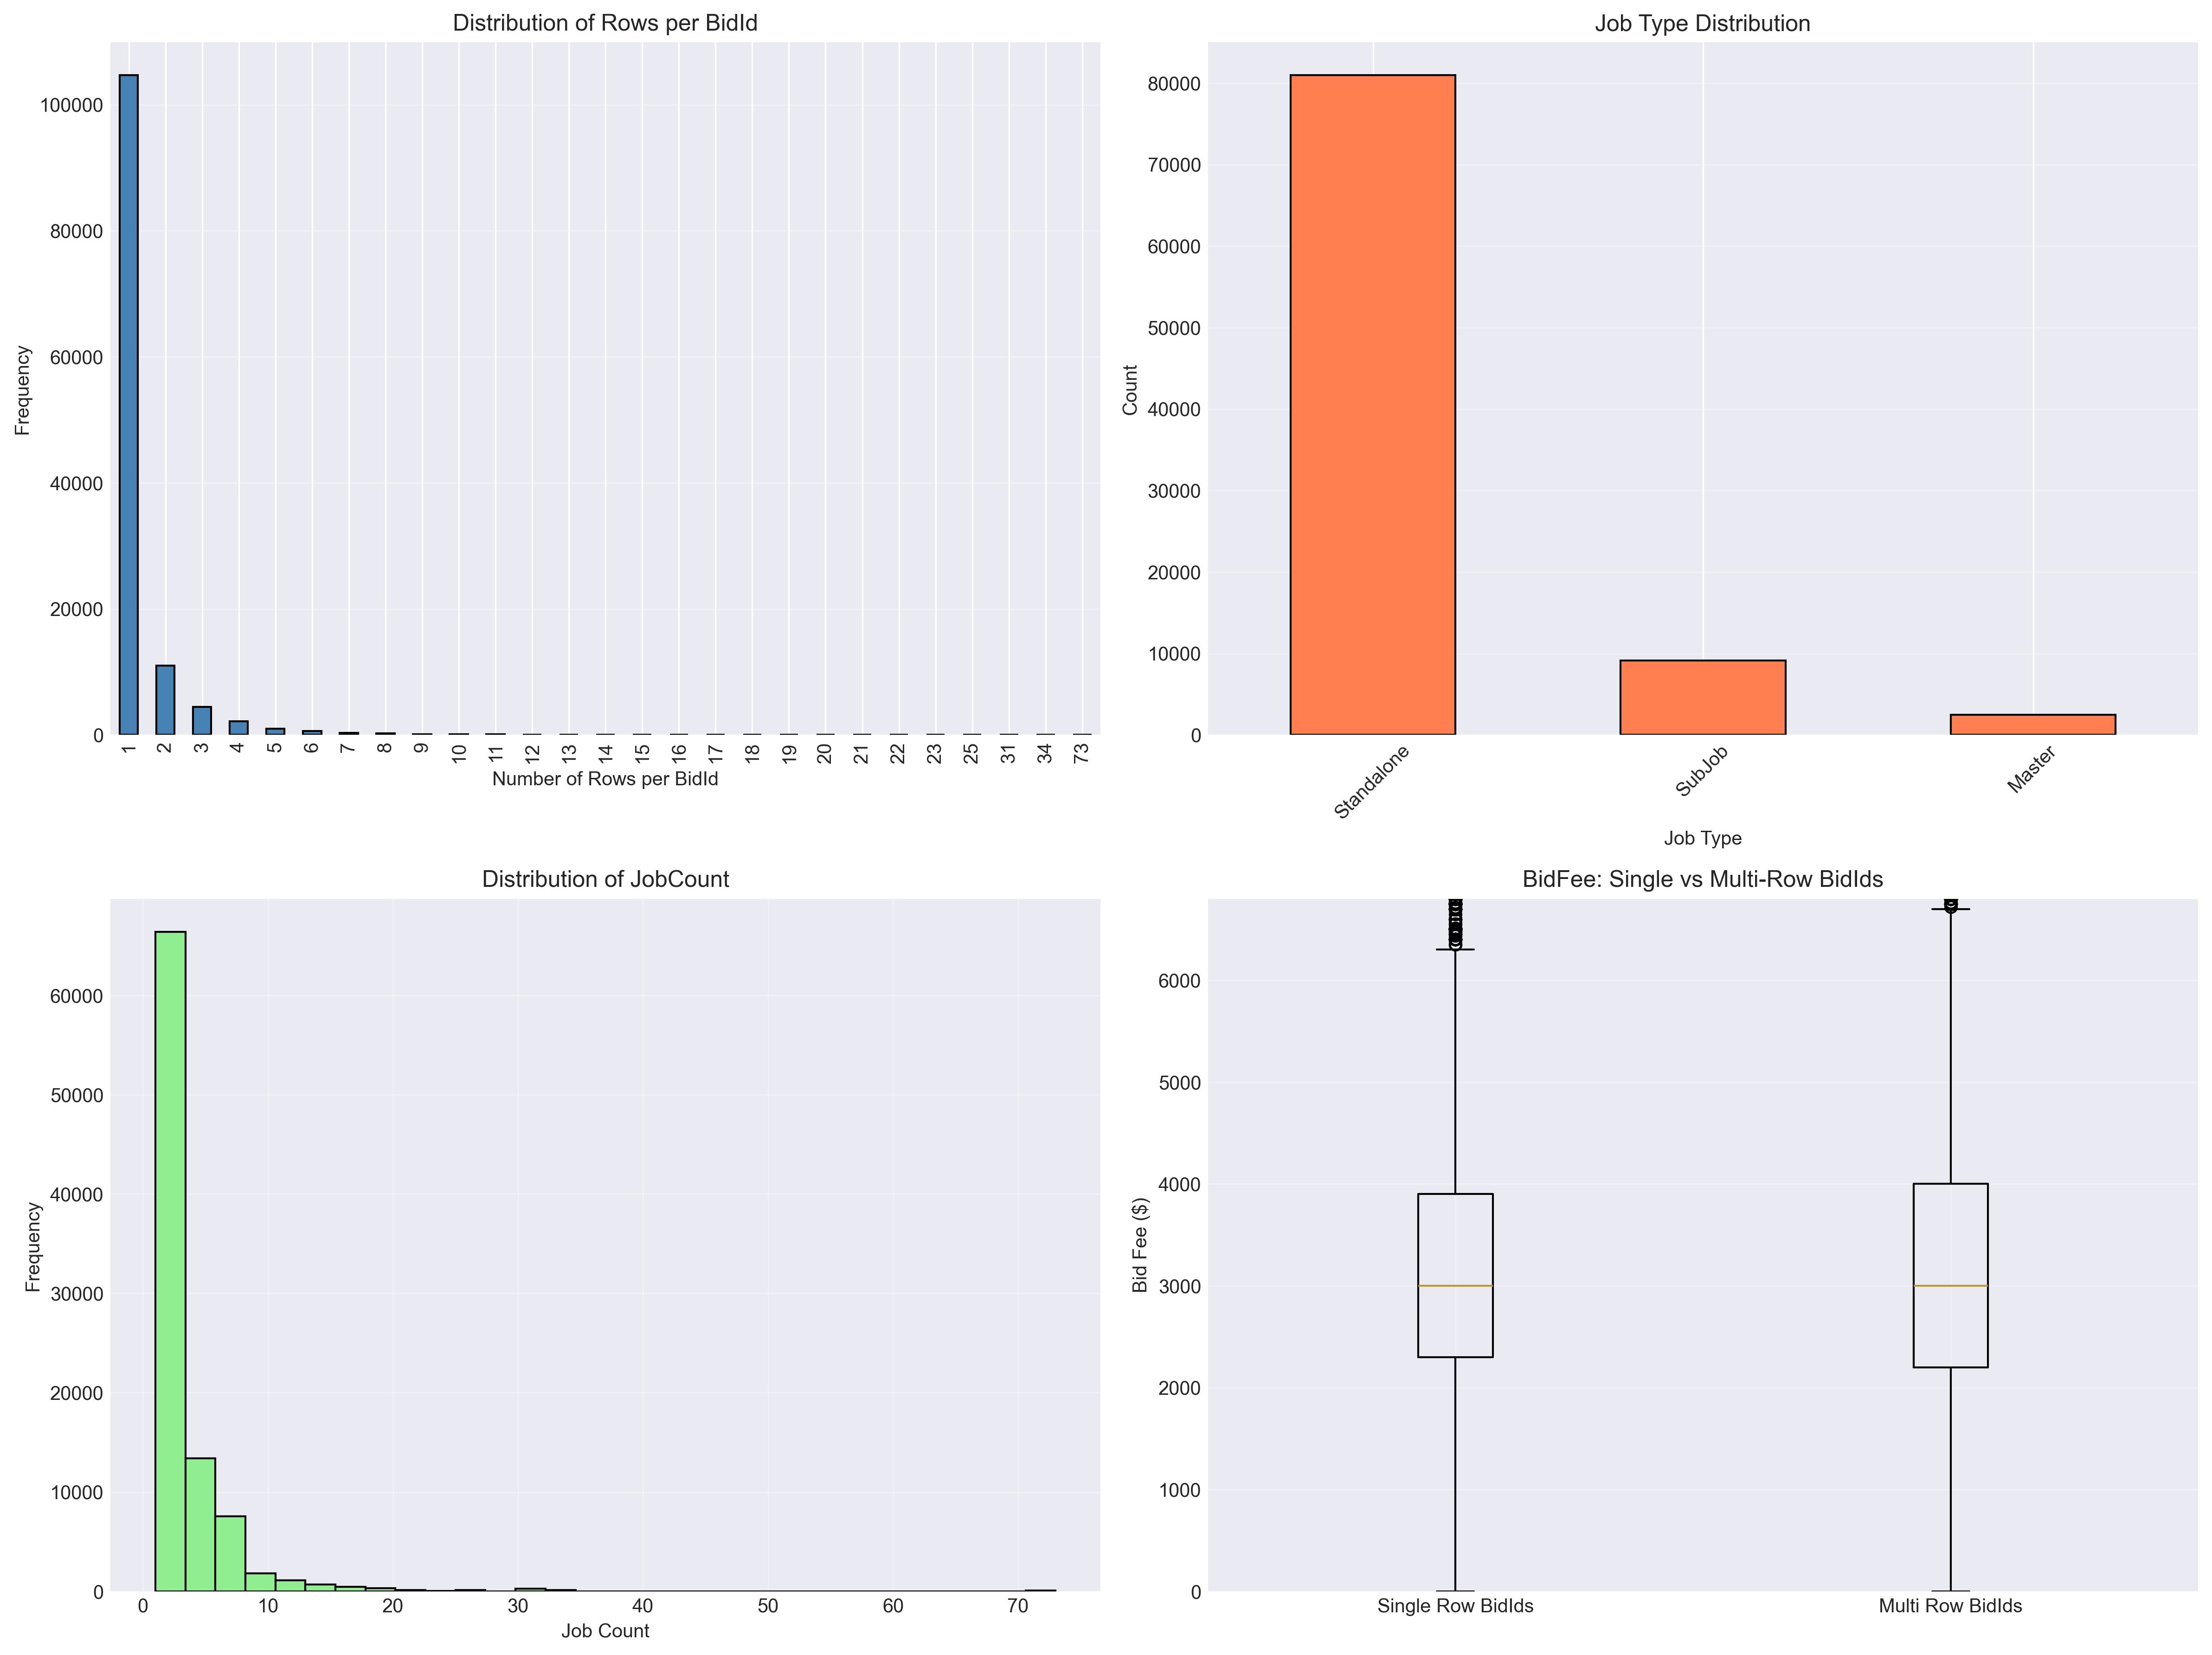
\includegraphics[width=0.85\textwidth]{bid_hierarchy_analysis.png}
\caption{Bid hierarchy analysis: Master/SubJob relationships and their impact on pricing.}
\label{fig:bid-hierarchy}
\end{figure}

\begin{figure}[H]
\centering
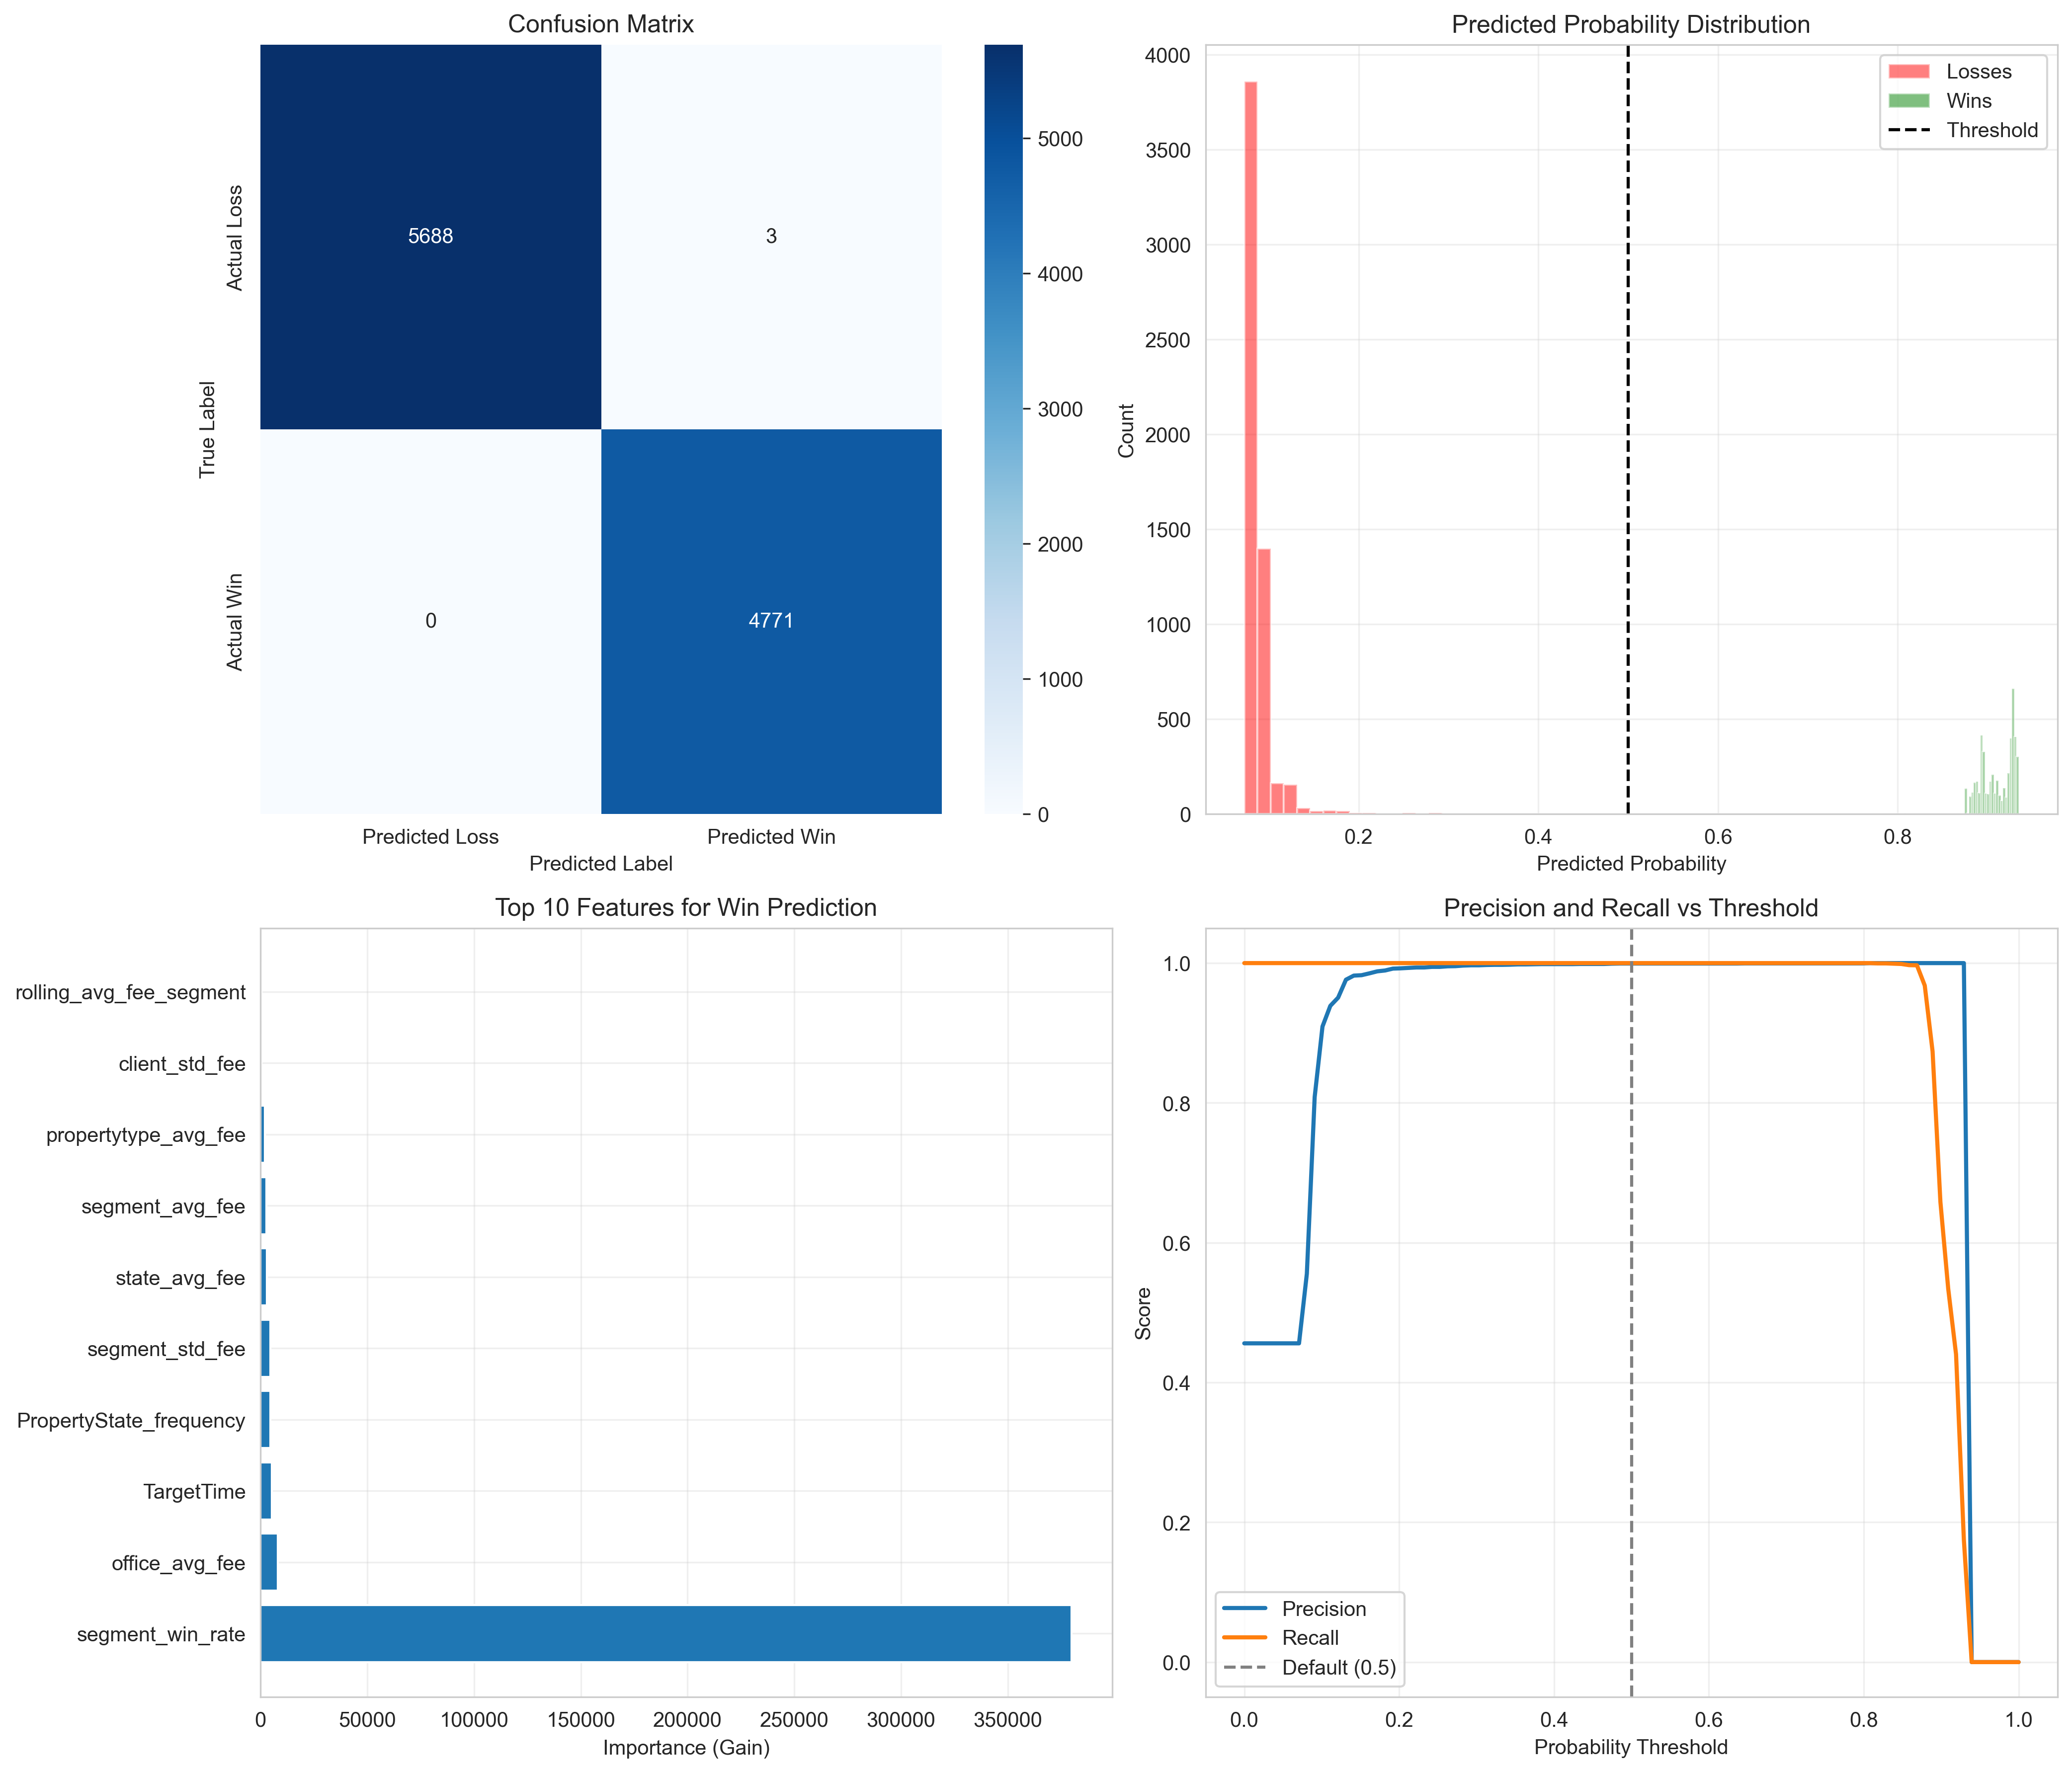
\includegraphics[width=0.85\textwidth]{win_probability_analysis.png}
\caption{Win probability distribution analysis across segments, states, and property types.}
\label{fig:winprob-analysis}
\end{figure}

\begin{figure}[H]
\centering
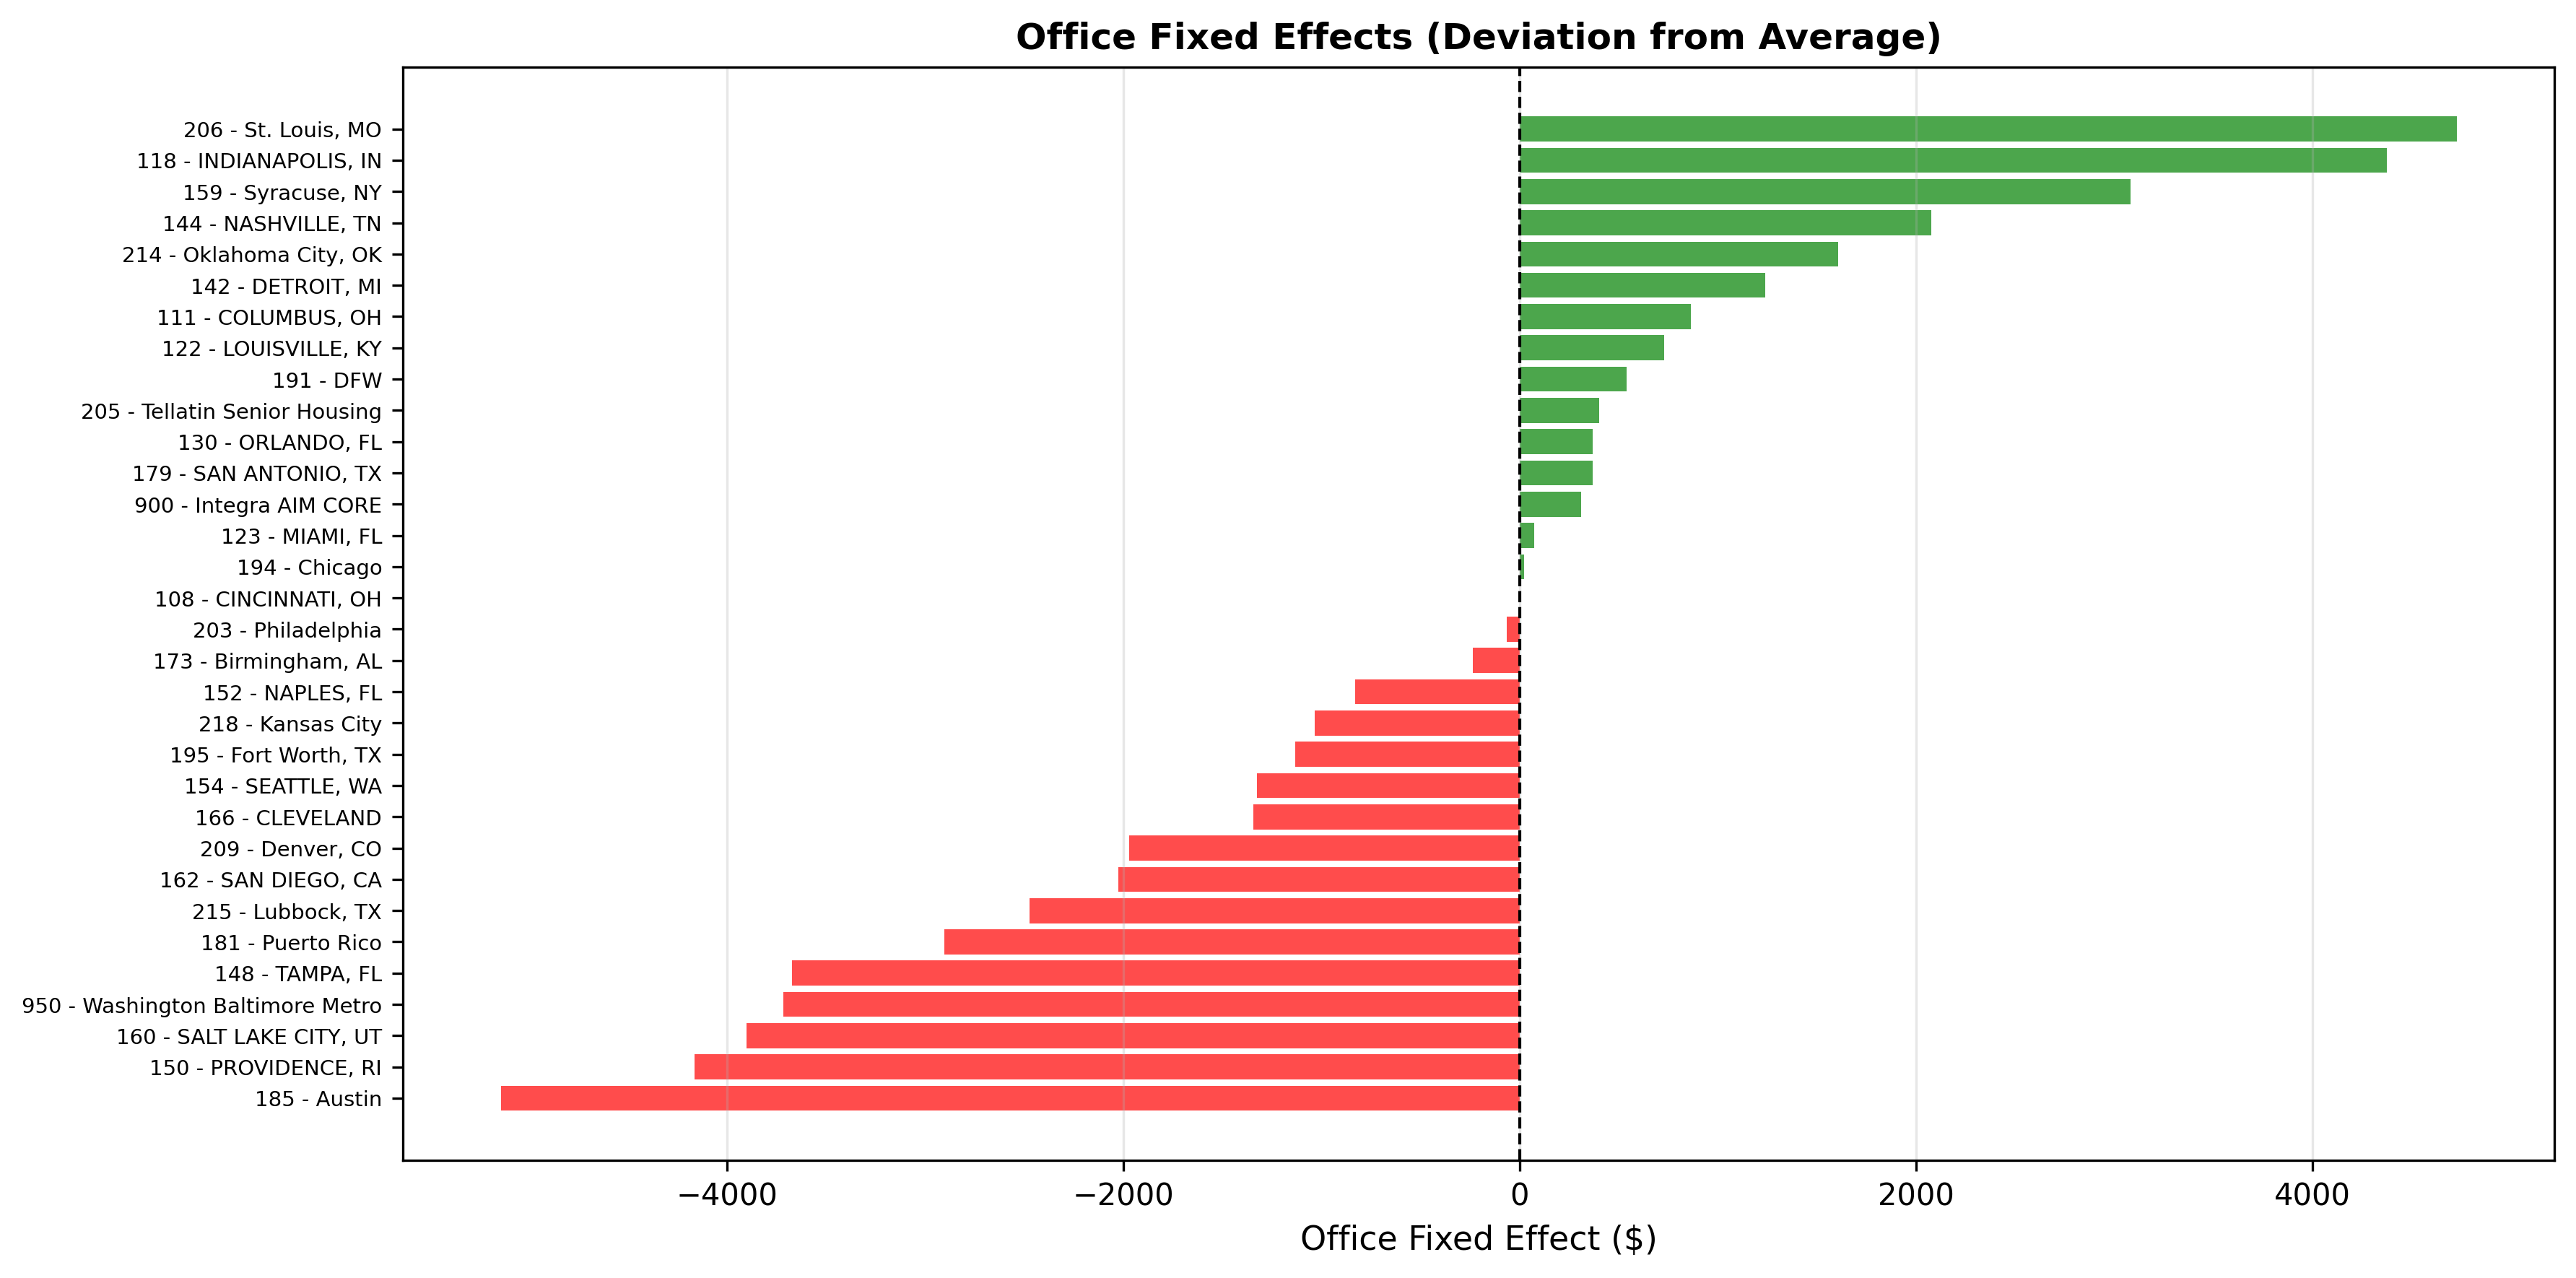
\includegraphics[width=0.85\textwidth]{office_fixed_effects.png}
\caption{Office fixed effects: variation in bid pricing across different office locations.}
\label{fig:office-effects}
\end{figure}

\begin{figure}[H]
\centering
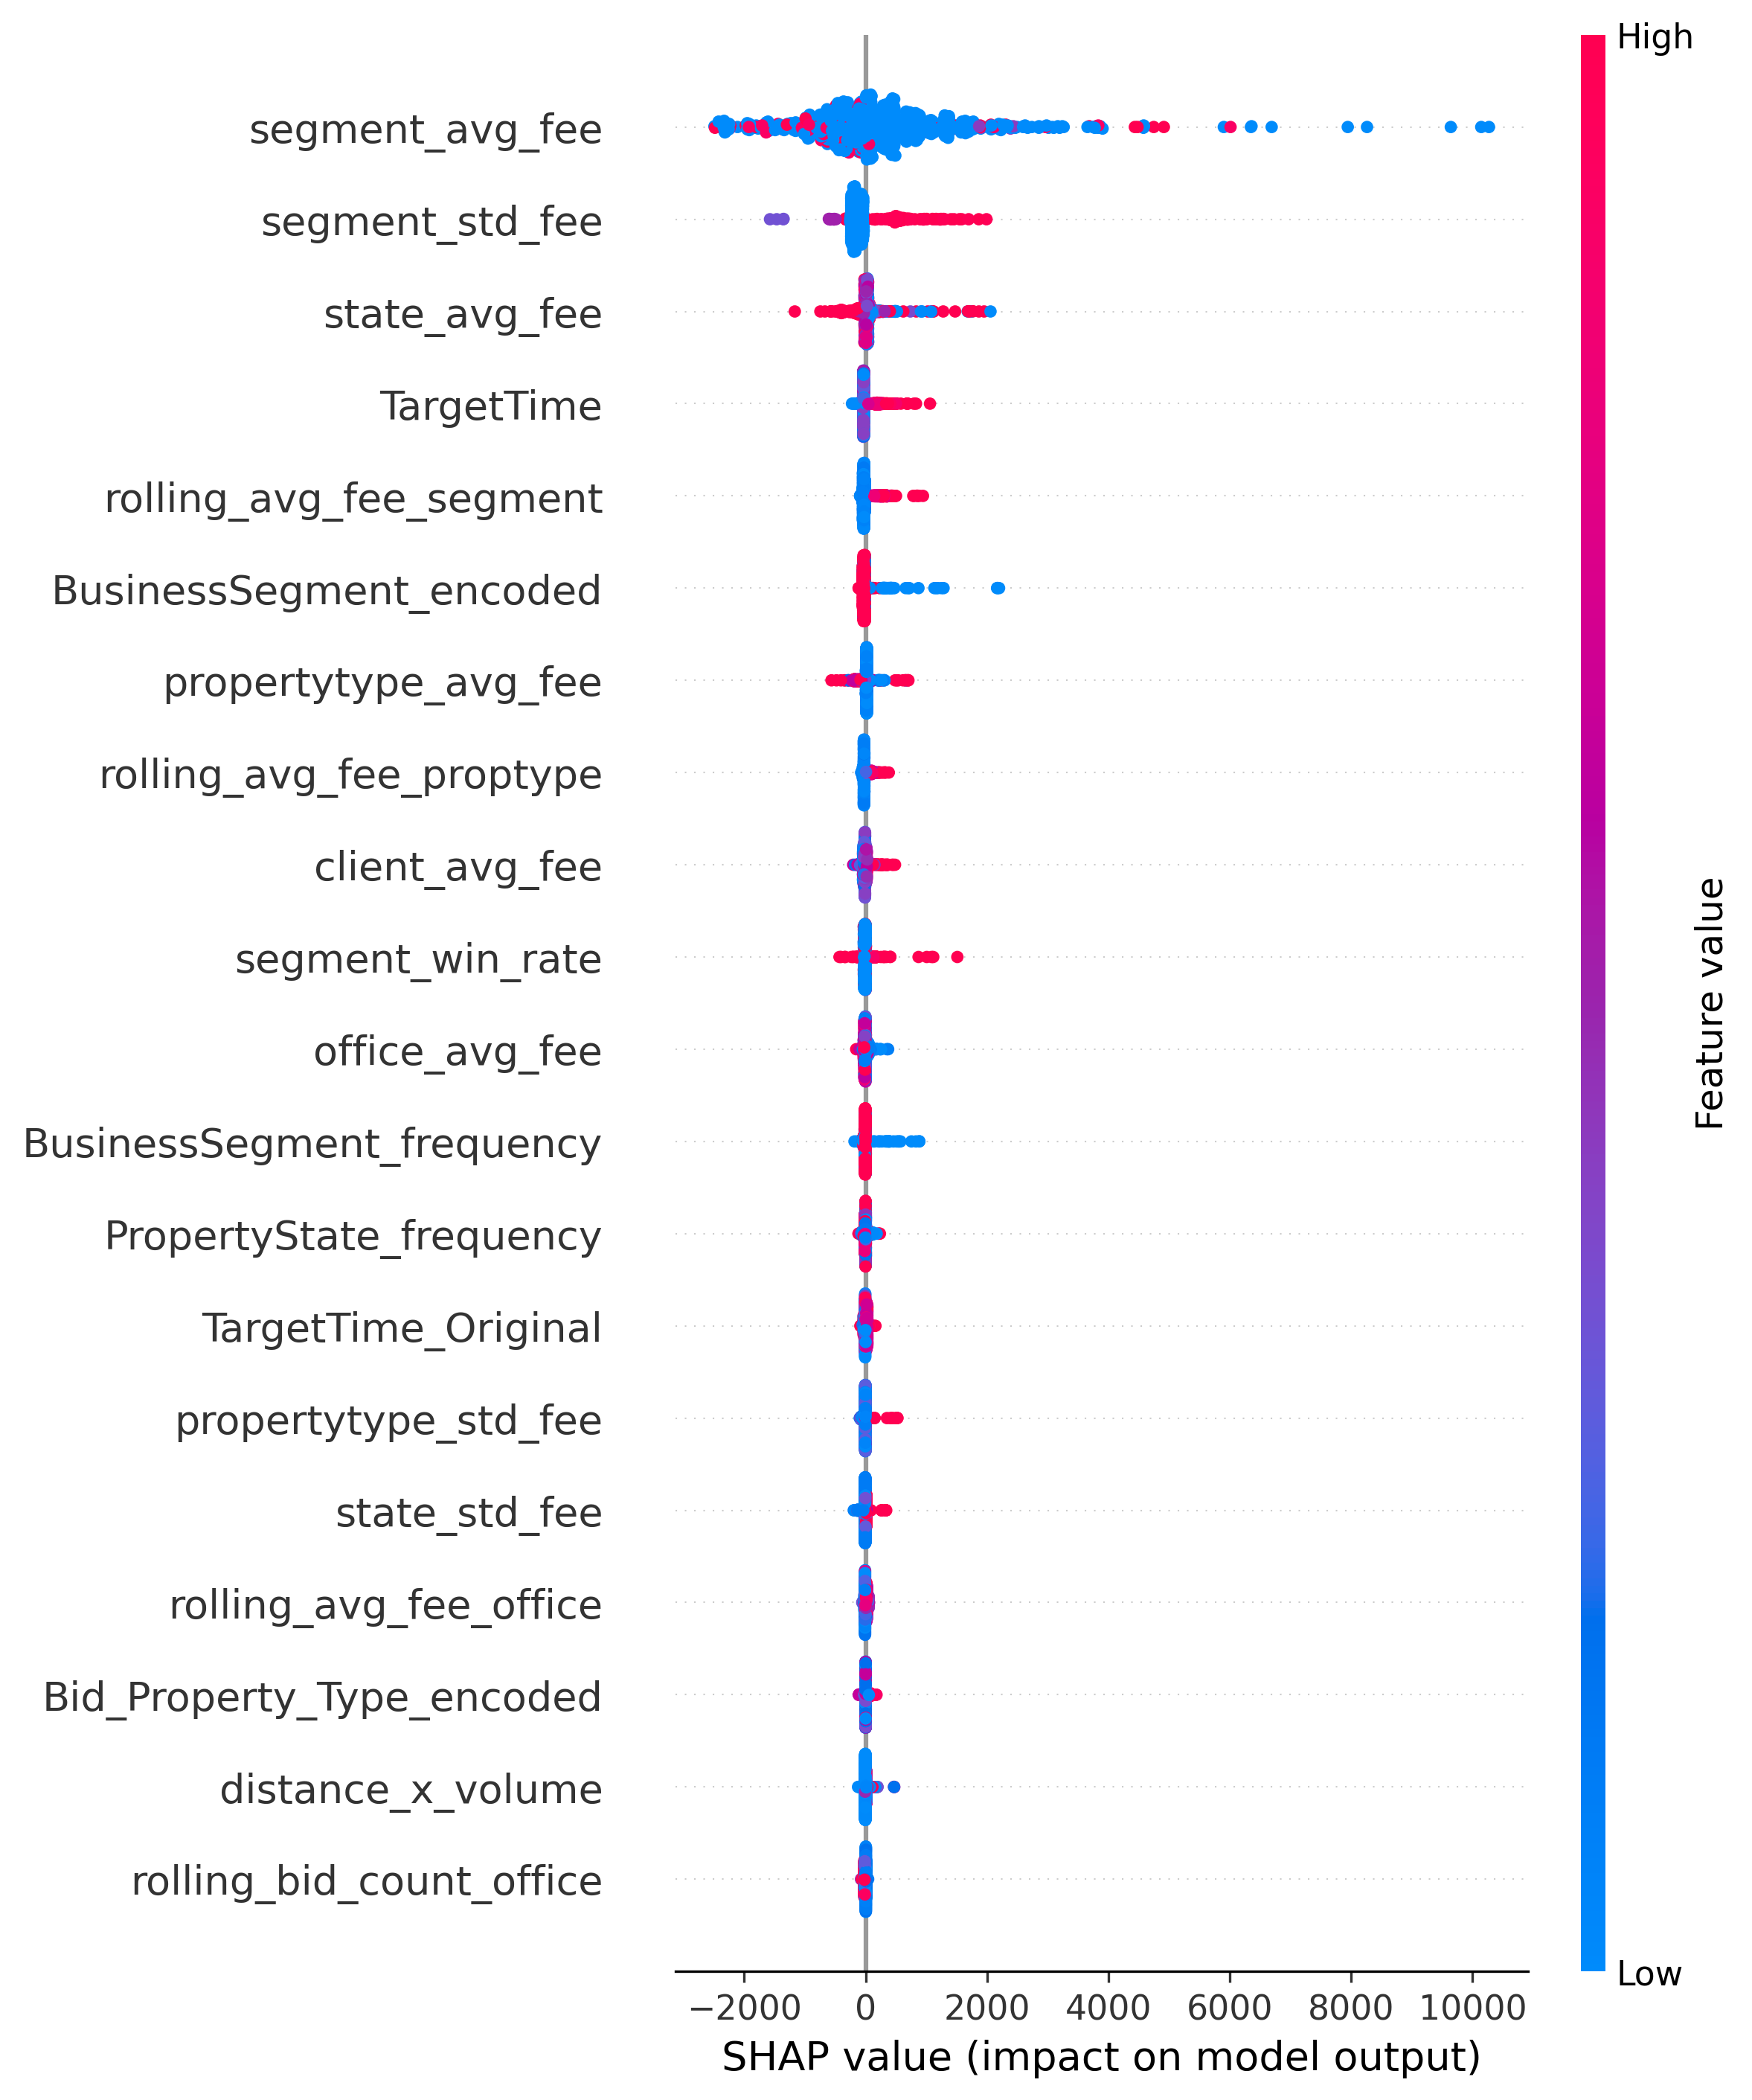
\includegraphics[width=0.85\textwidth]{lightgbm_shap_summary.png}
\caption{SHAP beeswarm plot showing individual feature contributions to bid fee predictions.}
\label{fig:shap-beeswarm}
\end{figure}

%============================================================================
\section{Testing and Validation}
%============================================================================

The system includes a comprehensive test suite with 26 unit tests covering:

\begin{itemize}[nosep]
    \item \textbf{Input validation} (5 tests): Valid input acceptance, missing features detection, out-of-range warnings, negative fee warnings, missing value handling.
    \item \textbf{Confidence logic} (4 tests): State count vs.\ proportion correctness, high-confidence conditions, band-capping behavior, win probability confidence hierarchy.
    \item \textbf{Fee-sensitivity adjustment} (5 tests): Parity behavior, competitive fee boost, aggressive fee penalty, monotonicity, probability clamping (validates the fallback sigmoid formula).
    \item \textbf{Edge cases} (3 tests): Zero segment benchmark, very low fee ratio, exact parity ratio.
    \item \textbf{Response structure} (4 tests): Required keys validation, win probability response keys, valid confidence levels, EV formula correctness.
    \item \textbf{Prediction configuration} (3 tests): Config importability, required keys presence, value reasonableness.
    \item \textbf{Prediction post-processing} (2 tests): Negative clamping, MAPE zero-exclusion.
\end{itemize}

All tests run in CI (GitHub Actions) on Python 3.10 and 3.11 without requiring model files or data.

%============================================================================
\section{Conclusion and Future Work}
%============================================================================

\subsection{Summary of Contributions}

\begin{enumerate}[nosep]
    \item \textbf{Expected Value optimization:} A principled framework for bid pricing that jointly considers fee and win probability.
    \item \textbf{Connected dual-model architecture:} Phase 1A predicts the fee, which feeds directly into Phase 1B as the \texttt{BidFee} feature. The models are architecturally connected, not independent.
    \item \textbf{Data-driven fee-sensitivity:} The win probability model learns fee-win relationships from 52,308 historical outcomes --- no hand-tuned sigmoid parameters.
    \item \textbf{Data integrity:} Identified and removed JobCount leakage (47\% of prior model importance was a cheat code), producing honest, reliable metrics.
    \item \textbf{Unified confidence scoring:} Multi-signal confidence metric with a hierarchy constraint ensuring consistency.
    \item \textbf{Extensive feature engineering:} 68 features for bid fee, 72 for win probability, across 9 categories, with leave-one-out aggregation to prevent leakage.
    \item \textbf{Rigorous benchmarking:} Comparison against econometric panel models and XGBoost, with systematic ablation studies.
    \item \textbf{Production deployment:} Full-stack web application with React frontend and Flask API.
\end{enumerate}

\subsection{Future Work}

\begin{itemize}[nosep]
    \item \textbf{Probability calibration:} Apply Platt scaling or isotonic regression to improve calibration in the 45--75\% probability range where the model is currently slightly overconfident.
    \item \textbf{Log-transform BidFee target:} Training on $\log(\text{BidFee})$ could reduce the high MAPE (71\%) caused by proportionally large errors on small bids.
    \item \textbf{Online learning:} Incremental model updates as new bid outcomes arrive, reducing the staleness of group statistics.
    \item \textbf{Multi-objective optimization:} Optimize for a portfolio of bids simultaneously, considering capacity constraints and revenue targets.
    \item \textbf{Explainability dashboard:} SHAP-based explanations for individual predictions, showing which factors push the fee up or down.
    \item \textbf{A/B testing framework:} Systematic comparison of model recommendations against human pricing decisions.
\end{itemize}

%============================================================================
\appendix
\section{Complete Model Specifications}
%============================================================================

\begin{table}[H]
\centering
\caption{Complete Model Specification Summary}
\label{tab:model-specs}
\begin{tabular}{lll}
\toprule
\textbf{Attribute} & \textbf{Phase 1A (Bid Fee)} & \textbf{Phase 1B (Win Prob)} \\
\midrule
Algorithm & LightGBM GBDT & LightGBM GBDT \\
Objective & Regression (L2) & Binary (log loss) \\
Features & 68 & 72 (incl.\ BidFee) \\
Training samples & 31,384 & 31,384 \\
Validation samples & 10,462 & 10,462 \\
Test samples & 10,462 & 10,462 \\
Best iteration & 500 & 415 \\
Num leaves & 18 & 20 \\
Max depth & 8 & 8 \\
Learning rate & 0.05 & 0.05 \\
Reg alpha & 2.0 & 1.0 \\
Reg lambda & 2.0 & 1.0 \\
Primary metric & RMSE (\$354) & AUC-ROC (0.870) \\
Overfitting ratio & 1.99$\times$ & 1.09$\times$ \\
Model file & \texttt{.txt} format & \texttt{.txt} format \\
Training date & 2026-02-10 & 2026-02-10 \\
\bottomrule
\end{tabular}
\end{table}

\section{Prediction Configuration Parameters}

\begin{table}[H]
\centering
\caption{PREDICTION\_CONFIG Parameters}
\label{tab:pred-config}
\begin{tabular}{llc}
\toprule
\textbf{Parameter} & \textbf{Description} & \textbf{Value} \\
\midrule
\texttt{confidence\_segment\_high} & Min segment count for ``high'' confidence & 1,000 \\
\texttt{confidence\_state\_high} & Min state count for ``high'' confidence & 500 \\
\texttt{confidence\_segment\_medium} & Min segment count for ``medium'' confidence & 100 \\
\texttt{confidence\_state\_medium} & Min state count for ``medium'' confidence & 50 \\
\texttt{band\_ratio\_high} & Max band ratio for ``high'' band confidence & 0.3 \\
\texttt{band\_ratio\_medium} & Max band ratio for ``medium'' band confidence & 0.6 \\
\texttt{win\_prob\_min} & Minimum clamped win probability & 0.05 \\
\texttt{win\_prob\_max} & Maximum clamped win probability & 0.95 \\
\texttt{min\_fee} & Minimum predicted fee floor & \$500 \\
\bottomrule
\end{tabular}
\end{table}

\section{Complete Feature List --- Bid Fee Model (68 Features)}

{\small
\begin{longtable}{clll}
\toprule
\textbf{\#} & \textbf{Feature} & \textbf{Category} & \textbf{Description} \\
\midrule
\endfirsthead
\toprule
\textbf{\#} & \textbf{Feature} & \textbf{Category} & \textbf{Description} \\
\midrule
\endhead
1 & \texttt{segment\_avg\_fee} & Aggregation & Segment mean fee \\
2 & \texttt{state\_avg\_fee} & Aggregation & State mean fee \\
3 & \texttt{propertytype\_avg\_fee} & Aggregation & Property type mean fee \\
4 & \texttt{TargetTime} & Raw & Target turnaround time \\
5 & \texttt{rolling\_avg\_fee\_segment} & Rolling & 90-day segment avg \\
6 & \texttt{rolling\_avg\_fee\_proptype} & Rolling & 90-day property type avg \\
7 & \texttt{segment\_std\_fee} & Aggregation & Segment fee std dev \\
8 & \texttt{client\_avg\_fee} & Aggregation & Client mean fee \\
9 & \texttt{segment\_win\_rate} & Aggregation & Segment win rate \\
10 & \texttt{PropertyState\_frequency} & Encoding & State frequency \\
11 & \texttt{client\_std\_fee} & Aggregation & Client fee std dev \\
12 & \texttt{distance\_x\_volume} & Interaction & Distance $\times$ volume \\
13 & \texttt{state\_std\_fee} & Aggregation & State fee std dev \\
14 & \texttt{TargetTime\_Original} & Raw & Original target time \\
15 & \texttt{office\_avg\_fee} & Aggregation & Office mean fee \\
16 & \texttt{RooftopLongitude} & Raw & Property longitude \\
17 & \texttt{OfficeId} & Raw & Office identifier \\
18 & \texttt{avg\_historical\_fee\_client} & Client & Historical client avg \\
19 & \texttt{rolling\_avg\_fee\_office} & Rolling & 90-day office avg \\
20 & \texttt{propertytype\_std\_fee} & Aggregation & Prop type std dev \\
21--68 & \multicolumn{3}{l}{\textit{Remaining features include office/client/temporal/encoding/interaction features}} \\
\bottomrule
\end{longtable}
}

%============================================================================
\end{document}
